% High-dimensional Gaussian approximation over rectangles.
% Manuscript revised 4 November 2026.
\documentclass[11pt,letterpaper]{article}
\usepackage[margin=1.05in]{geometry}
\usepackage[T1]{fontenc}
\usepackage{lmodern,microtype}
\usepackage{amsmath,amssymb,amsthm,mathtools}
\usepackage{longtable,booktabs,tabularx}
\usepackage{tikz}
\usetikzlibrary{arrows.meta}
\usepackage[hidelinks,hypertexnames=false,linktoc=all]{hyperref}
\newcommand{\Ac}{\mathsf A}
\usepackage{fancyhdr}
\pagestyle{fancy}
\fancyhf{}
\fancyhead[L]{\small Gaussian approximation over rectangles}
\fancyhead[R]{\small\thepage}
\setlength{\headheight}{14pt}
\hypersetup{pdftitle={High-Dimensional Gaussian Approximations over Rectangles without Covariance Restrictions},pdfsubject={Independent sums with bounded, sub-exponential, or polynomial-moment envelopes},pdfauthor={Victor Chernozhukov, Denis Chetverikov, Kengo Kato, Yuta Koike}}
\setlength{\parindent}{1.25em}
\setlength{\parskip}{0pt}
\emergencystretch=2em
\allowdisplaybreaks[2]
\raggedbottom
\clubpenalty=10000
\widowpenalty=10000
\newtheorem{theorem}{Theorem}
\newtheorem{proposition}{Proposition}
\newtheorem{lemma}{Lemma}
\newtheorem{corollary}{Corollary}
\newtheorem{conjecture}{Conjecture}
\theoremstyle{remark}
\newtheorem{remark}{Remark}
\newcommand{\E}{\mathbb E}
\newcommand{\Pp}{\mathbb P}
\newcommand{\R}{\mathbb R}
\newcommand{\cR}{\mathcal R}
\newcommand{\cF}{\mathcal F}
\newcommand{\cP}{\mathcal P}
\newcommand{\cD}{\mathcal D}
\newcommand{\Cov}{\operatorname{Cov}}
\newcommand{\Var}{\operatorname{Var}}
\newcommand{\tr}{\operatorname{tr}}
\newcommand{\op}{\mathrm{op}}
\newcommand{\norm}[1]{\left\lVert#1\right\rVert}
\newcommand{\maxnorm}[1]{\lVert#1\rVert_{\max}}
\newcommand{\rh}{\rho_{\mathcal R}}
\newcommand{\ind}{\mathbf 1}
\newcommand{\dd}{\,d}
\newcommand{\Hh}{H_2}
\newcommand{\surf}{\mathcal J}

\newcommand{\logp}{\log_+}

\begin{document}
\begin{center}
{\Large High-Dimensional Gaussian Approximations\\[0.15em]
over Rectangles without Covariance Restrictions}\\[0.85em]
{\normalsize Victor Chernozhukov, Denis Chetverikov, Kengo Kato, Yuta
Koike\renewcommand{\thefootnote}{\fnsymbol{footnote}}\footnote{The paper
was developed through collaboration with the AI systems GPT-6 Astra,
GPT-6 Sol, and Claude Opus.}}\\[0.65em]
{\normalsize 4 November 2026 \(\,\cdot\,\) Unrestricted covariance, split-V2}
\end{center}
\setcounter{footnote}{0}
\thispagestyle{plain}

\begin{abstract}

We study Gaussian approximation over rectangles for a sum of independent
centered random vectors. We require positive marginal variances and allow
arbitrary dependence among the coordinates, including exact linear dependence.
For \(n\) observations bounded coordinatewise by \(B\), with unit marginal
variances after normalization, the approximation error is at most
\[
 C\,\frac{B L^{3/2}}{\sqrt n}
 \sqrt{1+\log_+\!\left(\frac{\sqrt n}{B\sqrt L}\right)},
 \qquad L:=\log(ep),\quad \log_+x:=\max\{0,\log x\}.
\]
A refinement charges a fourth-moment bound relative to the covariance for the logarithmic term. It removes the extra logarithmic factor when large summands contribute little to the variance in every standardized direction. A bounded symmetric example attains the \(n^{-1/2}L^{3/2}\) scale for a fixed
envelope. Whether the remaining logarithm can be removed is open.
Clipping gives a corresponding result for sub-exponential coordinates.
For polynomial moment envelopes the rate changes with the moment order.
At order \(4\), under a separate coordinate fourth-moment bound, symmetric
examples attain the \(n^{-1/4}L^{5/4}\) rate for a fixed envelope.
For growing envelopes, the upper and lower bounds also match in their
dependence on \(B\) in the dimension regimes specified below.
\end{abstract}

\begingroup
\setcounter{tocdepth}{1}
\small
\tableofcontents
\endgroup
\clearpage

\section{\texorpdfstring{Introduction and main results}{Introduction and main results}}\label{sec:results}
Gaussian approximation over rectangles provides a common foundation for
approximating maxima and constructing simultaneous confidence regions, with
applications to a wide variety of statistical inference problems reviewed in~\cite{CCKK2023}.
In many of these applications the correlation matrix may be nearly or
exactly singular. We obtain approximation bounds that remain uniform
as its eigenvalues approach zero. For example, if two measured outcomes
coincide, their correlation is \(1\), yet both coordinates are covered
by the same theorem. How accurately we can approximate the sum depends on how large a
single observation can be.

Table~\ref{opt:tab:rates} in Section~\ref{opt:section} summarizes the upper
and lower bounds we prove in this paper for \(n\) observations in \(p\)
dimensions. In every regime listed, the two bounds differ by at most a
logarithmic factor. For bounded observations, both have sample-size
power \(n^{-1/2}\), even under central symmetry. Under fourth-moment
bounds on the maximum absolute coordinate and on each individual
coordinate, the rate for a fixed envelope is
\(n^{-1/4}(\log p)^{5/4}\). Symmetric examples attain this rate and, in
the growing-envelope regime, also attain the upper bound's dependence on
the envelope size. For other moment orders \(q>2\), the bounds match in
the sparse regime specified in the table. For \(q>4\) and a fixed envelope,
they differ by at most a factor of \(\{\log(en)\}^{1/2-1/q}\).

Let \(W\) be a sum of independent centered bounded random vectors in
\(\R^p\). Suppose that each coordinate of the sum has unit variance,
and let \(Z\) be a centered Gaussian vector with the same covariance.
For the bounded-observation results, our assumptions and notation are
\begin{equation}
 \begin{gathered}
 W\coloneqq (W_j)_{j=1}^p=\sum_{i=1}^n\xi_i,\qquad
 \E\xi_i=0,\qquad \norm{\xi_i}_\infty\le\delta\quad\text{a.s.},\\
 \Sigma\coloneqq \Cov(W),\qquad\Sigma_{jj}=1\ (j\le p),
 \qquad Z\sim N(0,\Sigma),
 \end{gathered}
 \label{eq:setup}
\end{equation}
where $\|\cdot\|_\infty$ denotes the maximum norm of a vector. 
The summands need not have the same distribution, and coordinates within
a summand may be dependent. The unit marginal variances fix the scale
of each coordinate, and they can be obtained by coordinatewise rescaling
whenever all marginal variances are positive. There is no
restriction on the rank of \(\Sigma\).

The parameter \(\delta\) bounds the contribution of any one summand
to any coordinate of \(W\), and such a uniform bound is called an
\emph{envelope}. To state the
bound compactly, put
\[
 L\coloneqq \log(ep),\qquad
 D_L\coloneqq 1+\log_+\frac1{\delta\sqrt L},\qquad
 \log_+x\coloneqq \max\{0,\log x\}.
\]
Here \(L\) encodes the dependence on dimension, while \(D_L\)
contributes an additional logarithmic factor. Constants denoted by
\(C\) are absolute unless a subscript records their dependence.

Let \(\mathcal R\) denote the class of axis-aligned rectangles in
\(\R^p\). We measure the approximation error by the \emph{Kolmogorov distance over rectangles}
\[
 \rh(W,Z)\coloneqq \sup_{A\in\mathcal R}
       |\Pp(W\in A)-\Pp(Z\in A)|.
\]
We use the same notation for any two random vectors in \(\R^p\). For
example, taking \(A\coloneqq (-\infty,s]^p\) shows that this distance controls the
error in approximating the distribution of \(\max_{j\le p}W_j\), the maximum
coordinate of \(W\).

The envelope is needed to smooth the boundary of a rectangle. We can measure the fourth-order comparison error more closely by keeping the moments in each direction where the proof integrates by parts. For $1\le j\le p$, define
\begin{align*}
 T_j&:=\sum_i\E[\xi_{ij}\,\xi_i\xi_i^\top],&
 Q_j&:=\sum_i\E[\xi_{ij}^2\,\xi_i\xi_i^\top],&
 \widetilde Q_j&:=\sum_i\E[\xi_{ij}^2]\,\E[\xi_i\xi_i^\top].
\end{align*}
We call $s_3,s_4\ge0$ \emph{relative moment bounds} if
\begin{equation}\label{eq:relative-moments}
 -s_3\Sigma\preceq T_j\preceq s_3\Sigma,\qquad
 Q_j\preceq s_4\Sigma,\qquad \widetilde Q_j\preceq s_4\Sigma
 \qquad (1\le j\le p).
\end{equation}
For a contrast $u$ of variance $u^\top\Sigma u=1$, the first inequality bounds the absolute signed sum $\sum_i\E[\xi_{ij}(u^\top\xi_i)^2]$. The next two inequalities bound the fourth moments when the coordinate and the contrast come from the same row or from independent copies of it. These comparisons require no inverse of $\Sigma$. The envelope always permits $s_3=\delta$ and $s_4=\delta^2$, by testing on any $u$ and using $|\xi_{ij}|\le\delta$.

\begin{theorem}[Unrestricted covariance]\label{thm:unrestricted}
Under~\eqref{eq:setup}, for every admissible $s_4$ in \eqref{eq:relative-moments},
\begin{equation}\label{eq:relative-unrestricted}
 \rh(W,Z)\le C\min\{1,\,L^{3/2}(\delta+\sqrt{s_4D_L})\}.
\end{equation}
In particular, the envelope alone gives
\begin{equation}
 \rh(W,Z)\le C\min\{1,\delta L^{3/2}\sqrt{D_L}\}.
 \label{eq:unrestricted}
\end{equation}
\end{theorem}
The rate in \eqref{eq:relative-unrestricted} is $O(\delta L^{3/2})$ whenever $s_4D_L\lesssim\delta^2$. Aggregate third moments enter the proof through $s_3L^{3/2}$. Even at exact cancellation, smoothing still costs order $\delta L^{3/2}$ in this argument. A smaller $s_3$ alone therefore yields no gain in the order of the unrestricted bound.

For example, let $\xi_i=a_i R_i$ for independent copies of a centered sign vector with covariance $\Sigma$, where $\sum_i a_i^2=1$. Since $R_{ij}^2=1$, both fourth-moment matrices equal $(\sum_i a_i^4)\Sigma$. Give one row weight proportional to $\sqrt{\log n}$ and the other $n-1$ rows weight proportional to one. After normalization, $\delta\asymp\sqrt{(\log n)/n}$ and $s_4\asymp1/n$. For $p\asymp n^a$ with fixed $a>0$, \eqref{eq:relative-unrestricted} gains a factor of order $\sqrt{\log n}$ over \eqref{eq:unrestricted}, for every covariance of the sign vector.

For normalized observations, Theorem~\ref{thm:unrestricted} gives
the following dependence on the sample size.

\begin{corollary}[Normalized observations]\label{cor:observations}
Let \(X_1,\ldots,X_n\in\R^p\) be independent and centered. Suppose
\(\norm{X_i}_\infty\le B\) almost surely and
\(n^{-1}\sum_i\E X_{ij}^2=1\) for every \(j\). Then, with
\(W_n\coloneqq n^{-1/2}\sum_iX_i\) and \(Z_n\sim N(0,\Cov(W_n))\),
\begin{equation}
 \rh(W_n,Z_n)\le C\min\!\left\{1,
 \frac{B L^{3/2}}{\sqrt n}
 \sqrt{1+\log_+\frac{\sqrt n}{B\sqrt L}}\right\}.
 \label{eq:observations-unrestricted}
\end{equation}
\end{corollary}

Corollary~\ref{cor:observations} follows from Theorem~\ref{thm:unrestricted}
by setting \(\xi_i\coloneqq X_i/\sqrt n\), which has envelope \(\delta=B/\sqrt n\). For
fixed \(B\) and \(p\asymp n^a\), with fixed \(a>0\), its bound has
order \(n^{-1/2}(\log n)^2\).

The factor \(BL^{3/2}/\sqrt n\) is sharp. For \(B\ge2\), \(p\to\infty\) and
\(BL^{3/2}/\sqrt n\to0\), Theorem~\ref{opt:skew-lower} gives i.i.d.\ observations
with independent coordinates whose error is at least of order
\(BL^{3/2}/\sqrt n\). The example is inspired by that of Chernozhukov,
Chetverikov, and Koike~\cite[Proposition~2.1]{CCK}, and it drops some of their
side conditions on \(B\) and \(p\). Thus, in this regime, the
bound~\eqref{eq:observations-unrestricted} is optimal up to the logarithmic
factor \(\sqrt{1+\log_+(\sqrt n/(B\sqrt L))}\). When \(p\) grows polynomially
in~\(n\) and \(B\) is fixed, this factor is of order \((\log n)^{1/2}\).
Conjecture~\ref{conj:sharp-unrestricted} states that this factor can be removed.

For unequal marginal variances, let
\[
 \sigma_j^2\coloneqq n^{-1}\sum_i\E X_{ij}^2,
 \qquad
 \underline\sigma\coloneqq \min_j\sigma_j>0.
\]
We then apply Theorem~\ref{thm:unrestricted} to the summands
\(\xi_{ij}\coloneqq X_{ij}/(\sigma_j\sqrt n)\). If
\(\max_i\norm{X_i}_\infty\le K_n\), these summands have
envelope \(\delta=K_n/(\underline\sigma\sqrt n)\).
Positive diagonal scaling maps rectangles to rectangles and so preserves
the distance \(\rh\), and the resulting bound also holds in the
original coordinates.

\subsection{Sub-exponential coordinates and face projections}\label{sec:subexponential}
A coordinatewise tail bound allows some observations to exceed every
deterministic envelope. We clip the coordinates before applying
Theorem~\ref{thm:unrestricted}. The clipping level must be high enough
to control the discarded sum, and this increases the effective envelope.
We measure the tail size by the \emph{Orlicz norm}
\(\|V\|_{\psi_1}:=\inf\{s>0:\E\exp(|V|/s)\le2\}\).

\begin{corollary}[Sub-exponential transfer]\label{cor:subexponential}
Let \(X_1,\ldots,X_n\in\R^p\) be independent and centered, with
\(n^{-1}\sum_i\E X_{ij}^2=1\) and
\(\max_{i,j}\|X_{ij}\|_{\psi_1}\le K\), where \(K\ge1\).
For \(W_n\coloneqq n^{-1/2}\sum_iX_i\) and a centered Gaussian \(Z_n\)
with the same covariance, put
\[
 \ell_n\coloneqq \log(en),\qquad b_n\coloneqq \frac{K\ell_n}{\sqrt n},\qquad
 D_n\coloneqq 1+\log_+\frac1{b_n\sqrt L}.
\]
Then
\begin{equation}
 \rh(W_n,Z_n)\le C\min\{1,b_nL^{3/2}\sqrt{D_n}\}.
 \label{eq:subexponential}
\end{equation}

\end{corollary}

For fixed \(K\) and \(p\asymp n^a\), \(a>0\), the bound is of order
\(n^{-1/2}(\log n)^3\). In Appendix~\ref{app:subexponential} we
control the discarded sum and use a Gaussian coupling to restore
the original covariance after clipping.

Both bounds also apply to intersections of finitely many half-spaces.
Following~\cite[Section~3.1]{CCK2017}, write \(P=\bigcap_{\alpha=1}^m
\{x:\nu_\alpha^\top x\le a_\alpha\}\). Each projection with variance
\(\sigma_\alpha^2:=\nu_\alpha^\top\Sigma\nu_\alpha>0\) gives a standardized
coordinate \(\nu_\alpha^\top x/\sigma_\alpha\). Membership in \(P\) is a
lower-orthant event for the vector of these coordinates. A zero-variance
projection of either centered vector is zero almost surely, so its
inequality is deterministic. If \(\|\nu_\alpha\|_1\le J\sigma_\alpha\)
for each positive-variance projection, its summand envelope is at most
\(J\delta\), and, in the sub-exponential case, its observation has Orlicz
norm at most \(JK\) by the triangle inequality. Hence
Theorem~\ref{thm:unrestricted} and Corollary~\ref{cor:subexponential}
apply with \(L=\log(em)\) and envelope \(J\delta\) or tail scale
\(\max\{1,JK\}\), respectively. These bounds are uniform in the
thresholds and in the normals satisfying the stated condition.

\subsection{Relation to earlier work}
Gaussian approximation for high-dimensional maxima and rectangles was
developed in~\cite{CCK2013,CCK2017}. Under coordinatewise sub-exponential
tails and an averaged fourth-moment bound, Chernozhukov, Chetverikov,
Kato, and Koike~\cite[Theorem~2.1]{CCKK2022} obtained a rate of
\(n^{-1/4}\) up to logarithmic factors, without a covariance restriction.
For fixed tail scale and polynomially growing dimension, the cube-root
bound in~\cite[Theorem~1]{GaoZhang} gives \(O(n^{-1/3}(\log n)^{7/3})\).
In this regime our Corollaries~\ref{cor:observations}
and~\ref{cor:subexponential} give a rate of \(n^{-1/2}\) up to logarithmic
factors for bounded and sub-exponential coordinates, respectively.
Under full or local covariance nondegeneracy, the logarithmic factors
can be smaller~\cite{CCK,AL,FKLZ,Local}.

For polynomial moment envelopes, the improvement in the power of \(n\)
depends on the moment order \(q\) of the maximum absolute coordinate.
With a fixed envelope bound and \(q>4\), Theorem~\ref{poly:transfer}
gives \(n^{-1/2+1/q}\) up to logarithmic factors, improving on the
\(n^{-1/4}\) term in~\cite[Theorem~2.5]{CCKK2022}. At \(q=4\),
the centrally symmetric examples in Theorem~\ref{opt:q4-lower}
confirm our conjecture that the \(n^{-1/4}\) power in that bound is sharp.

Section~\ref{sec:smoothing} proves Theorem~\ref{thm:unrestricted} from
two estimates for a smoothed rectangle probability.
Section~\ref{sec:poly} treats polynomial moment envelopes, and
Section~\ref{opt:section} compares the upper bounds with examples that
give lower bounds. Section~\ref{sec:discussion} asks whether the remaining
logarithmic factor for bounded observations can be removed. The appendices
give the proofs of the auxiliary estimates and the lower bounds.

A separate proof verified in Lean establishes the envelope bound \eqref{eq:unrestricted}. Formal verification of the relative-moment refinement \eqref{eq:relative-unrestricted}, the interpolation proof given here, and the polynomial-moment results is pending.

\section{Proof of the unrestricted bound}\label{sec:smoothing}
We replace the rectangle indicator by a smooth function and compare its
expectations along a path from the sum to its Gaussian counterpart.
There are two costs to balance. A wider transition layer increases the
error in approximating the indicator, but reduces the derivatives that
enter the comparison. We carry out the calculation on the covariance
support so that it applies even when coordinates coincide.

\subsection{Support coordinates and smoothing}\label{sec:outline-smoothing}
It suffices to consider bounded closed rectangles, since the result for
general rectangles follows by monotone approximation. Put
\(r:=\operatorname{rank}(\Sigma)\), and choose a \(p\times r\) matrix
\(\Gamma\) of full column rank such that \(\Sigma=\Gamma\Gamma^\top\).
Each summand lies in its range almost surely. Indeed, for every vector
\(z\) in a basis of the null space of \(\Sigma\),
\(\sum_i\E(z^\top\xi_i)^2=z^\top\Sigma z=0\). Define the
\emph{support coordinates} and the Gaussian comparison vector by
\[
 \zeta_i^0:=(\Gamma^\top\Gamma)^{-1}\Gamma^\top\xi_i,\qquad
 S:=\sum_i\zeta_i^0,\qquad G\sim N(0,I_r),
\]
where \(G\) is independent of the summands. Thus \(\xi_i=\Gamma\zeta_i^0\),
\(W=\Gamma S\), and we may take \(Z=\Gamma G\).
The transformed summands are independent and centered, and their
covariances sum to \(I_r\). The superscript \(0\) distinguishes them
from the independent copies used in the proofs.

A point \(\Gamma x\) belongs to the rectangle
\(B=\prod_{j=1}^p[\ell_j,b_j]\) exactly when
\((\Gamma^\top e_j)\cdot x\le b_j\) and
\(-(\Gamma^\top e_j)\cdot x\le-\ell_j\) for every \(j\), where \(e_j\)
is the \(j\)th coordinate vector. We collect these \(m:=2p\)
inequalities by setting
\[
 u_j:=\Gamma^\top e_j,\qquad u_{p+j}:=-u_j,\qquad
 a_j:=b_j,\qquad a_{p+j}:=-\ell_j\quad (j=1,\ldots,p).
\]
In support coordinates the rectangle is therefore the set
\[
 A_a:=\{x:u_\alpha\cdot x\le a_\alpha\ \text{for all }\alpha\le m\}.
\]
The \emph{face normals} are unit vectors because
\(\|\Gamma^\top e_j\|^2=\Sigma_{jj}=1\). Repeated normals cause no
difficulty. Since \(u_j\cdot\zeta_i^0=\xi_{ij}\), the \emph{face norm}
\(\|x\|_U:=\max_{\alpha\le m}|u_\alpha\cdot x|\) satisfies
\(\|\zeta_i^0\|_U\le\delta\), regardless of the positive eigenvalues
of \(\Sigma\). This support reduction also appears in~\cite[Section~2.3]{GaoZhang}.
The rectangle distance is now
\(\rho:=\sup_{a\in\R^m}|\Pp(S\in A_a)-\Pp(G\in A_a)|=\rh(W,Z)\).
Inconsistent inequalities give the empty set.

To compare these probabilities by differentiation, we introduce the
\emph{logistic approximation} to the indicator of \(A_a\). At smoothing
width \(h>0\) it is
\begin{equation}
 F_{a,h}(x)\coloneqq
 \left(1+\sum_{\alpha=1}^m
 e^{(u_\alpha\cdot x-a_\alpha)/h}\right)^{-1},
 \qquad x\in\R^r.
 \label{eq:selector}
\end{equation}

In the multinomial logit interpretation, \(F_{a,h}(x)\) is the probability
of a baseline option with weight proportional to \(1\). Each face has
weight proportional to the exponential of its threshold violation divided
by \(h\). This smoother for simultaneous inequalities appears
in~\cite[p.~1001]{McFadden1989} and~\cite[eq.~(5)]{GaoZhang}.

Its \emph{random-threshold representation} describes how far smoothing
can move a boundary. Let \(\omega_0,\ldots,\omega_m\) be independent
unit exponentials, independent of \(S,G\). Then
\begin{equation}
 \begin{split}
 F_{a,h}(x)&=\Pp_\omega(x\in A_{a,\omega}),\\
 A_{a,\omega}&\coloneqq\{x:u_\alpha\cdot x\le
 a_\alpha+h\log(\omega_\alpha/\omega_0)
                   \text{ for all }\alpha\le m\},
 \end{split}
 \label{eq:mixture}
\end{equation}
where $\Pp_\omega$ denotes probability over $\omega$ alone. 

Conditioning on \(\omega_0\) gives this formula directly. Equivalently,
the variables \(-\log\omega_\alpha\) give the Gumbel random-utility
representation of multinomial logit~\cite[Section~2.6]{Yellott1977}.
The largest absolute threshold shift has expectation at most \(ChL\).
To convert this width into an error in probability, put
\(A_a^s:=\{x:u_\alpha\cdot x\le a_\alpha+s,\ \alpha\le m\}\) for
real \(s\). The following inequality applies to the original sum and
also after independent noise has been added along the comparison path.

\begin{lemma}[Rectangle anti-concentration]\label{lem:concentration}
Let \(X_1,\ldots,X_n\in\R^r\) be independent centered random
vectors, and put \(V\coloneqq\sum_iX_i\). Suppose that
\[
 \norm{X_i}_U\le\eta\quad\text{almost surely for every }i,
 \qquad \Var(u_\alpha\cdot V)=v>0
                   \quad\text{for every }\alpha\le m.
\]
Let \(R\in\R^r\) be a random vector independent of the summands.
Then, for every \(a\in\R^m\) and \(s>0\),
\[
 \Pp(V+R\in A_a^s\setminus A_a^{-s})
 \le C\min\{1,(s+\eta)\sqrt{L/v}\}.
\]
If instead \(V\) is a centered Gaussian vector with
\(\Var(u_\alpha\cdot V)=v>0\) for every \(\alpha\), the same
bound holds with \(\eta=0\) for every \(R\) independent of \(V\).
The constant \(C\) is absolute.
\end{lemma}
Appendix~\ref{appx-app:concentration} proves the bounded-sum assertion
by conditioning on pairs of independent copies and applying the
Rademacher anti-concentration inequality of O'Donnell, Servedio,
and Tan~\cite{OST}, in the form recorded
in~\cite[Lemma~J.4]{CCKK2022}. This recovers the bounded-sum estimate
in~\cite[Lemma~2.1]{AL}, obtained using a bootstrap argument and
Kane's~\cite{Kane} noise-sensitivity inequality. The Gaussian assertion
is Nazarov's inequality applied to the vector
\((u_\alpha\cdot V)_{\alpha\le m}\), as stated
in~\cite[Lemma~A.1]{CCK2017}.

Write \(M_h:=\sup_a|\E F_{a,h}(S)-\E F_{a,h}(G)|\).
The expected width of the random shift and the preceding lemma give
the following reduction.
\begin{lemma}[Smoothing error]\label{lem:endpoint}
Under~\eqref{eq:setup}, for \(h\ge\delta\),
\begin{equation}
 \rho\le M_h+ChL^{3/2}.
 \label{eq:endpoint-min}
\end{equation}
\end{lemma}
Appendix~\ref{appx-sec:smoothing} proves this bound and records the
derivative formulas used below. The factor \(L^{3/2}\) comes from
multiplying the \(O(hL)\) displacement by the \(O(\sqrt L)\) boundary
concentration factor.

\subsection{Calibrated dropout with Slepian regularization}
\label{sec:outline-path}

We compare the smoothed expectations by gradually deleting the bounded
summands and replacing them with Gaussian noise. For a fixed
\(\varepsilon>0\) and time index \(t\in[0,1]\), consider the path
\begin{equation}
 U_t\coloneqq
 \frac{(1+t)\sum_{i=1}^n\mathbb B_{i,t}\zeta_i^0
             +\sqrt{t+\varepsilon}\,G}{\sqrt{1+\varepsilon}},
 \qquad 0\le t\le1.
 \label{eq:path}
\end{equation}
At each fixed time, the \(\mathbb B_{i,t}\) are independent Bernoulli
\emph{masks}, independent of the summands and \(G\). A mask equal to \(1\) retains
its summand, and a mask equal to zero deletes it. Before the common
normalization, each retained summand is multiplied by its \emph{amplitude}
\(\gamma(t)\coloneqq1+t\). The \emph{retention probability} is
\[
 \varpi(t)\coloneqq\Pp(\mathbb B_{i,t}=1)
             =\frac{1-t}{(1+t)^2}.
\]
These choices give \(\varpi(t)\gamma(t)^2=1-t\). In the normalized
path~\eqref{eq:path}, the two independent components therefore contribute
\[
 \underbrace{\frac{1-t}{1+\varepsilon}I_r}_{\text{retained summands}}
 +\underbrace{\frac{t+\varepsilon}{1+\varepsilon}I_r}_{\text{Gaussian component}}
 =I_r.
\]
As \(t\) increases, covariance is transferred from the retained summands
to the Gaussian component, while \(\Cov(U_t)=I_r\) throughout.
At \(t=0\), every summand is retained. At \(t=1\), all summands have
been deleted, leaving only the Gaussian vector.

This random deletion is known as \emph{Bernoulli thinning}
\cite{Renyi1956,SteutelHarn1979,LastPenrose2017}. We call the
chosen amplitude and retention probability \emph{calibrated dropout},
in reference to the independent masks used in dropout regularization~\cite{Dropout2014}.
With \(\varepsilon=0\), this coincides with the calibrated path
defined in~\cite[Section~4]{AL}. Before normalization, each summand's third-moment tensor is multiplied
by \(\varpi(t)\gamma(t)^3=1-t^2\). The derivative of this multiplier
conveniently vanishes at \(t=0\), which will help control the impact of
the third moments when the Gaussian variance is smallest.

The extra Gaussian variance \(\varepsilon\), called the
\emph{Gaussian seed}, keeps that variance positive from the start.
The endpoints of the interpolation are
\[
 U_0=\frac{S+\sqrt\varepsilon\,G}{\sqrt{1+\varepsilon}},
 \qquad U_1=G.
\]
To reach \(U_0\) from \(S\), we first follow the short
\emph{Slepian interpolation}
\[
 T_v\coloneqq\sqrt{1-v}\,S+\sqrt v\,G,\qquad 0\le v\le1,
\]
from \(v=0\) to \(v_\varepsilon\coloneqq
\varepsilon/(1+\varepsilon)\), so that \(T_{v_\varepsilon}=U_0\).
We call this initial operation \emph{Slepian regularization}.
After a change of time it is also
\emph{Ornstein--Uhlenbeck regularization}~\cite[Theorem~4.12]{Nourdin2012}.

Figure~\ref{fig:two-stage-path} summarizes the two stages. Slepian
regularization rescales every summand and adds a small Gaussian component.
The calibrated dropout path then deletes summands at random, amplifies
those retained, and increases the Gaussian variance. Both stages preserve
covariance \(I_r\). The paths describe distributions at each time, and
we do not need to couple the Bernoulli masks across different times.

\begin{figure}[htbp]
\centering
\resizebox{\textwidth}{!}{%
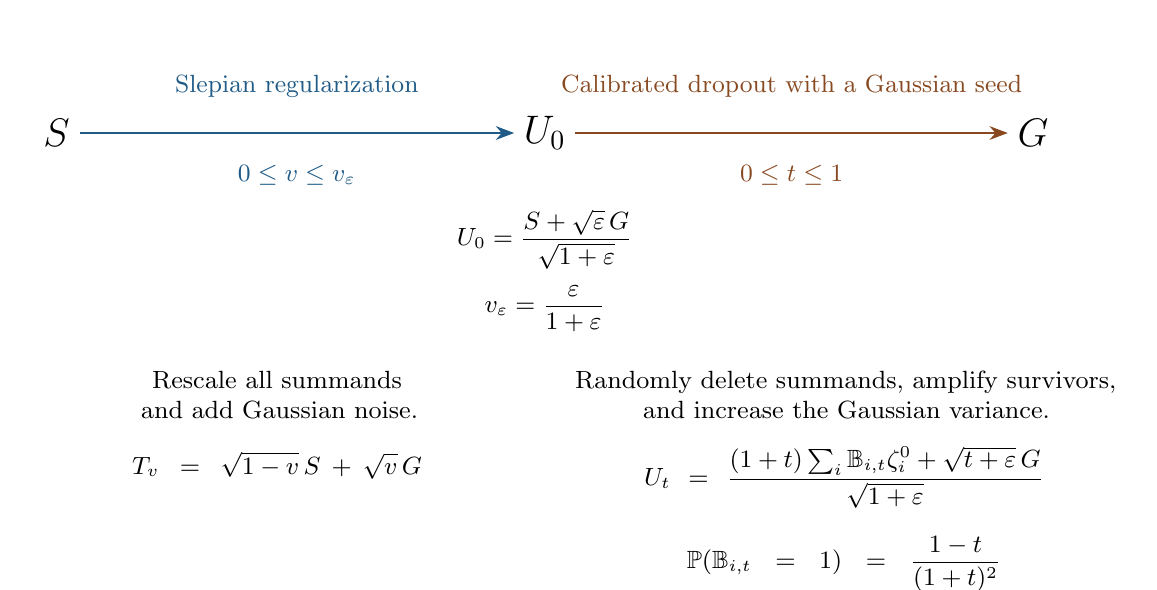
\begin{tikzpicture}[>=Stealth,font=\fontsize{9}{11}\selectfont]
\definecolor{seed}{RGB}{32,91,135}
\definecolor{drop}{RGB}{136,73,32}
\node[font=\Large] (S) at (0,0) {$S$};
\node[font=\Large] (U) at (6.2,0) {$U_0$};
\node[font=\Large] (G) at (12.4,0) {$G$};
\draw[->,thick,seed] (S) -- node[above=9pt,align=center] {Slepian regularization} node[below=8pt] {$0\le v\le v_\varepsilon$} (U);
\draw[->,thick,drop] (U) -- node[above=9pt,align=center] {Calibrated dropout with a Gaussian seed} node[below=8pt] {$0\le t\le1$} (G);
\node[anchor=north,align=center] at (6.2,-0.85) {$\displaystyle U_0=\frac{S+\sqrt\varepsilon\,G}{\sqrt{1+\varepsilon}}$
\\[5pt] $\displaystyle v_\varepsilon=\frac{\varepsilon}{1+\varepsilon}$};
\node[anchor=north,align=center,text width=6.1cm] at (2.8,-2.9) {Rescale all summands and add Gaussian noise.\\[9pt]
 $\displaystyle T_v=\sqrt{1-v}\,S+\sqrt v\,G$};
\node[anchor=north,align=center,text width=7.0cm] at (10,-2.9) {Randomly delete summands, amplify survivors,\\and increase the Gaussian variance.\\[9pt]
 $\displaystyle U_t=\frac{(1+t)\sum_i\mathbb B_{i,t}\zeta_i^0+\sqrt{t+\varepsilon}\,G}{\sqrt{1+\varepsilon}}$\\[9pt]
 $\displaystyle \mathbb P(\mathbb B_{i,t}=1)=\frac{1-t}{(1+t)^2}$};
\end{tikzpicture}
}
\caption{The comparison from \(S\) to \(G\) passes through the regularized
sum \(U_0\). The first stage follows \(T_v\) up to \(v_\varepsilon\),
and the second follows \(U_t\) from \(t=0\) to \(t=1\).}
\label{fig:two-stage-path}
\end{figure}

We first compare \(S\) with \(U_0\), and then \(U_0\) with \(G\).
For fixed thresholds, write
\[
 P_a(t)\coloneqq\E F_{a,h}(U_t),\qquad
 I_h\coloneqq\sup_a|\E F_{a,h}(S)-\E F_{a,h}(U_0)|.
\]
The quantity \(I_h\) measures the error from introducing the seed.

Consequently,
\begin{equation}
 M_h\le I_h+\sup_a\int_0^1|P_a'(t)|\,dt .
 \label{eq:roadmap}
\end{equation}
Here \(P_a'(t)\) is the rate at which the smoothed probability changes
at time \(t\). The small initial Gaussian component allows us to
integrate by parts twice on the second stage, including near \(t=0\).

\subsection{Controlling the comparison error}
\label{sec:outline-seeded}

To bound the integral in~\eqref{eq:roadmap}, let
\(K_3:=\sum_i\E(\zeta_i^0)^{\otimes3}\) denote the aggregate
third-moment tensor. Lemma~\ref{appx-an:lem:identity} separates its contribution
to the rate of change of \(P_a(t)\) from the fourth-order remainder,
\begin{equation}
 P_a'(t)=
 -\frac{t}{3(1+\varepsilon)^{3/2}}\,
       \E D^3F_{a,h}(U_t):K_3+R_{4,a,h}(t).
 \label{eq:path-summary}
\end{equation}
Here \(D^3F\) is the third derivative tensor, and the colon sums
products of corresponding tensor entries. The remainder \(R_{4,a,h}\) consists of fourth derivatives evaluated
at nearby points. As in~\cite[Lemmas~22--23]{GaoZhang}, we use the aggregate
covariance to sum pairs of directions before estimating the remaining
ones. Indeed, the identity covariance gives
\(\sum_i\E|(u\cdot\zeta_i^0)(w\cdot\zeta_i^0)|\le1\) for unit face
normals \(u,w\). Moving two derivatives from the logistic approximation
onto the Gaussian density by integration by parts contributes a
factor of order \((t+\varepsilon)^{-1}\). The matrix and surface estimates
in Appendix~\ref{appx-sec:support} preserve concentration near the
rectangle boundary in this calculation. This gains one power of the
smoothing width in the fourth-order remainder.

A larger seed improves this Gaussian estimate but increases the
initialization error. Choosing \(\varepsilon=Lh^2\) balances these
effects. The next proposition gives the estimates for both stages.
To state the initialization bound, write the corresponding Slepian
identity as
\[
 \frac{d}{dv}\E F_{a,h}(T_v)
 =-\frac{\sqrt{1-v}}4\E D^3F_{a,h}(T_v):K_3+R^0_{a,h}(v),
 \qquad 0<v<1.
\]
This defines its fourth-order remainder \(R^0_{a,h}\), whose integral
formula, like that of \(R_{4,a,h}\), is given by
Lemma~\ref{appx-an:lem:identity}.

\begin{proposition}[Initialization and seeded derivative estimates]
\label{an:prop:derivative}
Under~\eqref{eq:setup} and \eqref{eq:relative-moments}, there are absolute constants \(\mathsf A,C\)
such that, for \(h\ge\mathsf A\delta\), uniformly over
\(a\in\R^m\) and \(0<v<1\),
\begin{equation}
 |\E D^3F_{a,h}(T_v):K_3|\le\frac{Cs_3\sqrt L}{h^2},
 \qquad |R^0_{a,h}(v)|\le\frac{Cs_4\sqrt L}{h^3}.
 \label{eq:direct-initialization}
\end{equation}
If \(Lh^2<1/4\), choose \(\varepsilon=Lh^2\) in~\eqref{eq:path}.
Then
\begin{equation}
 I_h\le Cs_3 L^{3/2}+\frac{Cs_4L^{3/2}}h,
 \label{eq:initialization-bound}
\end{equation}
and, uniformly over \(a\in\R^m\) and \(0<t<1\),
\begin{equation}
 \begin{aligned}
 \left|\frac{t}{3(1+\varepsilon)^{3/2}}
          \E D^3F_{a,h}(U_t):K_3\right|
 &\le Cs_3 L^{3/2}\frac{t}{t+\varepsilon},\\
 |R_{4,a,h}(t)|&\le\frac{Cs_4L^{3/2}}{h(t+\varepsilon)}.
 \end{aligned}
 \label{eq:seeded-derivatives}
\end{equation}

\end{proposition}
\begin{proof}[Proof of Theorem~\ref{thm:unrestricted}]
Use admissible $s_3\le\delta$ (replace any supplied bound by its minimum with $\delta$). Take $h=\mathsf A\max\{\delta,\sqrt{s_4D_L}\}$ with $\mathsf A\ge1$ as in Proposition~\ref{an:prop:derivative}. If $Lh^2\ge1/4$, the right side of \eqref{eq:relative-unrestricted} is bounded below by a positive absolute constant before the factor $C$, and $\rho\le1$ suffices. Otherwise set $\varepsilon=Lh^2$. Integrating the cubic estimate costs $Cs_3L^{3/2}$, since $t/(t+\varepsilon)\le1$. Integrating the fourth-order estimate gives $\log(1+1/\varepsilon)$. Together with initialization and the smoothing estimate \eqref{eq:endpoint-min}, this yields
\[
 \rho\le C L^{3/2}\left[h+s_3+
 \frac{s_4}{h}\left\{1+\log\!\left(1+\frac1{Lh^2}\right)\right\}\right].
\]
Since $h\ge\delta$, the expression in braces is at most $C D_L$. The fourth-order term in brackets is therefore at most $C\sqrt{s_4D_L}$, and the boundary and cubic terms are at most $C(\delta+\sqrt{s_4D_L})$. This proves \eqref{eq:relative-unrestricted}. Taking $s_4=\delta^2$ and using $D_L\ge1$ gives \eqref{eq:unrestricted}.
\end{proof}

The surviving logarithm comes from integrating the fourth-order
remainder near the beginning of the second stage. The lower bounds in
Section~\ref{opt:section} account for the \(L^{3/2}\) factor and leave
open whether the additional logarithm is necessary.

\section{Polynomial moment envelopes}\label{sec:poly}

We now allow occasional observations larger than any fixed envelope.
Their contribution depends on the size of the largest absolute
coordinate in a row and on how often that size is attained. A moment
bound on the row maximum controls both. Two arguments give complementary bounds. A
conditional-truncation argument transfers the bounded-summand theorem
to every envelope moment of order greater than two. When coordinate
fourth moments are also controlled, a Bennett inequality improves the
polynomial-moment bound of Chernozhukov, Chetverikov, Kato, and
Koike~\cite{CCKK2022}. The comparison between these bounds depends on
both the moment order and the size of the moment parameter.

As in Corollary~\ref{cor:observations}, let \(W_n:=n^{-1/2}\sum_iX_i\)
for independent centered observations satisfying
\(n^{-1}\sum_i\E X_{ij}^2=1\) for each \(j\), and let \(Z_n\) be its matching Gaussian vector. We write
\(W=W_n\), \(Z=Z_n\), and retain \(L=\log(ep)\).
For \(q>2\) and \(B\ge1\), let \(\mathcal E_q(B,p)\) denote the class
of such arrays satisfying
\begin{equation}
 \max_{i\le n}\E\norm{X_i}_\infty^q\le B^q.
 \label{poly:envelope}
\end{equation}
The dependence of this class on \(n\) is suppressed. Condition
\eqref{poly:envelope} controls the \emph{random envelope}
\(\norm{X_i}_\infty\), rather than only the moments of individual
coordinates. In particular, it accounts for the possibility that a
large coordinate occurs at a different location in each observation.
The covariance may be singular, and distinct coordinates may coincide.

The rate contributed by this envelope condition is conveniently written
as
\begin{equation}
 \alpha_q:=\frac12-\frac1q,\qquad
 V_q:=Bn^{-\alpha_q}L^{1+\alpha_q}.
 \label{poly:rates}
\end{equation}
Here \(\alpha_q>0\), and constants indexed by \(q\) may depend on the
fixed moment order. Our results are not uniform as \(q\) approaches two
or infinity.

\subsection{Transfer from bounded observations}\label{poly:transfer-sec}

Truncating all rows and paying the probability that any row changes
loses information about the size of the exceptional observations.
Instead, we condition on which rows are exceptional. Given this
information, the remaining rows are independent and bounded, and the
exceptional part can be treated as a random shift. The bounded-summand
theorem and Gaussian anti-concentration then control the two parts.

\begin{theorem}[Polynomial envelope transfer]\label{poly:transfer}
For every fixed \(q>2\), there is a constant \(C_q\) such that, for
every array in \(\mathcal E_q(B,p)\),
\begin{equation}
 \rh(W,Z)\le C_q\min\{1,V_q\{\log(en)\}^{\alpha_q}\}.
 \label{poly:transfer-bound}
\end{equation}
Only the unit marginal variances and the envelope condition
\eqref{poly:envelope} are required.
\end{theorem}

Appendix~\ref{app:conditional} chooses the truncation threshold by
balancing the approximation error for bounded observations against the
variance discarded in the tails. The extra logarithm in
\eqref{poly:transfer-bound} comes from the bounded-observation theorem.
If Conjecture~\ref{conj:sharp-unrestricted} holds, the same argument
gives \(C_q\min\{1,V_q\}\) under the envelope condition alone.

\subsection{A refinement under coordinate fourth moments}\label{poly:bennett-sec}

Coordinate fourth moments can be substantially smaller than the fourth
moment of the random envelope. Retaining that distinction improves the
bound when the largest observations are spread sparsely over coordinates.
Let \(\mathcal C_q(B,p)\) be the subclass of \(\mathcal E_q(B,p)\)
that also satisfies
\begin{equation}
 \max_{j\le p}\frac1n\sum_{i=1}^n\E X_{ij}^4\le B^2.
 \label{poly:fourth}
\end{equation}
Condition \eqref{poly:fourth} is imposed even when \(2<q<4\).
At \(q=4\), the coordinate and envelope budgets are respectively
\(B^2\) and \(B^4\).

Under these conditions, the polynomial-moment bound of Chernozhukov,
Chetverikov, Kato, and Koike~\cite[Theorem~2.5]{CCKK2022} gives
\(\rh(W,Z)\le C_q\min\{1,U+V_q\}\). To obtain its rectangle form,
apply their lower-orthant bound to \((X_i,-X_i)\). The moment budgets
are preserved, and \(\log(2p)\) is comparable to \(L\). Put
\begin{equation}
 U:=\left(\frac{B^2L^5}{n}\right)^{1/4},\qquad
 \mathcal K_q:=\left(\frac{V_q}{U}\right)^2
     =B\left(\frac nL\right)^{2/q-1/2},\qquad
 \mathcal{L}_q:=\log(e+\mathcal K_q).
 \label{poly:bennett-parameters}
\end{equation}
Here \(\mathcal K_q\) compares the two contributions in the CCKK bound.
When \(\mathcal K_q\) is large, Bennett's inequality reduces the envelope
contribution by a power of the logarithmic factor \(\mathcal{L}_q\).

\begin{theorem}[Bennett refinement]\label{poly:bennett}
For every fixed \(q>2\), there is a constant \(C_q\) such that, for
every array in \(\mathcal C_q(B,p)\),
\begin{equation}
 \rh(W,Z)\le C_q\min\left\{1,
 U+\frac{V_q}{\mathcal{L}_q^{1-1/q}}\right\}.
 \label{poly:bennett-bound}
\end{equation}
The observations need not be identically distributed or symmetric.
\end{theorem}

The proof replaces the maximal inequality for large exchangeable-pair
increments in the CCKK argument by a Bennett bound. Its variance estimate
uses both \eqref{poly:envelope} and \eqref{poly:fourth}.
Appendix~\ref{app:bennett} gives the proof, following the argument
in~\cite{BennettNote}. Basu and Kuchibhotla use a related truncation
argument for maxima of independent sums~\cite[Proposition~4.2]{BK2025}.

The two upper bounds apply simultaneously on \(\mathcal C_q(B,p)\).
Consequently,
\begin{equation}
 \sup_{\mathcal C_q(B,p)}\rh(W,Z)
 \le C_q\min\left\{1,
 U+\frac{V_q}{\mathcal{L}_q^{1-1/q}},\ V_q\{\log(en)\}^{\alpha_q}\right\}.
 \label{poly:combined}
\end{equation}
This formulation is useful when \(B\) varies with \(n\), since \(\mathcal K_q\) tracks the joint
effect of \(B\) and \(q\).
Table~\ref{poly:summary} distinguishes the two proof routes and the
sharpness conclusions established for each. In particular, the
conditional-truncation result retains a logarithmic gap when \(q>4\)
and \(B\) is fixed.

\begin{table}[htbp]
\centering
\small
\renewcommand{\arraystretch}{1.15}
\begin{tabularx}{\textwidth}{@{}>{\raggedright\arraybackslash}p{0.20\textwidth}
 >{\raggedright\arraybackslash}p{0.28\textwidth}
 >{\raggedright\arraybackslash}X@{}}
\toprule
Result and upper rate & Proof route & Sharpness established\\
\midrule
Theorem~\ref{poly:transfer}\newline
Appendix~\ref{app:conditional}\newline
\(V_q\{\log(en)\}^{\alpha_q}\)
& Conditional truncation, followed by the bounded-summand theorem and
Gaussian anti-concentration.
& For fixed \(B\ge2\) and \(q>4\), the lower rate is \(V_q\) in
Theorem~\ref{lower:dense}. The remaining gap is
\(\{\log(en)\}^{\alpha_q}\), and its necessity is unresolved.\\[0.6em]
Theorem~\ref{poly:bennett}\newline
Appendix~\ref{app:bennett}\newline
\(U+V_q/\mathcal{L}_q^{1-1/q}\)
& The CCKK Stein estimate, a variance bound using both moment budgets,
and a Bennett inequality for large increments.
& Matching rates in the large-\(\mathcal K_q\) regime of
Theorem~\ref{lower:sparse}, and for fixed \(B\ge2\) at \(q=4\)
by Theorem~\ref{opt:q4-lower}. The term \(U\) remains when \(q>4\)
and \(B\) is fixed.\\
\bottomrule
\end{tabularx}
\caption{Upper bounds, proof methods, and scope of sharpness.
Constants are suppressed and both upper bounds are capped at 1.
The comparisons use the dimension and vanishing-rate conditions of
the cited results in Section~\ref{opt:section}.}
\label{poly:summary}
\end{table}

\subsection{The transition at four moments}\label{poly:transition}

For fixed \(B\) and \(n/L\to\infty\), the three ranges of \(q\)
have different interpretations. If \(2<q<4\), then \(\mathcal K_q\to\infty\)
and
\[
 \frac{V_q/\mathcal{L}_q^{1-1/q}}{U}
   =\frac{\sqrt{\mathcal K_q}}{\mathcal{L}_q^{1-1/q}}\longrightarrow\infty.
\]
The Bennett bound therefore has order \(V_q/\mathcal{L}_q^{1-1/q}\).
The sparse construction in Theorem~\ref{lower:sparse} matches this
order when \(\log \mathcal K_q=o(L)\) and the rate tends to zero.

At \(q=4\), \(\mathcal K_4=B\), and the first term is absorbed uniformly in
\(B\ge1\), because \(\{\log(e+B)\}^{3/4}/\sqrt B\) is bounded.
Thus Theorem~\ref{poly:bennett} gives
\begin{equation}
 \rh(W,Z)\le C\min\left\{1,
 \frac{Bn^{-1/4}L^{5/4}}{\{\log(e+B)\}^{3/4}}\right\}.
 \label{poly:q4}
\end{equation}
The fixed-envelope lower bound and the sparse growing-envelope lower
bound in Section~\ref{opt:section} identify the order in their respective
dimension regimes.

If \(q>4\) and \(B\) is fixed, then \(\mathcal K_q\to0\). The CCKK and
Bennett bounds retain the term \(U\), whereas Theorem
\ref{poly:transfer} gives \(V_q\{\log(en)\}^{\alpha_q}\). In particular, for
\(p\asymp n^a\), where \(a>0\) is fixed, the latter rate is
\[
 O_{q,B,a}\!\left(n^{-\alpha_q}(\log n)^{1+2\alpha_q}\right).
\]
Since \(\alpha_q>1/4\), this improves the power of \(n\) in the CCKK
bound. Theorem~\ref{lower:dense} supplies the lower rate \(V_q\), so
the remaining gap is at most \(\{\log(en)\}^{\alpha_q}\). For example, at
\(q=6\) the lower rate is \(Bn^{-1/3}L^{4/3}\), and the upper rate
is this quantity times \(\{\log(en)\}^{1/3}\). We do not assert that this
remaining logarithm is necessary.

\section{Sharpness of the bounds}\label{opt:section}

Two mechanisms explain the lower bounds. With independent coordinates,
a small error in each scalar tail can accumulate at the threshold of
the maximum. With strongly dependent coordinates, a small independent
shift changes the maximum by an amount that its concentrated
distribution can detect. The second construction works even under
central symmetry and, with a change of amplitude, under a polynomial
moment envelope. Appendix~\ref{app:sharpness-proofs} gives the proofs.

Table~\ref{opt:tab:rates} compares these examples with the upper bounds
in Corollary~\ref{cor:observations} and Section~\ref{sec:poly}.
At \(q=4\) the rates match even under central symmetry. For bounded
observations and for fixed \(B\) with \(q>4\), a logarithmic gap remains.

\begin{table}[!htb]
\centering
\caption{Upper and lower bounds for the Kolmogorov distance over rectangles
with unrestricted covariance. A rate centered across the two columns gives
both bounds up to constants.}
\label{opt:tab:rates}
\vspace{3pt}
\small
\setlength{\tabcolsep}{3pt}
\begin{tabular*}{\linewidth}{@{\extracolsep{\fill}}lcc@{}}
\toprule
Observations & Lower bound & Upper bound\\
\midrule
\shortstack[l]{Bounded by \(B\)\\Theorem~\ref{opt:skew-lower}}
& \(\displaystyle\frac{B(\log p)^{3/2}}{\sqrt n}\)
& \(\displaystyle\frac{B(\log p)^{3/2}}{\sqrt n}
   \sqrt{\log\!\left(e+\frac{\sqrt n}{B\sqrt{\log p}}\right)}\)\\
\addlinespace[4pt]
\shortstack[l]{Bounded by \(2\), centrally\\symmetric (Theorem~\ref{opt:symmetric-lower})}
& \(\displaystyle\frac{(\log p)^{3/2}}{\sqrt n}\)
& \(\displaystyle\frac{(\log p)^{3/2}}{\sqrt n}
   \sqrt{\log\!\left(e+\sqrt{n/\log p}\right)}\)\\
\midrule
\shortstack[l]{\(q=4\), fixed \(B\)\\Theorem~\ref{opt:q4-lower}}
& \multicolumn{2}{c@{}}{\(\displaystyle\frac{(\log p)^{5/4}}{n^{1/4}}\)}\\
\addlinespace[4pt]
\shortstack[l]{\(q=4\), \(B\to\infty\),\\\(\log B=o(\log p)\) (Theorem~\ref{opt:q4-growing})}
& \multicolumn{2}{c@{}}{\(\displaystyle
  \frac{B(\log p)^{5/4}}{n^{1/4}\{\log(e+B)\}^{3/4}}\)}\\
\addlinespace[4pt]
\shortstack[l]{\(q>4\), fixed \(B\)\\Theorem~\ref{lower:dense}}
& \(\displaystyle\frac{B(\log p)^{3/2-1/q}}{n^{1/2-1/q}}\)
& \(\displaystyle\frac{B(\log p)^{3/2-1/q}\{\log(en)\}^{1/2-1/q}}
                         {n^{1/2-1/q}}\)\\
\addlinespace[4pt]
\shortstack[l]{\(2<q<4\), fixed \(B\),\\\(\log n=o(\log p)\) (Theorem~\ref{lower:sparse})}
& \multicolumn{2}{c@{}}{\(\displaystyle
  \frac{(\log p)^{3/2-1/q}}
       {n^{1/2-1/q}\{\log(e+n/\log p)\}^{1-1/q}}\)}\\
\addlinespace[4pt]
\shortstack[l]{\(q>2\), sparse regime\\Theorem~\ref{lower:sparse}}
& \multicolumn{2}{c@{}}{\(\displaystyle
  \frac{B(\log p)^{3/2-1/q}}
       {n^{1/2-1/q}\{\log(e+B(n/\log p)^{2/q-1/2})\}^{1-1/q}}\)}\\
\bottomrule
\end{tabular*}
\par\medskip
\begin{minipage}{\linewidth}\small
Here \(n\) is the sample size, \(p\) is the dimension, and \(B\ge2\).
Each comparison assumes \(p\to\infty\) and that the displayed lower rate
tends to zero. The examples in Theorems~\ref{opt:symmetric-lower}--\ref{lower:sparse}
use \(p=m^2\) and are centrally symmetric. In the polynomial rows, \(q\) is
fixed, and both the envelope bound~\eqref{poly:envelope} and the coordinate
fourth-moment bound~\eqref{poly:fourth} hold. Constants may depend on \(q\)
and, in fixed-envelope rows, on \(B\). In the last row, \(B\) may vary with
\(n\), and the sparse regime requires
\(B(n/\log p)^{2/q-1/2}\to\infty\) and
\(\log\!\bigl(B(n/\log p)^{2/q-1/2}\bigr)=o(\log p)\).
\end{minipage}
\end{table}

\subsection{Bounded observations}
We first vary a skewed two-point distribution to see how the error
depends jointly on the envelope \(B_n\) and the dimension. The
example builds on~\cite[Proposition~2.1]{CCK}.

\begin{theorem}[Lower scale]\label{opt:skew-lower}
Suppose \(p_n\to\infty\), \(B_n\ge2\), and
\(r_n\coloneqq B_n(\log p_n)^{3/2}/\sqrt n\to0\). There are i.i.d.
centered observations with independent coordinates, covariance
\(I_{p_n}\), and envelope \(B_n\), for which
\begin{equation}
 \liminf_n\frac{\rh(W_n,Z_n)}{r_n}\ge\frac{\sqrt2}{4e}.
 \label{opt:lower-constant}
\end{equation}
Here \(W_n\coloneqq n^{-1/2}\sum_iX_{n,i}\),
\(Z_n\sim N(0,I_{p_n})\), and the envelope is attained.
\end{theorem}

For comparison, a common rare activation across many coordinates can
produce the same lower scale when all third moments vanish.
In describing these examples we use the \emph{correlation gap}
\(c_n:=1-\max_{j\ne k}|\operatorname{Corr}(W_{n,j},W_{n,k})|\)
to quantify how close a pair of distinct coordinates comes to perfect
dependence.

\begin{theorem}[Centrally symmetric lower bound]\label{opt:symmetric-lower}
Let \(m_n\ge2\) be integers such that \(m_n\to\infty\) and
\((\log m_n)^3/n\to0\). Put
\[
 p_n\coloneqq m_n^2,\qquad \delta_n\coloneqq\frac2{\sqrt n},
 \qquad L_n\coloneqq\log(ep_n).
\]
For all sufficiently large \(n\), there are i.i.d.\ centered vectors
\(X_{n,i}\in\R^{p_n}\), \(1\le i\le n\), with centrally symmetric
law, unit marginal variances, and \(\norm{X_{n,i}}_\infty\le2\).
Their covariance \(\Sigma_n\) has rank \(2m_n-1\) and correlation
gap \(c_n=(\log m_n)/(2n)\). The normalized sum
\(W_n\coloneqq n^{-1/2}\sum_{i=1}^nX_{n,i}\) and its Gaussian
counterpart \(Z_n\sim N(0,\Sigma_n)\) satisfy
\[
 \liminf_{n\to\infty}
 \frac{\rh(W_n,Z_n)}{\delta_nL_n^{3/2}}\ge\frac1{8e}.
\]
\end{theorem}

Here the rank grows much more slowly than the number of coordinates.
Appendix~\ref{app:symmetric-lower} proves the theorem using a
modification of the common activation construction
in~\cite[Proposition~E.1]{FKLZ}.

The lower scale can also be attained with gap exactly zero. Append
a copy of the first coordinate to every observation and to the Gaussian
vector. A rectangle in the enlarged space tests the first coordinate
against the intersection of two intervals, so its inverse image is a
rectangle or the empty set. Conversely, every original rectangle is
obtained by leaving the added coordinate unrestricted. Thus duplication
preserves the discrepancy exactly, as well as symmetry and both
coordinate and maximum-norm moment bounds. Replacing \(p_n\) by
\(p_n+1\) leaves the asymptotic logarithmic factor unchanged.

\subsection{Fourth-moment envelopes}\label{opt:q4-comparison}

Under the fourth-moment conditions of Section~\ref{sec:poly}, the
coordinate bound controls the variance of rare increments, and the
envelope bound limits their size. We now show that symmetric observations in the class
\(\mathcal C_4(B,p)\) defined by
\eqref{poly:envelope} and~\eqref{poly:fourth} attain the rate
in~\eqref{poly:q4}. We start with a fixed \(B\).

\begin{theorem}[Fourth-moment lower bound]\label{opt:q4-lower}
Let \(m_n\to\infty\) be integers, put \(p_n:=m_n^2\) and
\(L_n:=\log(ep_n)\), and suppose
\(r_{n,4}:=n^{-1/4}L_n^{5/4}\to0\).
For all sufficiently large \(n\), there are i.i.d.\ centrally
symmetric observations in \(\mathcal C_4(2,p_n)\) whose covariance
has rank \(2m_n-1\) and correlation gap
\(c_n=\sqrt{(\log m_n)/(2n)}\), such that
\begin{equation}
 \liminf_{n\to\infty}
 \frac{\rh(W_n,Z_n)}{r_{n,4}}\ge\frac1{2\sqrt2\,e}.
 \label{opt:eq:q4-lower}
\end{equation}
Consequently, for every fixed \(B\ge2\), along these dimension sequences,
\begin{equation}
 \sup_{\mathcal C_4(B,p_n)}\rh(W_n,Z_n)
 \asymp_B n^{-1/4}L_n^{5/4}.
 \label{lower:q4-fixed}
\end{equation}
The same conclusion holds if the supremum is restricted to centrally
symmetric observations.
\end{theorem}

This confirms our conjecture that the \(n^{-1/4}\) rate in the Gaussian
approximation bound of Chernozhukov, Chetverikov, Kato, and
Koike~\cite[Theorem~2.5]{CCKK2022} is sharp when \(q=4\).
For fixed \(B\ge2\), the lower bound also matches the dimension factor
\(L_n^{5/4}\), even for centrally symmetric observations.
Appendix~\ref{app:symmetric-lower} obtains this example from the
bounded symmetric construction by increasing the amplitude of its rare
component.

When \(B\) grows, the upper bound in~\eqref{poly:q4} contains a
logarithm of \(B\) in the denominator. The next example shows that even
this logarithmic improvement is sharp. Independent masks across
coordinates allow a large observation to use its envelope budget while
remaining rare in each coordinate.

\begin{theorem}[Growing fourth-moment envelope]\label{opt:q4-growing}
Let \(B_n\ge2\) tend to infinity and let \(m_n\to\infty\) be integers.
Set
\[
 p_n:=m_n^2,\qquad \ell_n:=\log m_n,\qquad
 \Lambda_n:=\log(2B_n^2),\qquad
 r_{n,B}:=\frac{B_n\ell_n^{5/4}}{n^{1/4}\Lambda_n^{3/4}}.
\]
Suppose \(\Lambda_n=o(\ell_n)\) and \(r_{n,B}\to0\).
For all sufficiently large \(n\), there are i.i.d.\ centrally
symmetric observations in \(\mathcal C_4(B_n,p_n)\) such that
\begin{equation}
 \liminf_{n\to\infty}
 \frac{\rh(W_n,Z_n)}{r_{n,B}}\ge\frac1{4e}.
 \label{opt:eq:q4-growing}
\end{equation}
Their covariance has rank \(2m_n-1\) and correlation gap
\(c_n=\frac14\sqrt{\ell_n/(4n\Lambda_n)}\to0\).
\end{theorem}

Since \(L_n=1+2\ell_n\) and \(\Lambda_n\sim2\log B_n\), the lower
rate in Theorem~\ref{opt:q4-growing} agrees up to constants with
the upper rate in~\eqref{poly:q4}, including its dependence on \(B_n\).
Both fourth-moment examples have correlation gaps tending to zero.

\subsection{Polynomial envelopes beyond the fourth moment}

For \(q>4\), the envelope moment permits a rare amplitude whose
coordinate fourth-moment contribution tends to zero. The same unmasked construction as in
Theorem~\ref{opt:q4-lower} therefore suffices when \(B\) is fixed.

\begin{theorem}[Lower bound for fixed \(B\) and \(q>4\)]\label{lower:dense}
Fix \(q>4\) and \(B\ge2\). Let \(m_n\to\infty\) be integers, set
\(p_n:=m_n^2\), \(L_n:=\log(ep_n)\), and suppose
\(V_{n,q}:=Bn^{-\alpha_q}L_n^{1+\alpha_q}\to0\).
For all sufficiently large \(n\), there are i.i.d.\ centrally symmetric
observations in \(\mathcal C_q(B,p_n)\) such that
\begin{equation}
 \liminf_{n\to\infty}\frac{\rh(W_n,Z_n)}{V_{n,q}}>0.
 \label{lower:dense-rate}
\end{equation}
Their covariance has rank \(2m_n-1\), and their correlation gap tends
to zero. Consequently, along these dimension sequences,
\[
 c_{q,B}V_{n,q}
 \le\sup_{\mathcal C_q(B,p_n)}\rh(W_n,Z_n)
 \le C_qV_{n,q}\{\log(en)\}^{\alpha_q}.
\]
\end{theorem}

The lower bound has the same power of \(n\) as the transfer bound in
Theorem~\ref{poly:transfer}. For fixed \(B\) and \(q>4\), the remaining
factor is at most \(\{\log(en)\}^{\alpha_q}\).

\subsection{Sparse observations and the Bennett denominator}

When \(\mathcal K_q\) is large, a dense rare component would spend too much of
the coordinate fourth-moment budget. Independent masks across coordinates
reduce that expenditure. The price is that more coordinates are needed
to find one that captures all active positive spikes. This price produces
the logarithm in the denominator of the upper bound.

\begin{theorem}[Sparse polynomial-moment lower bound]\label{lower:sparse}
Fix \(q>2\). Let \(B_n\ge2\), let \(m_n\to\infty\) be integers,
and put \(p_n:=m_n^2\), \(L_n:=\log(ep_n)\), and
\[
 \mathcal K_{n,q}:=B_n(n/L_n)^{2/q-1/2},\qquad
 R_{n,q}:=\frac{B_n n^{-\alpha_q}L_n^{1+\alpha_q}}
                    {\{\log(e+\mathcal K_{n,q})\}^{1-1/q}}.
\]
Suppose
\begin{equation}
 \mathcal K_{n,q}\longrightarrow\infty,\qquad
 \log \mathcal K_{n,q}=o(L_n),\qquad R_{n,q}\longrightarrow0.
 \label{lower:sparse-regime}
\end{equation}
For all sufficiently large \(n\), there are i.i.d.\ centrally symmetric
observations in \(\mathcal C_q(B_n,p_n)\) with covariance rank
\(2m_n-1\) and correlation gap tending to zero, such that
\begin{equation}
 \rh(W_n,Z_n)\ge c_qR_{n,q}.
 \label{lower:sparse-rate}
\end{equation}
Together with Theorem~\ref{poly:bennett}, this gives
\(\sup_{\mathcal C_q(B_n,p_n)}\rh(W_n,Z_n)\asymp_q R_{n,q}\)
under \eqref{lower:sparse-regime}, including when the supremum is
restricted to centrally symmetric observations.
\end{theorem}

For fixed \(B\) and \(2<q<4\), the extra dimension condition in
\eqref{lower:sparse-regime} is satisfied, for example, when
\(\log n=o(L_n)\). At \(q=4\), it reduces to the growing-envelope
conditions \(B_n\to\infty\) and \(\log B_n=o(L_n)\), together
with \(R_{n,4}\to0\). The theorem also applies to \(q>4\) when
\(B_n\) grows sufficiently quickly that \(\mathcal K_{n,q}\to\infty\).
It does not establish a minimax formula for all smaller dimensions
or every intermediate sequence of \(\mathcal K_{n,q}\).

\section{Remaining questions and formal verification}\label{sec:discussion}

\subsection{The logarithmic gap for bounded observations}

For bounded observations with unrestricted covariance, our upper and
lower bounds differ by an additional logarithmic factor. We conjecture
that this factor can be removed, giving an upper bound that matches
the examples above uniformly over covariance matrices.
\begin{conjecture}[Sharp rectangle approximation under unrestricted covariance]
\label{conj:sharp-unrestricted}
Under~\eqref{eq:setup}, there is an absolute constant \(C\) such that
\[
 \rh(W,Z)\le C\min\{1,\delta L^{3/2}\},\qquad L=\log(ep),
\]
uniformly in \(n,p,\delta\) and \(\Sigma\), including singular \(\Sigma\).
\end{conjecture}

The lower bounds show that the dimension dependence in this conjecture
cannot generally be improved, even for centrally symmetric observations.


Theorem~\ref{thm:unrestricted} proves the conjectured rate for arrays with $s_4D_L\lesssim\delta^2$. A bound on the cumulative comparison error without the extra logarithm for all bounded arrays would give the full conjecture
and sharpen the polynomial transfer in Subsection~\ref{poly:transfer-sec}.

\subsection{Lean certification of the main result}\label{sec:lean-certification}

A separate proof checked in Lean establishes the envelope specialization \eqref{eq:unrestricted} of Theorem~\ref{thm:unrestricted}.
The formal development also establishes the sub-exponential rectangle
bound in Corollary~\ref{cor:subexponential} and the lower bound for
skewed bounded observations in Theorem~\ref{opt:skew-lower}. The
\href{https://github.com/VC2015/HDCLTs/blob/bbf1ab99c733a398c181ca8c9f5a243a41f258c6/verification/2026-10-21-companion-results/README.md}{October 2026 verification record}
links the Lean proofs, their axiom audits, and the correspondence between
the formal statements and the manuscript. The relative-moment refinement \eqref{eq:relative-unrestricted}, its interpolation proof, the polynomial-moment results, the symmetric lower
bounds, and the polyhedral extension await formal verification.

\begin{thebibliography}{99}
\setlength{\itemsep}{1pt}
\phantomsection
\addcontentsline{toc}{section}{References}
\bibitem{AL}
P.~M. Aronow and P. Lopatto (2026).
\emph{Optimal central limit theorem for bounded random variables in high dimensions}.
Manuscript, arXiv:2609.07067v1.
\url{https://arxiv.org/abs/2609.07067v1}.

\bibitem{CCK2013}
V. Chernozhukov, D. Chetverikov, and K. Kato (2013).
\emph{Gaussian approximations and multiplier bootstrap for maxima of
sums of high-dimensional random vectors}.
The Annals of Statistics \textbf{41}(6), 2786--2819.
\href{https://doi.org/10.1214/13-AOS1161}{doi:10.1214/13-AOS1161}.

\bibitem{CCK2017}
V. Chernozhukov, D. Chetverikov, and K. Kato (2017).
\emph{Central limit theorems and bootstrap in high dimensions}.
The Annals of Probability \textbf{45}(4), 2309--2352.
\href{https://doi.org/10.1214/16-AOP1113}{doi:10.1214/16-AOP1113}.

\bibitem{CCKK2022}
V. Chernozhukov, D. Chetverikov, K. Kato, and Y. Koike (2022).
\emph{Improved central limit theorem and bootstrap approximations in
high dimensions}. The Annals of Statistics \textbf{50}(5), 2562--2586.
\href{https://doi.org/10.1214/22-AOS2193}{doi:10.1214/22-AOS2193}.

\bibitem{CCKK2023}
V. Chernozhukov, D. Chetverikov, K. Kato, and Y. Koike (2023).
\emph{High-dimensional data bootstrap}.
Annual Review of Statistics and Its Application \textbf{10}, 427--449.
Working version: arXiv:2205.09691.
\url{https://arxiv.org/abs/2205.09691}.

\bibitem{Local}
V. Chernozhukov, D. Chetverikov, K. Kato, and Y. Koike,
with AI collaborators (2026).
\emph{High-dimensional Gaussian approximation over rectangles under
local nondegeneracy}. Companion working manuscript, 21 October 2026.

\bibitem{CCK}
V. Chernozhukov, D. Chetverikov, and Y. Koike (2023).
\emph{Nearly optimal central limit theorem and bootstrap approximations
in high dimensions}.
The Annals of Applied Probability \textbf{33}(3), 2374--2425.
\href{https://doi.org/10.1214/22-AAP1870}{doi:10.1214/22-AAP1870}.
Working version: arXiv:2012.09513v2, May 12, 2021.
\url{https://arxiv.org/abs/2012.09513v2}.

\bibitem{FKLZ}
X. Fang, Y. Koike, S.-H. Liu, and Y.-K. Zhao (2026).
\emph{High-dimensional central limit theorems by Stein's method in
the degenerate case}. The Annals of Applied Probability, to appear.
arXiv:2305.17365.
\href{https://research.cuhk.edu.hk/en/publications/high-dimensional-central-limit-theorems-by-steins-method-in-the-d/}{Accepted manuscript (2026)}.

\bibitem{GaoZhang}
Z. Gao and W. Zhang (2026).
\emph{Cubic-root Gaussian approximation under unrestricted covariance}.
arXiv:2608.30221v1, 31 August 2026.
\url{https://arxiv.org/abs/2608.30221v1}.

\bibitem{Kane}
D.~M. Kane (2014).
\emph{The average sensitivity of an intersection of half spaces}.
Research in the Mathematical Sciences \textbf{1}, Article~13.
\href{https://doi.org/10.1186/s40687-014-0013-6}{doi:10.1186/s40687-014-0013-6}.
Working version: arXiv:1309.2987v3.
\url{https://arxiv.org/abs/1309.2987v3}.

\bibitem{McFadden1989}
D. McFadden (1989).
\emph{A method of simulated moments for estimation of discrete
response models without numerical integration}.
Econometrica \textbf{57}(5), 995--1026.
\href{https://doi.org/10.2307/1913621}{doi:10.2307/1913621}.

\bibitem{OST}
R. O'Donnell, R.~A. Servedio, and L.-Y. Tan (2019).
Fooling polytopes.
In \emph{Proceedings of the 51st Annual ACM SIGACT Symposium on
Theory of Computing}, 614--625.
\href{https://doi.org/10.1145/3313276.3316321}{doi:10.1145/3313276.3316321}.

\bibitem{Prekopa1973}
A.~Pr\'ekopa (1973).
\emph{On logarithmic concave measures and functions}.
Acta Scientiarum Mathematicarum (Szeged) \textbf{34}, 335--343.
\url{https://rutcor.rutgers.edu/Prekopa/pdf/SCIENT2.pdf}.

\bibitem{Dropout2014}
N. Srivastava, G. Hinton, A. Krizhevsky, I. Sutskever, and
R. Salakhutdinov (2014).
\emph{Dropout: A simple way to prevent neural networks from overfitting}.
Journal of Machine Learning Research \textbf{15}(56), 1929--1958.
\url{https://www.jmlr.org/papers/v15/srivastava14a.html}.

\bibitem{Bhatia1997}
R. Bhatia (1997).
\emph{Matrix Analysis}.
Graduate Texts in Mathematics \textbf{169}. Springer, New York.
\href{https://doi.org/10.1007/978-1-4612-0653-8}{doi:10.1007/978-1-4612-0653-8}.

\bibitem{Comtet1974}
L. Comtet (1974).
\emph{Advanced Combinatorics: The Art of Finite and Infinite Expansions}.
Reidel, Dordrecht.
\href{https://doi.org/10.1007/978-94-010-2196-8}{doi:10.1007/978-94-010-2196-8}.

\bibitem{CoverThomas2006}
T. M. Cover and J. A. Thomas (2006).
\emph{Elements of Information Theory}, 2nd edition.
Wiley, Hoboken, NJ.

\bibitem{EvansGariepy2015}
L. C. Evans and R. F. Gariepy (2015).
\emph{Measure Theory and Fine Properties of Functions}, revised edition.
CRC Press, Boca Raton, FL.

\bibitem{Folland1999}
G. B. Folland (1999).
\emph{Real Analysis: Modern Techniques and Their Applications}, 2nd edition.
Wiley, New York.

\bibitem{RockafellarWets1998}
R. T. Rockafellar and R. J.-B. Wets (1998).
\emph{Variational Analysis}.
Grundlehren der mathematischen Wissenschaften \textbf{317}.
Springer, Berlin.
\href{https://doi.org/10.1007/978-3-642-02431-3}{doi:10.1007/978-3-642-02431-3}.

\bibitem{Stein1981}
C. M. Stein (1981).
\emph{Estimation of the mean of a multivariate normal distribution}.
The Annals of Statistics \textbf{9}(6), 1135--1151.
\href{https://doi.org/10.1214/aos/1176345632}{doi:10.1214/aos/1176345632}.

\bibitem{Ziegler1995}
G. M. Ziegler (1995).
\emph{Lectures on Polytopes}.
Graduate Texts in Mathematics \textbf{152}. Springer, New York.
\href{https://doi.org/10.1007/978-1-4613-8431-1}{doi:10.1007/978-1-4613-8431-1}.

\bibitem{BLM2013}
S. Boucheron, G. Lugosi, and P. Massart (2013).
\emph{Concentration Inequalities: A Nonasymptotic Theory of Independence}.
Oxford University Press, Oxford.
\href{https://doi.org/10.1093/acprof:oso/9780199535255.001.0001}{\nolinkurl{doi:10.1093/acprof:oso/9780199535255.001.0001}}.

\bibitem{Berry1941}
A. C. Berry (1941).
\emph{The accuracy of the Gaussian approximation to the sum of independent variates}.
Transactions of the American Mathematical Society \textbf{49}(1), 122--136.
\href{https://doi.org/10.1090/S0002-9947-1941-0003498-3}{doi:10.1090/S0002-9947-1941-0003498-3}.

\bibitem{BrascampLieb1976}
H. J. Brascamp and E. H. Lieb (1976).
\emph{On extensions of the Brunn--Minkowski and Pr\'ekopa--Leindler
theorems, including inequalities for log concave functions, and with
an application to the diffusion equation}.
Journal of Functional Analysis \textbf{22}(4), 366--389.
\href{https://doi.org/10.1016/0022-1236(76)90004-5}{doi:10.1016/0022-1236(76)90004-5}.

\bibitem{Rockafellar1970}
R. T. Rockafellar (1970).
\emph{Convex Analysis}.
Princeton Mathematical Series \textbf{28}.
Princeton University Press, Princeton, NJ.

\bibitem{Nazarov2003}
F. Nazarov (2003).
\emph{On the maximal perimeter of a convex set in \(\R^n\)
with respect to a Gaussian measure}.
In V. D. Milman and G. Schechtman (eds.),
\emph{Geometric Aspects of Functional Analysis (2001--2002)},
Lecture Notes in Mathematics \textbf{1807}, 169--187.
Springer, Berlin.

\bibitem{CCK17N}
V. Chernozhukov, D. Chetverikov, and K. Kato (2017).
\emph{Detailed proof of Nazarov's inequality}.
arXiv:1711.10696.
\url{https://arxiv.org/abs/1711.10696}.

\bibitem{BoydVandenberghe2004}
S. Boyd and L. Vandenberghe (2004).
\emph{Convex Optimization}.
Cambridge University Press, Cambridge.
\url{https://web.stanford.edu/~boyd/cvxbook/bv_cvxbook.pdf}.

\bibitem{Nourdin2012}
I. Nourdin (2012).
\emph{Lectures on Gaussian approximations with Malliavin calculus}.
Lecture notes, arXiv:1203.4147v3.
\url{https://arxiv.org/abs/1203.4147v3}.

\bibitem{Renyi1956}
A. R\'enyi (1956).
\emph{A characterization of Poisson processes}.
Magyar Tud. Akad. Mat. Kutat\'o Int. K\"ozl. \textbf{1}(4), 519--527.
In Hungarian, with an English summary.
\url{https://real.mtak.hu/200653/}.

\bibitem{SteutelHarn1979}
F. W. Steutel and K. van Harn (1979).
\emph{Discrete analogues of self-decomposability and stability}.
The Annals of Probability \textbf{7}(5), 893--899.
\href{https://doi.org/10.1214/aop/1176994950}{doi:10.1214/aop/1176994950}.

\bibitem{LastPenrose2017}
G. Last and M. Penrose (2017).
\emph{Lectures on the Poisson Process}.
Cambridge University Press, Cambridge.
\href{https://doi.org/10.1017/9781316104477}{doi:10.1017/9781316104477}.

\bibitem{Yellott1977}
J. I. Yellott, Jr. (1977).
\emph{The relationship between Luce's Choice Axiom, Thurstone's Theory
of Comparative Judgment, and the double exponential distribution}.
Journal of Mathematical Psychology \textbf{15}(2), 109--144.
\href{https://doi.org/10.1016/0022-2496(77)90026-8}{doi:10.1016/0022-2496(77)90026-8}.

\bibitem{BK2025}
S. Basu and A. K. Kuchibhotla (2025).
Maximal inequalities for independent random vectors.
\href{https://arxiv.org/abs/2504.17885}{arXiv:2504.17885}, version~1.

\bibitem{BennettNote}
\emph{A Bennett refinement of Gaussian approximation under polynomial
moment conditions}. Research note prepared by Astra and circulated by
Yuta Koike on 2 November 2026 (document dated 3 November 2026).
\texttt{Rectangle\_CLT\_Bennett\_Refinement.pdf}.
\end{thebibliography}

\clearpage
\appendix
\numberwithin{equation}{section}
\numberwithin{theorem}{section}
\numberwithin{lemma}{section}
\numberwithin{proposition}{section}
\numberwithin{corollary}{section}
\numberwithin{remark}{section}

\section{Proof of Lemma~\ref*{lem:endpoint} and logistic derivative estimates}\label{appx-sec:smoothing}
We first bound the probability error at the original endpoints.
The same random-threshold representation then gives the derivative
bounds needed along the path.
\begin{proof}[Proof of Lemma~\ref{lem:endpoint}]
Let \(R_h:=h\max_{\alpha\le m}|\log(\omega_\alpha/\omega_0)|\).

The inclusions \(A_a^{-R_h}\subseteq A_{a,\omega}\subseteq A_a^{R_h}\)
reduce the error to a boundary layer. To bound its expected width,
note that, for \(s\ge0\),
\[
 \Pp\{|\log(\omega_\alpha/\omega_0)|>s\}
 =\frac2{1+e^s}\le2e^{-s}.
\]
A union bound over the \(m=2p\) faces gives
\(\Pp(R_h>hs)\le\min\{1,2me^{-s}\}\). Integrating in \(s\)
yields \(\E R_h\le h\{\log(2m)+1\}\le ChL\). This argument
does not require independence of the ratios.
For fixed exponentials, the indicators can differ only in
\(A_a^{R_h}\setminus A_a^{-R_h}\). Jensen's inequality moves
the absolute value inside the exponential average.
Lemma~\ref{lem:concentration} then bounds the errors at \(S\)
and \(G\) by \(C(R_h+\delta)\sqrt L\) and \(CR_h\sqrt L\),
respectively. Average over the exponentials and use \(h\ge\delta\)
and \(L\ge1\).

For each threshold vector, the triangle inequality adds these two
endpoint errors to the discrepancy between the smooth expectations.
Taking the supremum gives~\eqref{eq:endpoint-min}.
\end{proof}

\subsection{\texorpdfstring{Mixture and derivative formulas}{Mixture and derivative formulas}}\label{appx-sec:mixture}

Fix \(a\in\R^m\) and \(h>0\). We write
\(D^qf(x)[z_1,\ldots,z_q]\) for the \(q\)th derivative applied to
the listed directions. To differentiate the logistic approximation,
write its unnormalized face weights and their sum as
\[
 w_\alpha(x)=e^{(u_\alpha\cdot x-a_\alpha)/h},\qquad
 T=\sum_{\alpha=1}^m w_\alpha,\qquad
 F=F_{a,h}=(1+T)^{-1},\qquad \pi_\alpha=Fw_\alpha.
\]

The \emph{face mass} \(\theta:=1-F\) is the total probability assigned
to the \(m\) faces. All formulas below hold for arbitrary finite
thresholds, even when \(A_a\) is empty. Sending unused thresholds
to infinity gives the corresponding formulas for subsystems.

The mixture representation~\eqref{eq:mixture} is
\[
 F_{a,h}(x)=\E_\omega\ind_{A_{a,\omega}}(x),\qquad
 A_{a,\omega}=\{x:u_\alpha\cdot x\le
 a_\alpha+h\log(\omega_\alpha/\omega_0),\ \alpha\le m\},
\]
where \(\omega_0,\ldots,\omega_m\) are independent mean-1
exponentials, independent of every random vector at which \(F\) is
evaluated. Conditional on \(\omega_0\), membership requires
\(\omega_\alpha\ge\omega_0w_\alpha(x)\) for every face.
Its probability is therefore \(e^{-\omega_0T(x)}\), whose
expectation is \((1+T(x))^{-1}\).

The first derivative is
\(DF(x)[z]=-h^{-1}F(x)\sum_\alpha\pi_\alpha(x)(u_\alpha\cdot z)\).
Higher derivatives likewise separate into positive products of face
weights and products of directional projections, with scalar coefficients
that may have either sign. To obtain this representation, apply
Fa\`a di Bruno's higher-order chain rule~\cite{Comtet1974}
to \(F=f(T)\), where
\(f^{(k)}(T)=(-1)^k k!(1+T)^{-k-1}\). Each block of a partition
groups the directions entering one derivative of \(T\), while the
number of blocks determines the derivative of \(f\). Thus, for
\(z_1,\ldots,z_q\in\R^r\),
\begin{equation}
 \begin{split}
 D^qF(x)[z_1,\ldots,z_q]
 ={}&h^{-q}\sum_{\mathcal P\in\Pi_q}(-1)^{|\mathcal P|}|\mathcal P|!
 \sum_{\alpha_1,\ldots,\alpha_{|\mathcal P|}}
 F(x)\prod_{b=1}^{|\mathcal P|}\pi_{\alpha_b}(x)\\
 &\hspace{3em}\times
 \prod_{b=1}^{|\mathcal P|}\prod_{j\in J_b}
 (u_{\alpha_b}\cdot z_j),
 \end{split}
 \label{appx-eq:partition-derivative}
\end{equation}
where \(\Pi_q\) is the set of partitions of \(\{1,\ldots,q\}\)
and \(J_1,\ldots,J_{|\mathcal P|}\) are the blocks in a fixed
ordering. Every face index ranges from \(1\) to \(m\).
See also~\cite[Lemma~13]{GaoZhang} for these derivative identities.

For each fixed derivative order, we need a bound that retains
\(F\theta\), since anti-concentration makes its expectation small.
We obtain it by taking absolute values in the partition formula
before summing the positive weight products.
For \(\norm v_U\le\varrho\), every \(w_\alpha(x+v)\) and the
denominator \(1+T(x+v)\) change by factors between
\(e^{-\varrho/h}\) and \(e^{\varrho/h}\). Comparing each weight
product with its value at \(x\) and using
\(\sum_{\alpha_1,\ldots,\alpha_k}\prod_b\pi_{\alpha_b}
=\theta^k\le\theta\) yields
\begin{equation}
 \sup_{\norm v_U\le\varrho}|D^qF(x+v)[z_1,\ldots,z_q]|
 \le C_qh^{-q}F(x)(1-F(x))\prod_{j=1}^q\norm{z_j}_U,
 \quad 0\le\varrho\le h.
 \label{appx-eq:local-envelope}
\end{equation}
The comparison holds separately for each positive weight product.
This is the form needed when the derivative directions themselves
are random and must be summed using covariance.

To average the envelope, it suffices that one independent component
of the argument has controlled boundary probabilities. Here we call
\(V\) an \emph{independent component} of \(U\) when \(U=V+R\), with
\(V\) independent of \(R\). Conditioning on \(R\) only changes the thresholds.
\begin{lemma}[Averaging the derivative envelope]\label{appx-lem:envelope}
Suppose \(U\in\R^r\) has an independent component \(V\) that is
either a sum of independent centered vectors with summand face norm
at most \(2\delta\), or a centered Gaussian vector. Suppose also
that \(\Var(u_\alpha\cdot V)=v\ge1/2\) for every face.
Uniformly over thresholds, for \(h\ge4\delta\),
\begin{equation}
 \E F(U)(1-F(U))\le Ch\sqrt L.
 \label{appx-eq:small-envelope}
\end{equation}
Consequently, for fixed \(q\), fixed directions
\(z_1,\ldots,z_q\in\R^r\), and \(h\ge\max\{4\delta,\varrho\}\),
\begin{equation}
 \E\sup_{\norm v_U\le\varrho}|D^qF(U+v)[z_1,\ldots,z_q]|
 \le C_qh^{1-q}\sqrt L\prod_{j=1}^q\norm{z_j}_U.
 \label{appx-eq:averaged-derivatives}
\end{equation}
\end{lemma}

\begin{proof}
We compare \(F(1-F)\) with the change in the smoother across a layer
of width \(2h\). Increase every threshold by \(s\), and write
\(F_s=(1+e^{-s/h}T)^{-1}\). Since
\(\partial_sF_s=F_s(1-F_s)/h\) and
\(F_s(1-F_s)\ge e^{-1}F(1-F)\) for \(|s|\le h\),
\[
 F(1-F)\le\frac e2(F_h-F_{-h}).
\]
The mixture representation writes the difference as the average of
\(\ind_{A_{a,\omega}^h}-\ind_{A_{a,\omega}^{-h}}\).
Condition on the exponentials and on \(R\). Apply
Lemma~\ref{lem:concentration} to \(V\), whose face variance is
\(v\ge1/2\). In the bounded-sum case the summand bound is at most
\(2\delta\), and in the Gaussian case that term is absent. The expected
layer indicator is at most \(C(h+\delta)\sqrt L\). Since \(h\ge4\delta\), this proves
\eqref{appx-eq:small-envelope}. Combine it with
\eqref{appx-eq:local-envelope} to obtain
\eqref{appx-eq:averaged-derivatives}.
\end{proof}

\section{Proof of Proposition~\ref*{an:prop:derivative} (comparison along the path)}
\label{appx-sec:support}

The direct and Gaussian estimates control the same cubic contraction
and fourth-order remainder in Proposition~\ref{an:prop:derivative}.
We first record their common covariance and concentration inputs,
then derive the interpolation identity for both amplitudes.
Subsection~\ref{appx-an:sec:initialization} proves the
direct estimate and the cost of initialization. Subsection~\ref{appx-an:sec:restoration}
moves a repeated pair of derivatives onto the Gaussian density and
applies the resulting bound to the seeded path.
The matrix and surface estimates in Subsections~\ref{appx-an:sec:matrix}
and~\ref{appx-an:sec:surface} supply its analytic inputs. The face
family has \(m=2p\) members, and estimates for subsystems follow by
sending unused thresholds to infinity.

\subsection{Covariance and concentration}
\label{appx-an:sec:coords}

We continue with the summands and unit face normals of
Subsection~\ref{sec:outline-smoothing}. Recall the two properties
that drive the derivative estimates:
\begin{equation}
 \sum_i\E\zeta_i^0(\zeta_i^0)^\top=I_r,
 \qquad \norm{\zeta_i^0}_U\le\delta,
 \qquad \norm x_U=\max_{j\le m}|u_j\cdot x|,
 \quad m=2p.
 \label{appx-eq:projected-bound}
\end{equation}
The covariance identity controls pairs of derivative directions,
and the face bound controls the remaining directions. Define the
\emph{face scores} \(q_j\) and the common denominator \(N\) by
\begin{equation}
 \label{appx-an:basic-notation}
 q_j(x)\coloneqq(u_j\cdot x-a_j)/h,\quad
 N(x)\coloneqq1+\sum_{j=1}^m e^{q_j(x)},\quad
 F=F_{a,h}=N^{-1},\quad\pi_j=e^{q_j}/N,\quad\theta=1-F.
\end{equation}
These are the function and weights from Appendix~\ref{appx-sec:smoothing}.
We now state a conditional version of the pair estimate, because
the Gaussian estimate conditions on the original summands and masks.
It uses second moments and does not require conditional centering. If a random array \((Z_i)_i\)
and a \(\sigma\)-field \(\mathcal H\) satisfy
\(\sum_i\E[Z_iZ_i^\top\mid\mathcal H]\preceq I_r\), then, for
fixed or \(\mathcal H\)-measurable unit vectors \(u,v\),
conditional Cauchy--Schwarz gives
\begin{equation}
 \sum_i\E[|(u\cdot Z_i)(v\cdot Z_i)|\mid\mathcal H]
 \le\left\{\sum_i\E[(u\cdot Z_i)^2\mid\mathcal H]
           \sum_i\E[(v\cdot Z_i)^2\mid\mathcal H]\right\}^{1/2}
 \le1.
 \label{appx-an:pair-contraction}
\end{equation}
After this pair of directions has been summed, bounding the remaining
face projections by \(\delta\) contributes a factor \(\delta\)
for a third derivative and \(\delta^2\) for a fourth derivative.
The same second-moment bound will also control coefficient matrices
in operator norm.

The second ingredient controls the probability of lying near any
boundary formed by the face inequalities. Fix a positive absolute
constant \(C_0\), large enough for the applications below. We call
a random vector \(V_0\) a \emph{concentrated base} if
\begin{equation}
 \Pp\{V_0\in A_a^s\setminus A_a^{-s}\}
 \le C_0(s+\delta)\sqrt L,
 \qquad a\in\R^m,\quad s>0.
 \label{appx-an:concentration}
\end{equation}
Empty intersections are allowed. The property passes to subsystems
by sending unused thresholds to infinity, and to independent shifts
by conditioning. Lemma~\ref{lem:concentration} establishes it whenever an independent component is
either a bounded sum with summand face bound \(C\delta\), or a
Gaussian vector, and its equal face variances are bounded below by
a positive absolute constant.

This boundary estimate is the only property of \(V_0\) needed in the
matrix and surface arguments below. Repeating the envelope argument of
Lemma~\ref{appx-lem:envelope} gives, for \(h\ge\delta\),
\begin{equation}
 \sup_z\E F(V_0+z)\theta(V_0+z)\le Ch\sqrt L.
 \label{appx-an:weight-concentration}
\end{equation}
Indeed, shifting all thresholds by \(\pm h\) gives
\(F(1-F)\le(e/2)(F_h-F_{-h})\). The mixture representation writes
the difference as an average of boundary layers, each controlled by
\eqref{appx-an:concentration}. The same argument for one face bounds
\(e^{q_j}/(1+e^{q_j})^2\). We use these facts after conditioning on
an independent Gaussian shift. We require concentration only for the
unconditional law of \(V_0\).

\subsection{Interpolation identity with a Gaussian seed}
\label{appx-an:sec:path}

We derive the Slepian and seeded thinning identities by expanding at
a base with one summand removed. The amplitude can be any function
satisfying the conditions below, with its retention probability chosen
to keep the covariance constant. Adding a fixed seed \(\varepsilon\)
changes the Gaussian variance from \(t\) to \(t+\varepsilon\),
so its derivative and the scalar remainder kernels are unchanged.
Only the law at each fixed time is used, so the masks need not be
coupled across times.

\begin{lemma}[Interpolation identity with a Gaussian seed]
\label{appx-an:lem:identity}
Let \(\varepsilon\ge0\), let \(\gamma:(0,1)\to(0,\infty)\) be
continuously differentiable, and suppose
\(\varpi(t)\coloneqq(1-t)/\gamma(t)^2\in[0,1]\). With independent
Bernoulli masks of success probability \(\varpi(t)\), independent
of the summands and the standard Gaussian vector \(G\), define
\begin{equation}
 Y_t\coloneqq\gamma(t)\sum_i\mathbb B_{i,t}\zeta_i^0
                    +\sqrt{t+\varepsilon}\,G,\qquad
 H_{i,t}\coloneqq Y_t-\gamma(t)\mathbb B_{i,t}\zeta_i^0.
 \label{eq:interpolation-family}
\end{equation}
For each \(i\), let \(\zeta_i,\widetilde\zeta_i\) be copies of
\(\zeta_i^0\), with all copies mutually independent and independent
of the original summands, masks, and Gaussian vector. Put
\[
 \eta_t\coloneqq\frac{(1-t)\gamma'(t)}{\gamma(t)},\qquad
 q_3(t)\coloneqq(1-t)\gamma(t),\qquad
 K_3\coloneqq\sum_i\E(\zeta_i^0)^{\otimes3}.
\]
For a smooth function \(f\) with bounded derivatives through order
four, the following identity holds for \(0<t<1\):
\begin{equation}
 \begin{aligned}
 \frac{d}{dt}\E f(Y_t)
 ={}&\frac{q_3'(t)}6\E D^3f(Y_t):K_3\\
 &+\int_0^1\sum_i\E\!\left[
       D^4f(H_{i,t}+s\gamma(t)\zeta_i):\mathcal T_{i,t}(s)
     \right]\dd s,
 \end{aligned}
 \label{appx-an:fourth-identity}
\end{equation}
where
\[
 \mathcal T_{i,t}(s)\coloneqq
 a_t(s)\zeta_i^{\otimes4}
 +b_t(s)\widetilde\zeta_i^{\otimes2}\otimes\zeta_i^{\otimes2}
 +c_t(s)\widetilde\zeta_i^{\otimes3}\otimes\zeta_i
\]
and
\begin{equation}
 \begin{aligned}
 a_t(s)&\coloneqq\frac{\gamma(t)^2}{6}(1-s)^2
                   \{\eta_t-1+(1+2\eta_t)s\},\\
 b_t(s)&\coloneqq\frac{1-t}{2}(1-s),\qquad
 c_t(s)\coloneqq\frac{1-t}{6}(1-\eta_t).
 \end{aligned}
 \label{appx-an:kernel}
\end{equation}
The colon contracts all corresponding indices. The symmetry of
\(D^4f\) makes explicit symmetrization of the tensors unnecessary.
\end{lemma}

\begin{proof}
Differentiate the Bernoulli factors, their amplitudes, and the Gaussian
variance. In each summand's contribution we hold the other factors
fixed, since their changes are accounted for by their own contributions. The heat
identity, obtained from Stein's identity~\cite{Stein1981}, contributes
\(\E\tr D^2f(Y_t)/2\). Independence of the copies and their
aggregate covariance \(I_r\) rewrite this as
\(\sum_i\E D^2f(Y_t)[\zeta_i,\zeta_i]/2\).
For a fixed base \(x\), centering and integral Taylor expansion give
\begin{align*}
 \E\{f(x+\gamma\zeta_i)-f(x)\}
 &=\gamma^2\int_0^1(1-s)
        \E D^2f(x+s\gamma\zeta_i)[\zeta_i,\zeta_i]\dd s,\\
 \E Df(x+\gamma\zeta_i)[\zeta_i]
 &=\gamma\int_0^1
        \E D^2f(x+s\gamma\zeta_i)[\zeta_i,\zeta_i]\dd s.
\end{align*}
Their multipliers are \(\varpi'\) and \(\varpi\gamma'\),
respectively. Define the affine \emph{signed density}
\[
 \nu_t(s)\coloneqq2\{1+\eta_t-(1+2\eta_t)s\}.
\]
The identity \(\varpi\gamma^2=1-t\) yields
\(\varpi'\gamma^2(1-s)+\varpi\gamma\gamma'=-\nu_t(s)/2\),
and hence
\begin{equation}
 \frac{d}{dt}\E f(Y_t)
 =\frac12\sum_i\E\left[
    D^2f(Y_t)[\zeta_i,\zeta_i]
    -\int_0^1\nu_t(s)D^2f(H_{i,t}+s\gamma\zeta_i)
                       [\zeta_i,\zeta_i]\dd s\right].
 \label{appx-an:signed-hessian}
\end{equation}
Direct integration gives
\begin{equation}
 \int_0^1\nu_t(s)\dd s=1,\qquad
 \int_0^1s\nu_t(s)\dd s=(1-\eta_t)/3.
 \label{appx-an:signed-moments}
\end{equation}
Because the density can be negative, these algebraic moment identities
do not define a probability representation. Bounded derivatives and bounded
summands justify differentiation on compact time intervals by
dominated differentiation~\cite[Section~2.3]{Folland1999}.

Expand the segment Hessian about \(H_{i,t}\) through its linear term.
The mass identity cancels the constant Hessian at the deleted base,
and the linear term has coefficient
\(-\gamma(1-\eta_t)/6=q_3'(t)/6\). The fourth-order integral
remainder has kernel
\[
 -\frac{\gamma^2}{2}\int_s^1(v-s)\nu_t(v)\dd v=a_t(s).
\]
The remaining Hessian difference between the full and deleted bases
has zero expected linear term, because the deleted summand is centered
and independent of the base. Its quadratic remainder supplies
\(b_t(s)=\varpi\gamma^2(1-s)/2\), with directions from two
independent copies.

Finally, restore the cubic derivative from the deleted base to \(Y_t\)
by a first-order integral expansion. Its coefficient is
\(-q_3'(t)\varpi\gamma/6=(1-t)(1-\eta_t)/6=c_t(s)\).
Exchanging the names of \(\zeta_i\) and \(\widetilde\zeta_i\)
in these last two corrections puts all fourth derivatives at
\(H_{i,t}+s\gamma\zeta_i\). This gives the displayed tensors.
The cubic derivatives now share the full evaluation point, which
is independent of the copies, so their moments sum to \(K_3\).
\end{proof}

For the Slepian amplitude \(\gamma(t)=\sqrt{1-t}\), we have
\(\eta_t=-1/2\), \(q_3'(t)/6=-\sqrt{1-t}/4\), and the kernels are
\[
 -\frac{1-t}{4}(1-s)^2,\qquad
 \frac{1-t}{2}(1-s),\qquad\frac{1-t}{4}.
\]
For calibrated thinning, \(\gamma(t)=1+t\) gives
\(\eta_t=(1-t)/(1+t)\), \(q_3'(t)/6=-t/3\), and the kernels are
\[
 \frac{1+t}{6}(1-s)^2\{(3-t)s-2t\},\qquad
 \frac{1-t}{2}(1-s),\qquad\frac{t(1-t)}{3(1+t)}.
\]
In each case their absolute integrals are bounded uniformly in time.
The first calibrated kernel agrees with~\cite[Lemma~4.1]{AL}, and
the common-point cubic form has the structure
of~\cite[Lemma~22]{GaoZhang}. Since both amplitudes are at most two,
all remainder points satisfy
\begin{equation}
 H_{i,t}+s\gamma\zeta_i=Y_t+v_i,\qquad
 v_i\coloneqq s\gamma\zeta_i-\gamma\mathbb B_{i,t}\zeta_i^0,
 \qquad \norm{v_i}_U\le4\delta.
 \label{appx-an:translates}
\end{equation}

The derivative estimates use the unnormalized path \(Y_t\) of
Lemma~\ref{appx-an:lem:identity}. To relate it to the normalized
calibrated path in~\eqref{eq:path}, set
\begin{equation}
 \varepsilon=Lh^2,\qquad
 c_\varepsilon\coloneqq\sqrt{1+\varepsilon},\qquad
 v_\varepsilon=\frac{\varepsilon}{1+\varepsilon},
 \qquad T_v=\sqrt{1-v}\,S+\sqrt v\,G.
 \label{eq:seed-initialization}
\end{equation}
For the calibrated amplitude, \(Y_t=c_\varepsilon U_t\), and
\(T_{v_\varepsilon}=U_0\). Thus
\(I_h=\sup_a|\E F_{a,h}(S)-\E F_{a,h}(T_{v_\varepsilon})|\).
The Slepian remainder \(R^0_{a,h}\) defined in
Subsection~\ref{sec:outline-seeded} is the integral remainder of
Lemma~\ref{appx-an:lem:identity} with seed zero and
\(\gamma(v)=\sqrt{1-v}\).

For the calibrated path, apply the same lemma to
\begin{equation}
 f(x)\coloneqq F_{a,h}(x/c_\varepsilon)
       =F_{\widetilde a,\widetilde h}(x),\qquad
 \widetilde a\coloneqq c_\varepsilon a,\quad
 \widetilde h\coloneqq c_\varepsilon h.
 \label{eq:seeded-test}
\end{equation}
Then \(P_a'(t)=-t\E D^3f(Y_t):K_3/3+R_f(t)\), where
\(R_f(t)\) denotes the lemma's integral remainder. The chain rule
gives \(D^3f(Y_t)=c_\varepsilon^{-3}D^3F_{a,h}(U_t)\), so this is
exactly~\eqref{eq:path-summary}, with \(R_{4,a,h}(t)=R_f(t)\).
Thus estimates for \(D^3f(Y_t):K_3\) and \(R_f(t)\) give precisely
the normalized bounds stated in Proposition~\ref{an:prop:derivative}.


\subsection{Direct derivatives and smooth initialization}
\label{appx-an:sec:initialization}

We first prove~\eqref{eq:direct-initialization}. Along
\(T_v=\sqrt{1-v}\,S+\sqrt v\,G\), the bounded and Gaussian
components have equal face variances \(1-v\) and \(v\), respectively.
At least one of these variances is \(1/2\) or larger. The bounded
component has summand face
norm at most \(\delta\), so Lemma~\ref{appx-lem:envelope}, applied
to that component and conditional on the other, gives
\begin{equation}
 \E F_{a,h}(T_v)(1-F_{a,h}(T_v))\le Ch\sqrt L,
 \qquad 0<v<1.
 \label{eq:slepian-weight}
\end{equation}

Apply Lemma~\ref{appx-an:lem:identity} with seed zero and the Slepian amplitude. In the cubic term every derivative is evaluated at the common point $T_v$. Sum the signed row coefficients first. A coefficient with face labels $j,k,l$ is, up to face signs, $e_k^\top T_j e_l$. Its magnitude is at most $s_3$ because the bilinear form for $T_j$ has norm at most $s_3$ in the $\Sigma$ seminorm, and both coordinate directions have variance one. This follows by restricting \eqref{eq:relative-moments} to the range of $\Sigma$ and applying the operator norm inequality there.

In a fourth derivative the row can also enter the evaluation point. Compare each positive logistic weight at that point with its weight at $T_v$ using \eqref{appx-eq:local-envelope}. The bounded logit shift costs an absolute constant for $h\ge\mathsf A\delta$. The restored weight is independent of the copy variables. For each fixed list of four face labels, H\"older's inequality on the joint measure given by counting rows and averaging copies bounds the sum of the absolute coordinate products by
\[
 \max_j\sum_i\E\xi_{ij}^4=\max_j e_j^\top Q_j e_j\le s_4.
\]
This argument also covers products from two independent copies. An order-$k$ derivative contributes $h^{-k}$, and its positive logistic weights, summed over their free labels, are at most a constant times $F(1-F)$. Equation~\eqref{eq:slepian-weight} and the bounded integrals of the Slepian kernels now give \eqref{eq:direct-initialization}. Since $v_\varepsilon\le Lh^2$, the integrated initialization cost is at most
\[
 C Lh^2\left(\frac{s_3\sqrt L}{h^2}+\frac{s_4\sqrt L}{h^3}\right)
 = C L^{3/2}(s_3+s_4/h).
\]

Boundedness and continuity of the test function justify the limit
at \(v=0\). This proves~\eqref{eq:initialization-bound}.

\subsection{Paired derivatives and the seeded comparison}
\label{appx-an:sec:restoration}

For the Gaussian estimate we integrate twice by parts in the repeated
summand direction. Differentiating the Gaussian density twice contributes a factor
\(\sigma^{-2}\), leaving two fewer derivatives of the logistic
approximation. We then sum the coefficient matrices using the
second-moment bound before estimating the Gaussian matrix average.
This order of summation avoids a factor depending on rank.

Lemma~\ref{appx-an:lem:matrix}, stated and proved in
Subsection~\ref{appx-an:sec:matrix}, controls the Gaussian factor
\(GG^\top-I_r\) produced by two integrations by parts. It bounds
the sum of the nuclear norms of its averages against logistic product
weights, without a factor depending on rank. Here
\(\norm{\cdot}_*\) denotes the \emph{nuclear norm}, the sum of singular
values, and \(\norm{\cdot}_\op\) denotes the \emph{operator norm},
the largest singular value. The next lemma brings derivatives at
different nearby points to the common base where the matrix estimate
applies. Its auxiliary vectors \(Z_i,Z_{i,a}\) are unrelated to the
Gaussian target \(Z\).

\begin{lemma}[Paired derivatives at translated bases]
\label{appx-an:lem:restoration}
Let \(\mathcal H\) be a \(\sigma\)-field, let \(V_0\) be an
\(\mathcal H\)-measurable concentrated base, let \(G\sim N(0,I_r)\) be
independent of \(\mathcal H\), let \(\delta\sqrt L\le\sigma\le1\), and put
\(U\coloneqq V_0+\sigma G\). For \(s\in\{1,2\}\), let
\((Z_i,Z_{i,1},\ldots,Z_{i,s},v_i)_i\) be random arrays which, conditional
on \(\mathcal H\), are independent of~\(G\). They may depend on
\(\mathcal H\), and on one another. Suppose that, almost surely,
\begin{equation}
 \sum_i\E[Z_iZ_i^\top\mid\mathcal H]\preceq I_r,
 \qquad \norm{Z_{i,a}}_U\le\delta,
 \qquad \norm{v_i}_U\le b\delta.
 \label{appx-an:conditional-budget}
\end{equation}
There is an absolute constant \(\mathsf A_b\), depending only on \(b\),
such that \(h\ge\mathsf A_b\delta\) implies
\begin{equation}
 \left|\sum_i\E D^{s+2}F(U+v_i)
         [Z_i,Z_i,Z_{i,1},\ldots,Z_{i,s}]\right|
 \le\frac{C_b}{\sigma^2}\,
                 \delta^s h^{1-s}L^{3/2}.
 \label{appx-an:restoration-bound}
\end{equation}
The same estimate holds with $\delta^s$ replaced by $M_s$ under the following additional conditional bounds. For $s=1$ require $v_i=0$ and, for every face normal $u_j$,
\[
 \left\|\sum_i\E[Z_iZ_i^\top (u_j\cdot Z_{i,1})\mid\mathcal H]\right\|_{\op}\le M_1.
\]
For $s=2$ require for each $a=1,2$ and each $j$ that
\[
 \sum_i\E[Z_iZ_i^\top (u_j\cdot Z_{i,a})^2\mid\mathcal H]\preceq M_2 I_r .
\]
\end{lemma}

\begin{proof}
Condition on \(\mathcal H\) and on the arrays, leaving only \(G\)
random. This conditioning permits Gaussian integration by parts,
and we average again before applying the matrix estimate. Concentration
is required only for the unconditional law of \(V_0\), not for its
conditional law given \(\mathcal H\). Applying Stein's
identity~\cite{Stein1981} twice gives
\begin{align*}
 &\E_G D^{s+2}F(U+v_i)[Z_i,Z_i,Z_{i,1},\ldots,Z_{i,s}]\\
 &\qquad=\sigma^{-2}\E_G\left[
       \tr\{(GG^\top-I_r)Z_iZ_i^\top\}
       D^sF(U+v_i)[Z_{i,1},\ldots,Z_{i,s}]\right].
\end{align*}
Only first and second derivatives remain. With
\(W_j\coloneqq F\pi_j\) and \(W_{jk}\coloneqq F\pi_j\pi_k\), they are
\begin{align*}
 DF(x)[z]&=-h^{-1}\sum_jW_j(x)(u_j\cdot z),\\
 D^2F(x)[z,w]&=h^{-2}\left\{
       2\sum_{j,k}W_{jk}(x)(u_j\cdot z)(u_k\cdot w)
       -\sum_jW_j(x)(u_j\cdot z)(u_j\cdot w)\right\}.
\end{align*}
Thus there are only three forms to estimate. For each, write
\(W_\alpha\coloneqq F\prod_{a=1}^k\pi_{\alpha_a}\), with \(k=1\) or \(2\),
and let \(c_{i,\alpha}\) denote the corresponding product of the
\(s\) remaining face projections. Then \(|c_{i,\alpha}|\le\delta^s\),
and the numerical coefficients have absolute value at most two.

We next express every translated weight at the common base. Put
\[
 d_j(v)\coloneqq e^{u_j\cdot v/h}-1,\qquad
 z_v(x)\coloneqq \sum_j\pi_j(x)d_j(v),\qquad
 \eta_b\coloneqq e^{b\delta/h}-1.
\]
Since \(N(x+v)=N(x)(1+z_v(x))\),
\begin{equation}
 W_\alpha(x+v)=W_\alpha(x)
 e^{\sum_a u_{\alpha_a}\cdot v/h}(1+z_v(x))^{-k-1}.
 \label{eq:weight-translation}
\end{equation}
If \(\norm v_U\le b\delta\), then \(|d_j(v)|,|z_v(x)|\le\eta_b\).
For \(\eta_b<1\), the binomial series gives
\[
 (1+z_v)^{-k-1}
 =\sum_{\ell\ge0}(-1)^\ell\binom{k+\ell}{\ell}
       \sum_{\beta_1,\ldots,\beta_\ell}
       \prod_{q=1}^\ell\pi_{\beta_q}(x)d_{\beta_q}(v).
\]
Every weight depending on \(G\) is now evaluated at the common
point \(U\). The translations and derivative directions enter through
coefficients that are independent of \(G\) conditional on
\(\mathcal H\). For fixed face tuples \(\alpha,\beta\), average
these coefficients into the symmetric matrix
\[
 \Xi_{\alpha,\beta}\coloneqq \sum_i\E\left[
 Z_iZ_i^\top c_{i,\alpha}
 e^{\sum_a u_{\alpha_a}\cdot v_i/h}
 \prod_{q=1}^\ell d_{\beta_q}(v_i)\,\middle|\,\mathcal H\right].
\]
For any vector \(z\), the conditional second-moment bound implies
\[
 |z^\top\Xi_{\alpha,\beta}z|
 \le\delta^s e^{kb\delta/h}\eta_b^\ell
       \sum_i\E[(z\cdot Z_i)^2\mid\mathcal H]
 \le\delta^s e^{kb\delta/h}\eta_b^\ell\norm z^2.
\]
Hence \(\norm{\Xi_{\alpha,\beta}}_\op\) has the same scalar bound.
This is the matrix use of the second-moment bound underlying
\eqref{appx-an:pair-contraction}. Replacing it by a trace bound
would introduce the rank.

Under the extra bound for $s=1$ the shift is zero. Only level $\ell=0$ survives, and its signed coefficient matrix has norm at most $M_1$. For $s=2$, test $\Xi_{\alpha,\beta}$ on a unit vector and remove the translation multipliers using their absolute bound $e^{kb\delta/h}\eta_b^\ell$. The remaining product of two face coordinates satisfies $|xy|\le(x^2+y^2)/2$, so the two conditional quadratic-form bounds give $\|\Xi_{\alpha,\beta}\|_{\op}\le M_2 e^{kb\delta/h}\eta_b^\ell$. This use of absolute values permits row-dependent shifts even when a copy appears in both the shift and the coefficient.

Apply the operator--nuclear norm inequality
\(|\tr(\Xi M)|\le\norm\Xi_\op\norm M_*\)
from~\cite[Chapter~IV]{Bhatia1997}, sum over face
tuples, and apply Lemma~\ref{appx-an:lem:matrix} with \(k+\ell\) factors.
After restoring \(\sigma^{-2}h^{-s}\), each of the three forms
is bounded by \(\sigma^{-2}\delta^sh^{1-s}L^{3/2}\) times
\[
 e^{kb\delta/h}C_1^{k+1}
 \sum_{\ell\ge0}\binom{k+\ell}{\ell}(C_1\eta_b)^\ell
 =e^{kb\delta/h}C_1^{k+1}(1-C_1\eta_b)^{-k-1}.
\]
Choose \(\mathsf A_b\) so that \(h\ge\mathsf A_b\delta\) implies
\(C_1\eta_b\le1/2\). Since \(k\le2\), the last expression is
bounded by \(C_b\), proving~\eqref{appx-an:restoration-bound}.

Fubini's theorem~\cite[Section~2.5]{Folland1999} justifies the
series and expectation interchanges using the convergent scalar
majorant \((1-\eta_b)^{-k-1}\), the bound
\(\sum_i\E\norm{Z_i}^2\le r\), and Gaussian integrability.
This finite preliminary bound justifies the interchanges, and the
operator-norm argument supplies the stated bound without a rank factor.
\end{proof}

\begin{proof}[Proof of the seeded estimates~\eqref{eq:seeded-derivatives}]
Use the calibrated path~\eqref{eq:path}, with
\(\varepsilon=Lh^2<1/4\), and the rescaled function
\(f=F_{\widetilde a,\widetilde h}\) in~\eqref{eq:seeded-test}.
Take independent standard Gaussian vectors \(G_0,G_1\), independent
of the summands, masks, and copies. In law,
\begin{equation}
 Y_t=V_{0,t}+\sigma_tG_1,\qquad
 V_{0,t}\coloneqq(1+t)\sum_i\mathbb B_{i,t}\zeta_i^0+\sigma_tG_0,
 \qquad\sigma_t^2\coloneqq(t+\varepsilon)/2.
 \label{eq:seeded-gaussian-split}
\end{equation}
The two independent components of \(V_{0,t}\) have face variances
\(1-t\) and \((t+\varepsilon)/2\). Their maximum is at least
\(1/3\), and the bounded component has summand face norm at most
\(2\delta\). Applying Lemma~\ref{lem:concentration} to the
component with the larger variance, conditional on the other,
proves~\eqref{appx-an:concentration} uniformly in \(t\).
Thus \(V_{0,t}\) is a concentrated base. The scale conditions hold
at every time: for \(\mathsf A\ge\sqrt2\),
\[
 \sigma_t^2\ge\varepsilon/2=Lh^2/2\ge\delta^2L,
 \qquad \sigma_t^2<(1+1/4)/2<1.
\]

Let \(\mathcal H\) be the sigma-field generated by the original
summands, masks, and \(G_0\). The copies furnishing the repeated
pair are independent of \(\mathcal H\), so each copy array has
conditional aggregate second-moment matrix \(I_r\). All directions
and shifts are independent of \(G_1\) conditional on
\(\mathcal H\), although the shifts may depend on the same copies as the
directions. Equation~\eqref{appx-an:translates} bounds their face
norms by \(4\delta\). Therefore Lemma~\ref{appx-an:lem:restoration}
applies at width \(\widetilde h\ge h\), with \(b=4\).

For the cubic term take $Z_i=Z_{i,1}=\zeta_i$ and zero shift. Write $P=(\Gamma^\top\Gamma)^{-1}\Gamma^\top$ for the support-coordinate map, so $P\Sigma P^\top=I_r$. For a fixed face the conditional coefficient matrix is $\pm P T_j P^\top$. Its norm is at most $s_3$, because the copy variables are independent of $\mathcal H$. Lemma~\ref{appx-an:lem:restoration} at $s=1$ gives the bound $C s_3 L^{3/2}t/(t+\varepsilon)$, including the factor $t/3$.

For the first remainder tensor retain the pair $(\zeta_i,\zeta_i)$, and for the other two retain $(\widetilde\zeta_i,\widetilde\zeta_i)$. For each remaining slot separately, its squared face coordinate uses either the repeated copy or an independent copy. Consequently the conditional matrix in the $s=2$ hypothesis of the lemma is either $P Q_jP^\top$ or $P\widetilde Q_jP^\top$, and is bounded by $s_4 I_r$ in both cases. The translated estimate at width $\widetilde h\ge h$ therefore gives $Cs_4L^{3/2}/(h\sigma_t^2)$ for each pattern. Integrating the bounded calibrated kernels and using $\sigma_t^2=(t+\varepsilon)/2$ proves \eqref{eq:seeded-derivatives}.

\end{proof}

\subsection{A matrix estimate for the logistic weights}
\label{appx-an:sec:matrix}

To prove~\eqref{appx-an:matrix-bound}, we use the covariance bound for
a standard Gaussian law tilted by a log-concave weight. Pr\'ekopa's
theorem~\cite[Theorem~6]{Prekopa1973} implies that this covariance is
at most \(I_r\) in the positive-semidefinite order. The nuclear norm
can then be bounded by the squared length of the tilted mean and a
signed trace term. We control the means relative to a single face and sum the
weights before estimating the trace. The latter then becomes a
surface integral, bounded in Subsection~\ref{appx-an:sec:surface}.
For a related application to convex cells,
see~\cite[Lemma~12]{GaoZhang}.

Throughout this subsection, \(V_0\) is a concentrated base,
\(G\sim N(0,I_r)\) is independent of \(V_0\),
\(\delta\sqrt L\le\sigma\le1\), and \(U=V_0+\sigma G\).
We use the face scores \(q_j\) from
Subsection~\ref{appx-an:sec:coords}, so
\(N=1+\sum_j e^{q_j}\), \(F=N^{-1}\),
\(\pi_j=e^{q_j}/N\), and \(\theta=1-F\).

For the mean estimate, we compare each weight with a reference weight
depending on one normal coordinate. A second moment controls the
component along that normal, and the logarithm of the ratio of
reference mass to tilted mass controls the orthogonal component.
Using the constant weight \(1\) as the reference would instead introduce
the logarithm of the reciprocal tilted mass. The single-face reference
avoids a logarithm of the smoothing scale and refines the entropy argument
in~\cite[Lemma~12]{GaoZhang}.

\begin{lemma}[Gaussian mean relative to a single face]
\label{appx-an:lem:mean}
Let \(u\in\R^r\) be a unit vector and
\(\beta:\R\to[0,1]\) be a measurable function. Denote
\(b(g)\coloneqq\beta(u\cdot g)\) for all \(g\in\R^r\).
Also, let \(w:\R^r\to[0,1]\) be a measurable function
satisfying \(w(g)\le b(g)\) for all $g\in\R^r$.
In addition, suppose \(p_b\coloneqq\E b(G)>0\) and
\(p_w\coloneqq\E w(G)>0\), where \(G\sim N(0,I_r)\),
and let \(\mu_w\coloneqq\E[Gw(G)]/p_w\). Then
\begin{equation}
 p_w\norm{\mu_w}^2
 \le \E[w(G)(u\cdot G)^2]
        +2p_w\log(p_b/p_w).
 \label{appx-an:mean-entropy}
\end{equation}
\end{lemma}

\begin{proof}
Let $P_w$ be the probability measure on $\R^r$ with density
\[
\frac{P_w(dg)}{dg}\coloneqq \frac{w(g)\varphi_r(g)}{p_w},
\]
where $\varphi_r$ denotes the standard Gaussian density
on $\R^r$. Let $G_w\sim P_w$. By the definition of
$\mu_w$, we then have $\mu_w=\E[G_w]$.

We first bound the component of $\mu_w$ that is orthogonal to $u$. To do so, fix any \(t\in\R^r\) satisfying \(t\cdot u=0\).
By Jensen's inequality and the assumption \(w\le b\),
\begin{align*}
p_w\exp(t\cdot\mu_w)
&=p_w\exp\bigl(\E[t\cdot G_w]\bigr)
\le p_w\E[\exp(t\cdot G_w)]\\
&=\E[w(G)\exp(t\cdot G)]
\le\E[b(G)\exp(t\cdot G)].
\end{align*}
Also, since \(G\sim N(0,I_r)\),
the random variables \(u\cdot G\) and \(t\cdot G\)
are independent. In addition, \(t\cdot G\sim N(0,\norm{t}^2)\). Therefore,
\begin{align*}
\E[b(G)\exp(t\cdot G)]
&=\E[\beta(u\cdot G)\exp(t\cdot G)]\\
&=\E[\beta(u\cdot G)]\E[\exp(t\cdot G)]
=p_b\exp\bigl(\norm{t}^2/2\bigr).
\end{align*}
Combining the preceding inequalities and taking
logarithms yields
\begin{equation}
t\cdot\mu_w
\le \log(p_b/p_w)+\frac{\norm{t}^2}{2},
\qquad t\perp u.
\label{appx-an:mean-orthogonal-bound}
\end{equation}
Next, let $t=\mu_w-(u\cdot\mu_w)u$.
Since \(\norm{u}=1\), we have \(t\cdot u=0\), and so
$ t\cdot\mu_w =\norm{t}^2$.
Substituting this choice into
\eqref{appx-an:mean-orthogonal-bound} gives
$\norm{t}^2 \le \log(p_b/p_w)+\norm{t}^2/2$, and so $\norm{t}^2\leq 2\log(p_b/p_w)$.
Combining this inequality with the equality $\norm{\mu_w}^2 = (u\cdot\mu_w)^2 + \norm{t}^2$ yields
\begin{equation}
\norm{\mu_w}^2-(u\cdot\mu_w)^2
=\norm{t}^2
\le 2\log(p_b/p_w).
\label{appx-an:mean-orthogonal-result}
\end{equation}
Next, we bound the component of $\mu_w$ that is parallel to \(u\). By the definition of \(\mu_w\)
and the Cauchy--Schwarz inequality,
\begin{align*}
p_w(u\cdot\mu_w)^2
&=\frac{\bigl(\E[w(G)(u\cdot G)]\bigr)^2}{p_w}
\le
\frac{\E[w(G)]\E[w(G)(u\cdot G)^2]}{p_w}
=\E[w(G)(u\cdot G)^2].
\end{align*}
Combining this bound with \eqref{appx-an:mean-orthogonal-result},
we obtain
\begin{align*}
p_w\norm{\mu_w}^2
&=p_w(u\cdot\mu_w)^2
 +p_w\bigl(\norm{\mu_w}^2-(u\cdot\mu_w)^2\bigr)
 \le \E[w(G)(u\cdot G)^2]
 +2p_w\log(p_b/p_w),
\end{align*}
as claimed.
\end{proof}

We can now control the matrix sum without a factor depending on the
rank. We must sum the signed trace terms before taking an absolute value.
The resulting scalar weight has a surface representation, to which
the next subsection's estimate applies.

\begin{lemma}[Matrix estimate for logistic weights]
\label{appx-an:lem:matrix}
Let \(V_0\in\R^r\) satisfy the concentrated-base
bound~\eqref{appx-an:concentration}, and let \(G\sim N(0,I_r)\) be
independent of \(V_0\). Suppose that
\(\delta\sqrt L\le\sigma\le1\) and \(h\ge\delta\), and put
\(U\coloneqq V_0+\sigma G\). There is an absolute constant
\(C_1\ge1\) such that, for every threshold vector \(a\in\R^m\)
and every integer \(k\ge1\),
\begin{equation}
 \E_{V_0}\sum_{\alpha_1,\ldots,\alpha_k=1}^m
 \left\|\E_G\left[(GG^\top-I_r)F_{a,h}(U)
              \prod_{b=1}^k\pi_{\alpha_b}(U)\right]\right\|_*
 \le C_1^{k+1}hL^{3/2}.
 \label{appx-an:matrix-bound}
\end{equation}
Here \(\pi_j\) are the face probabilities associated with
\(F_{a,h}\), the sum runs over ordered face tuples, and
\(\norm{\cdot}_*\) is the nuclear norm.
\end{lemma}

\begin{proof}

Let \(w:\R^r\to[0,1]\) be a log-concave function
satisfying \(p_w\coloneqq\E[w(G)]>0\) and let
\(P_w\) be the probability measure on \(\R^r\) with density
\[
\frac{P_w(dg)}{dg}
\coloneqq\frac{w(g)\varphi_r(g)}{p_w},
\]
where \(\varphi_r\) denotes the standard Gaussian density.
Let \(G_w\sim P_w\), and denote its mean and covariance
matrix by
\[
\mu_w\coloneqq\E[G_w]=\frac{\E[Gw(G)]}{p_w},\qquad
K_w\coloneqq\E[(G_w-\mu_w)(G_w-\mu_w)^\top]=\frac{\E[GG^\top w(G)]}{p_w}-\mu_w\mu_w^\top.
\]

We first show that \(K_w\preceq I_r\), i.e. the matrix $I_r - K_w$ is positive semidefinite. To this end, observe that the function $(g, z)\mapsto e^{-\norm{g-z}^2/2}w(g)$
is log-concave. Therefore, the function \(H:\R^r\to(0,\infty)\) defined by
\[
H(z)\coloneqq
\int_{\R^r}e^{-\norm{g-z}^2/2}w(g)\dd g,\qquad z\in\R^r,
\]
is log-concave by Pr\'ekopa's theorem~\cite[Theorem~6]{Prekopa1973}.
In particular,
\begin{equation}\label{appx-an:prekopa-consequence}
\nabla^2\log H(0)\preceq0.
\end{equation}
We next calculate $\nabla^2\log H(0)$.
We have
\begin{align*}
H(z)
&=\int_{\R^r}
 e^{-\norm g^2/2+z\cdot g-\norm z^2/2}
 w(g)\dd g
 =(2\pi)^{r/2}e^{-\norm z^2/2}
 \E[w(G)e^{z\cdot G}].
\end{align*}
Denoting \(M(z)\coloneqq\E[w(G)e^{z\cdot G}]\), $z\in\R^r$, and taking logarithms, we obtain
\[
\log H(z)
=\frac r2\log(2\pi)-\frac{\norm z^2}{2}
 +\log M(z).
\]
Also, for all \(a, b = 1,\dots, r\),
\[
\partial_a M(z)
=\E[G_aw(G)e^{z\cdot G}],
\qquad
\partial_{ab}M(z)
=\E[G_aG_bw(G)e^{z\cdot G}].
\]
Therefore,
\begin{align*}
\partial_{ab}\log H(z)
&=-\mathbf 1\{a=b\}
 +\frac{\partial_{ab}M(z)}{M(z)}
 -\frac{\partial_aM(z)\partial_bM(z)}{M(z)^2}.
\end{align*}
Hence, given that \(M(0)=p_w\), we obtain
\begin{align*}
\partial_{ab}\log H(0)
&=-\mathbf 1\{a=b\}
 +\frac{\E[G_aG_bw(G)]}{p_w}
  -\frac{\E[G_aw(G)]\E[G_bw(G)]}{p_w^2}.
\end{align*}
Thus, $\nabla^2\log H(0)=K_w-I_r$, and so $K_w\preceq I_r$ by \eqref{appx-an:prekopa-consequence}, as required.

We now use this covariance matrix inequality to prove that
\begin{equation}
\left\|\E[(GG^\top-I_r)w(G)]\right\|_*
\le 2p_w\norm{\mu_w}^2
 -\E[H_2(G)w(G)],
\label{appx-an:matrix-trace-reduction}
\end{equation}
where we denoted \(H_2(g)\coloneqq\norm g^2-r\), $g\in\R^r$. To this end, observe that
\begin{align*}
\E[(GG^\top-I_r)w(G)]
&=p_w\bigl(K_w+\mu_w\mu_w^\top-I_r\bigr)
=p_w\mu_w\mu_w^\top-p_w(I_r-K_w).
\end{align*}
Also, define $A\coloneqq p_w\mu_w\mu_w^\top$ and $B\coloneqq p_w(I_r-K_w)$ and note that
both matrices are positive semidefinite, since
\(p_w>0\) and \(K_w\preceq I_r\).
Recall that the nuclear norm of a symmetric
matrix is the sum of the absolute values of its
eigenvalues. In particular, for a positive
semidefinite matrix it equals its trace.
The triangle inequality therefore gives
\begin{align*}
\norm{A-B}_*
&\le\norm A_*+\norm B_*
=\tr A+\tr B
=2\tr A-\tr(A-B).
\end{align*}
Here, $\tr A=p_w\norm{\mu_w}^2$ and
\begin{align*}
\tr(A-B)
&=\tr\E[(GG^\top-I_r)w(G)]
=\E[(\norm G^2-r)w(G)]
=\E[H_2(G)w(G)],
\end{align*}
by the definition of $H_2$ above. Combining these identities yields \eqref{appx-an:matrix-trace-reduction}, as required.

In the remainder of the proof, we use the general bound \eqref{appx-an:matrix-trace-reduction} to prove \eqref{appx-an:matrix-bound}. For each \(\alpha=(\alpha_1,\ldots,\alpha_k)\in\{1,\dots,m\}^k\), denote
\[
 w_\alpha(g)\coloneqq F(V_0+\sigma g)
                 \prod_{a=1}^k\pi_{\alpha_a}(V_0+\sigma g),\qquad g\in\R^r,
\]
\[
p_\alpha\coloneqq \E_G[w_\alpha(G)],
 \quad \mu_\alpha\coloneqq \frac{\E_G[Gw_\alpha(G)]}{p_\alpha}.
\]
Here, $\E_Gw_\alpha(G)>0$. To check log-concavity of $w_\alpha$, recall that for all $x\in \R^r$, \(F(x)=N(x)^{-1}\) and \(\pi_j(x)=e^{q_j(x)}/N(x)\), where $N(x) = 1 + \sum_{j=1}^m e^{q_j(x)}$ and $q_j(x) = (u_j\cdot x - a_j) / h$ for all $j=1,\dots, m$; see \eqref{appx-an:basic-notation}. Hence,
\[
 \log w_\alpha(g)
 =\sum_{a=1}^k q_{\alpha_a}(V_0+\sigma g)
  -(k+1)\log N(V_0+\sigma g).
\]
Here, each \(q_j(V_0+\sigma g)\) is affine in \(g\) and it is straightforward to check that \(\log N(V_0+\sigma g)\) is convex in \(g\), e.g. see \cite[Section~3.1.5, pp.~72--74]{BoydVandenberghe2004}. Thus,
\(\log w_\alpha\) is indeed log-concave, as required. This implies that we can apply \eqref{appx-an:matrix-trace-reduction} with $w=w_\alpha$.


Now, use $\theta(x) = 1 - F(x) = \sum_{j=1}^m \pi_j(x)$ as in \eqref{appx-an:basic-notation} and observe that
\begin{equation}\label{appx-an:total-product-weight}
 \sum_\alpha w_\alpha(g)=F(V_0+\sigma g)\theta(V_0+\sigma g)^k,
\end{equation}
where the sum is over all $\alpha\in\{1,\dots,m\}^k$. Applying \eqref{appx-an:matrix-trace-reduction} with $w = w_{\alpha}$, summing over $\alpha$, and taking expectations over $V_0$ thus shows that
\begin{align}
& \E_{V_0}\sum_{\alpha_1,\ldots,\alpha_k}
 \left\|\E_G\left[(GG^\top-I_r)F(U)
              \prod_{a=1}^k\pi_{\alpha_a}(U)\right]\right\|_* \nonumber\\
& \qquad\qquad\qquad \le  2\sum_\alpha \E[p_\alpha\norm{\mu_\alpha}^2]
- \E[H_2(G)F(U)\theta(U)^k]. \label{appx-an:matrix-main-split}
\end{align}
We bound two terms in \eqref{appx-an:matrix-main-split} in turn.

{\bf First term in \eqref{appx-an:matrix-main-split}.} For each $j=1,\dots, m$, set
\[
 b_j(g)\coloneqq
 \frac{e^{q_j(V_0+\sigma g)}}
 {\{1+e^{q_j(V_0+\sigma g)}\}^2},
 \qquad g\in\R^r,
 \]
 and \(p_{b_j}\coloneqq\E_G[b_j(G)]\).
Since $b_j$ depends only on $u_j\cdot g$ and
$w_\alpha\le F\pi_{\alpha_1}\le b_{\alpha_1}\leq 1$ for all $\alpha\in\{1,\dots, m\}^k$,
Lemma~\ref{appx-an:lem:mean} and
$|u_j\cdot G|\le\norm G_U$ give
\[
 \sum_\alpha p_\alpha\norm{\mu_\alpha}^2
 \le \sum_{\alpha}\E_G[w_{\alpha}(G)\norm G_U^2]
 +2\sum_\alpha p_\alpha
 \log(p_{b_{\alpha_1}}/p_\alpha).
\] 
Thus,
\begin{equation}
\sum_\alpha \E[p_\alpha\norm{\mu_\alpha}^2]
 \le \E[F(U)\theta(U)^k\norm G_U^2]
 +2\sum_\alpha \E[p_\alpha
 \log(p_{b_{\alpha_1}}/p_\alpha)].
 \label{appx-an:entropy-sum}
\end{equation}
where we used \eqref{appx-an:total-product-weight}. 

The first term on the right-hand side of \eqref{appx-an:entropy-sum} is at most
$ChL^{3/2}$: note that $\theta(U)^k \leq \theta(U)$, apply
\eqref{appx-an:weight-concentration} conditional on $G$, and then use $\E\norm G_U^2\le CL$.
To bound the second term on the right-hand side of \eqref{appx-an:entropy-sum}, 
define
\[
 P\coloneqq\sum_\alpha p_\alpha,\qquad
 B\coloneqq\sum_\alpha p_{b_{\alpha_1}}
 =m^{k-1}\sum_j p_{b_j}.
\]
Then
\[
 \sum_\alpha \E [p_\alpha
 \log(p_{b_{\alpha_1}}/p_\alpha)]
 \le \E[P\log(B/P)]
 \le \E[P]\log(\E[B]/\E[P]),
\]
where the first inequality follows from the log-sum inequality (e.g., see \cite[Theorem~2.7.1]{CoverThomas2006}) and the second from Jensen's inequality and concavity of $(x,y)\mapsto x\log(y/x)$ on $(0,\infty)^2$.
Here, by~\eqref{appx-an:weight-concentration} and \eqref{appx-an:total-product-weight}, $\E[P] \le Ch\sqrt L$. Also, taking the limit as $a_k\to\infty$ for all $k\neq j$ in \eqref{appx-an:weight-concentration} and applying Lebesgue's dominated convergence theorem, $\E[b_j(G)] \leq Ch\sqrt L$ for all $j=1,\dots, m$, so that  $\E[B] \le Cm^kh\sqrt L$.
Now, writing $\E[P] =h\sqrt L\,x$, where $0<x\le C$,
and using $\log m\le CL$, we obtain
\[
 \E[P]\log(\E[B]/\E[P])
 \le h\sqrt L\,x\log(Cm^k/x)
 \le C(k+1)hL^{3/2}.
\]
Substituting presented bounds into \eqref{appx-an:entropy-sum} yields
\begin{equation}
  \sum_\alpha \E[p_\alpha\norm{\mu_\alpha}^2]
 \le C(k+1)hL^{3/2}.
 \label{appx-an:tilted-mean-bound}
\end{equation}

{\bf Second term in \eqref{appx-an:matrix-main-split}.} 
For $s\in\R$, let $q_{s, j}(x) := (u_j\cdot x - a_j - s) / h$ for all $x\in\R^r$ and $j=1,\dots, m$, $F_s(x) := (1 + \sum_{j=1}^m e^{q_{s, j}(x)})^{-1}$ for all $x\in\R^r$, and $\theta_s(x) := 1 - F_s(x)$ for all $x\in\R^r$.
Since
\( \partial_s F_s= F_s\theta_s/h\) and \(\partial_s\theta_s^k=-kF_s\theta_s^k/h\),
we have
\[
 F\theta^k=-\frac hk
 \left.\partial_s\theta_s^k\right|_{s=0}.
\]
Also,
\[
 \theta_s^k
 =\sum_{\ell=0}^k(-1)^\ell\binom{k}{\ell}F_s^\ell.
\]

Now, fix $\ell\ge1$ and let $T_\ell$ have the Gamma
distribution with shape $\ell$ and rate one, independent of $V_0$ and $G$. Also, let $\omega_1,\ldots,\omega_m$ be independent mean-one exponential random variables, independent of $T_\ell$, $V_0$, and $G$.
Define
\[
 Q_s :=\left\{x:
 u_j\cdot x\le a_j+s+h\log(\omega_j/T_\ell),
 \ j\le m\right\}.
\]
Then
\[
 \begin{aligned}
 \Pp(x\in Q_s\mid T_\ell)
 &=\prod_{j=1}^m
 \exp\left\{-T_\ell
 e^{(u_j\cdot x-a_j-s)/h}\right\}
 =\exp\{-T_\ell e^{-s/h}T(x)\},
 \end{aligned}
\]
where $T(x) = \sum_{j=1}^m e^{q_j(x)}$. Thus, by the law of iterated expectations,
\begin{equation}
\Pp(x\in Q_s) = \E[\exp\{-T_\ell e^{-s/h}T(x)\}] = \bigl(1+e^{-s/h}T(x)\bigr)^{-\ell} = F_s(x)^\ell,
 \label{appx-an:gamma-mixture}
\end{equation}
where the second equality follows from the Gamma Laplace transform formula.

Next, define $P_s :=(Q_s-V_0)/\sigma$, so that $\Pp(U\in Q_s) = \Pp(G\in P_s)$, and
\[
 J(s)\coloneqq
 \int_{P_s}H_2(g)\varphi_r(g)\,dg.
\]
Also, for a proper, full-dimensional polyhedron $P$ in $\R^r$, define
\[
\surf(P) :=\int_{\partial P}H_2(g)\varphi_r(g)\dd\mathcal H^{r-1}(g).
\]
Each facet is counted once, and we set $\surf(P):=0$ for the empty
set and the whole space, as in Subsection~\ref{appx-an:sec:surface}.
Then, almost surely at each fixed $s$, including $s=0$,
\[
 J'(s)=\frac1\sigma
 \sum_{j=1}^m
 \int_{\mathcal F_j(s)}
 H_2(g)\varphi_r(g)\,d\mathcal H^{r-1}(g)
 =\frac1\sigma\surf(P_s),
\]
where the sum runs over the distinct actual facets of $P_s$, with
inactive inequalities contributing zero. This is the first-variation
formula from coarea~\cite[Section~3.4]{EvansGariepy2015}, with the
factor $\sigma^{-1}$ because the rescaled thresholds move at speed
$\sigma^{-1}$. The independent, absolutely continuous common shift
$-h\log T_\ell$ avoids exceptional levels, including lower-dimensional
polyhedra, at each fixed $s$. Uniform bounds on Gaussian integrals
over the finitely many supporting hyperplanes justify differentiation
under the mixture expectation. Consequently,
\[
 \begin{aligned}
 &\left|
 \left.\partial_s
 \E[H_2(G)F_s(U)^\ell]
 \right|_{s=0}\right|
 =
 \frac1\sigma\left|
 \E[\surf((Q_0-V_0)/\sigma)]
 \right|
 \le
 \frac1\sigma\sup_Q
 \E[\left|\surf((Q-V_0)/\sigma)\right|].
 \end{aligned}
\]
Here the supremum is over polyhedra with the
prescribed facet normals. Since the constant term
in the expansion of $\theta_s^k$ has zero
derivative and
$\sum_{\ell=1}^k\binom{k}{\ell}\le2^k$,
Lemma~\ref{appx-an:lem:surface} gives
\[
 \begin{aligned}
 \left|\E[H_2(G)F(U)\theta(U)^k]\right|
 &\le\frac{2^kh}{k\sigma}
 \sup_Q\E[ \left|\surf((Q-V_0)/\sigma)\right|]\\
 &\le\frac{C2^kh}{k\sigma}
 (\sigma L^{3/2}+\delta L^2)
 \le C2^khL^{3/2},
 \end{aligned}
\]
where the last inequality uses
$\sigma\ge\delta\sqrt L$.
Combining this bound with
\eqref{appx-an:matrix-main-split} and
\eqref{appx-an:tilted-mean-bound} proves
\eqref{appx-an:matrix-bound}, after absorbing
$k+1$ and $2^k$ into $C_1^{k+1}$.
\end{proof}

\begin{remark}[Gaussian covariance contraction]\label{appx-rem:covariance-contraction}
For \(G\sim N(0,I_r)\) and a log-concave weight \(w:\R^r\to[0,1]\) with
\(p_w=\E w(G)>0\), let \(Q_w\) be the probability measure
\(dQ_w=(w/p_w)\,d\Phi_r\), and let \(K_w\) be its covariance.
The Pr\'ekopa argument in the proof above gives \(K_w\preceq I_r\)
even when \(w\) is a convex-cell indicator. For smooth positive
\(w\), the same bound follows from the Brascamp--Lieb variance
inequality~\cite{BrascampLieb1976}: the potential
\(V(g)=\norm g^2/2-\log w(g)\) has \(\nabla^2V\succeq I_r\),
so \(\operatorname{Var}_{Q_w}(a\cdot G)\le\norm a^2\) for every
\(a\in\R^r\).
\end{remark}

\subsection{An averaged Gaussian surface estimate}
\label{appx-an:sec:surface}

The trace term in Lemma~\ref{appx-an:lem:matrix} becomes a Gaussian
surface integral over a randomly translated polyhedron. We now show
that averaging over the concentrated translation gains the factor
\(\sigma\) needed to cancel the \(\sigma^{-1}\) in that argument.
Recall the signed surface integral used in that reduction:
\[
 H_2(g)=\norm g^2-r,\qquad
 \surf(P)=\int_{\partial P}H_2(g)\varphi_r(g)\dd\mathcal H^{r-1}(g),
\]
where \(\varphi_r\) is the standard Gaussian density and
\(\mathcal H^{r-1}\) is Hausdorff measure, normalized to agree with
Euclidean surface measure on each facet~\cite[Chapter~2]{EvansGariepy2015}.
This is a signed integral: the absolute value is taken only after
integration over the boundary. Each facet is counted once. We define
it for proper, full-dimensional polyhedra, meaning those with nonempty
interior that are not the whole space.
We set \(\surf(P)\coloneqq 0\) for the empty set and the whole space. As in
Subsection~\ref{appx-an:sec:coords}, \(P^s\) means that all thresholds
in the defining system of inequalities with unit face normals are increased by
\(s\). This threshold enlargement need not be a Euclidean neighborhood.

\begin{lemma}[Averaged scalar surface]\label{appx-an:lem:surface}
Let \(V_0\) be a concentrated base, and let \(0<\sigma\le1\). Uniformly
over target polyhedra \(Q\) with face normals among \(u_1,\ldots,u_m\), empty
or full dimensional,
\begin{equation}
 \E\left|\surf\bigl((Q-V_0)/\sigma\bigr)\right|
 \le C\bigl(\sigma L^{3/2}+\delta L^2\bigr).
 \label{appx-an:surface-bound}
\end{equation}
In particular, if \(\sigma\ge\delta\sqrt L\), the right side is at most
\(C\sigma L^{3/2}\).
\end{lemma}

\begin{proof}
We first bound the surface integral of a fixed polyhedron by an integral
over short outward tubes, and then average over \(V_0\). The
facet--ridge identity follows from the classical Gauss--Green
theorem~\cite[Chapter~5]{EvansGariepy2015}. The outward facet construction
is due to Nazarov~\cite{Nazarov2003} and is proved in detail
in~\cite[Lemmas~1--2]{CCK17N}. Below we derive the variable tube widths, ridge-sector
integrals, and weighted estimates used here. Choosing the width at each
boundary point reduces the subsequent averaging to two Gaussian moments.
For a related polyhedral application, see~\cite[Proposition~4]{GaoZhang}.

The facet contributions depend on one normal coordinate, and the ridge
contributions depend on the plane spanned by two normals. We therefore
control only these projections, rather than the full Gaussian norm. For linearly independent \(u_j,u_k\), let \(\Pi_{jk}\)
be orthogonal projection onto \(\operatorname{span}(u_j,u_k)\), and put
\begin{equation}
 \mathcal M(g)\coloneqq \max\left\{\max_j|u_j\cdot g|,
       \max_{j,k:\,u_j,u_k\text{ independent}}\norm{\Pi_{jk}g}\right\},
 \qquad R(g)\coloneqq 1+\mathcal M(g).
 \label{appx-an:projection-radius}
\end{equation}
An empty second maximum is omitted. The function \(R\) is
\(1\)-Lipschitz, since each projection is a contraction. For
\(G\sim N(0,I_r)\), the maximum involves at most \(m+m^2\)
Gaussian projections of dimension at most two. Their tail bounds and
a union bound give
\[
 \Pp\{\mathcal M(G)>s\}\le\min\{1,Cm^2e^{-c_*s^2}\}.
\]
Integrating this bound, with the integral split at a constant times
\(\sqrt{\log(em)}\), and using \(m=2p\), yields
\begin{equation}
 \E R(G)^2\le CL,\qquad \E R(G)^3\le CL^{3/2}.
 \label{appx-an:projection-moments}
\end{equation}

For every proper, full-dimensional polyhedron \(P\) with face normals among
the \(u_j\), we will prove
\begin{equation}
 |\surf(P)|\le C\E_G\left[R(G)^3
       \ind\{G\in P^{1/R(G)}\setminus P\}\right].
 \label{appx-an:adaptive-tubes}
\end{equation}
The right side integrates over an outer layer whose width is smaller
where the normal projections are larger. This keeps the Gaussian
density comparable along each tube without using the full norm
\(\norm G\), whose moments would introduce the rank \(r\).

To prove~\eqref{appx-an:adaptive-tubes}, write the defining thresholds
of \(P\) as \(a'_j\). For the facet calculation, retain only the
inequalities that describe distinct actual facets. The outer layer
uses the full defining system. We use the standard face geometry
of polyhedra described in~\cite[\S\S18--19]{Rockafellar1970}
and~\cite[Chapter~2]{Ziegler1995}. Write \(F_j\) for a retained
facet in \(u_j\cdot x=a'_j\), and let
\(s_j\coloneqq \int_{F_j}\varphi_r\dd\mathcal H^{r-1}\).
A \emph{ridge} \(E_{jk}\) is a face of dimension \(r-2\) shared by exactly
two facets, \(F_j\) and \(F_k\), by the face-incidence property
in~\cite[Chapter~2]{Ziegler1995}. Let \(\alpha_{jk}\in(0,\pi)\) be the
angle between their face normals, and set
\[
 \rho_{jk}\coloneqq \int_{E_{jk}}\varphi_r\dd\mathcal H^{r-2},\qquad
 z_{jk}\coloneqq \Pi_{jk}x\quad(x\in E_{jk}).
\]
The vector \(z_{jk}\) is constant on the ridge: it is determined by
\(u_j\cdot z_{jk}=a'_j\) and \(u_k\cdot z_{jk}=a'_k\).
Applying the divergence theorem within each facet expresses the
surface integral through facets and their shared ridges:
\begin{equation}
 \surf(P)=\sum_j\bigl((a'_j)^2-1\bigr)s_j
       -\sum_{\{j,k\}}(d_{k\mid j}+d_{j\mid k})\rho_{jk},
 \label{appx-an:surface-identity}
\end{equation}
where the second sum runs over the ridges and
\[
 d_{k\mid j}\coloneqq \frac{a'_k-(u_j\cdot u_k)a'_j}{\sin\alpha_{jk}}.
\]
Within the hyperplane of facet \(j\), \(d_{k\mid j}\) is the signed
distance from \(a'_ju_j\) to the hyperplane containing the ridge,
measured in the outward unit normal direction of that ridge.
Writing \(x=a'_ju_j+y\) on facet \(j\), with \(y\perp u_j\),
splits \(H_2(x)\) into \((a'_j)^2-1\) and \(\norm y^2-(r-1)\).
The first term gives the facet contribution above. For the second,
\[
 (\norm y^2-(r-1))\varphi_{r-1}(y)
 =-\operatorname{div}_{u_j^\perp}\{y\varphi_{r-1}(y)\}.
\]
The classical Gauss--Green divergence theorem within the
facet~\cite[Chapter~5]{EvansGariepy2015} gives
\(-d_{k\mid j}\rho_{jk}\) on its ridge with facet \(k\), because
the outward unit normal to that ridge within the facet is
\((u_k-(u_j\cdot u_k)u_j)/\sin\alpha_{jk}\).
For an unbounded facet, apply the theorem after multiplying the
vector field by a smooth cutoff that is \(1\) on the ball of radius
\(M\), vanishes outside the ball of radius \(2M\), and has gradient
bounded by \(C/M\). The cutoff error tends to zero by Gaussian decay.
Dominated convergence for the facet and ridge integrals then gives
the same identity. This cutoff argument is our specialization of
Gauss--Green to the polynomial Gaussian integrands used here.
Summing over facets proves~\eqref{appx-an:surface-identity}.
For \(r=1\), there are no ridges and the identity is a sum over endpoints.

We pair the two contributions of each ridge before bounding them.
The elementary identity
\[
 d_{k\mid j}+d_{j\mid k}
 =2\sin(\alpha_{jk}/2)
       \frac{u_j+u_k}{\norm{u_j+u_k}}\cdot z_{jk}
\]
gives
\begin{equation}
 |d_{k\mid j}+d_{j\mid k}|\le\alpha_{jk}\norm{z_{jk}}.
 \label{appx-an:paired-ridge-bound}
\end{equation}
Thus the inverse sine in the separate terms disappears. This pairing
allows the estimate to remain uniform when facets are nearly parallel.

We now represent the absolute facet and paired-ridge contributions
by Gaussian integrals just outside \(P\). At a point \(x\) in the
relative interior of a facet or ridge, choose the tube width
\[
 \eta(x)\coloneqq \frac1{4R(x)}.
\]
Over a facet, use displacements \(y=s u_j\), with \(0<s<\eta(x)\).
Over a ridge, use \(0<\norm y<\eta(x)\) in the \emph{outward normal cone},
the sector of angle \(\alpha_{jk}\) spanned by \(u_j,u_k\), by the
normal-cone formula for polyhedra~\cite[Theorem~6.46]{RockafellarWets1998}.
By the projection--normal-cone characterization
\cite[Proposition~6.17]{RockafellarWets1998}, these normal displacements
satisfy \(x=\operatorname{proj}_P(x+y)\). Thus \(x\) is the nearest point
in \(P\) to \(x+y\), which will make the tubes over distinct faces
disjoint. In both cases,
\[
 |x\cdot y|\le\mathcal M(x)\norm y\le\tfrac14,\qquad
 \frac{\varphi_r(x+y)}{\varphi_r(x)}
       =e^{-x\cdot y-\norm y^2/2}\ge e^{-1/4-1/32}.
\]
For a ridge, the first bound uses \(x\cdot y=z_{jk}\cdot y\).
Since \(R\) is \(1\)-Lipschitz and \(R\ge1\), we also have
\(3R(x)/4\le R(x+y)\le5R(x)/4\).
Integrating the weight \(R^3\varphi_r\) along a facet's normal
interval therefore gives
\[
 \int_0^{\eta(x)} R(x+s u_j)^3\varphi_r(x+s u_j)\dd s
 \ge c_*R(x)^2\varphi_r(x)
 \ge c_*\{1+(a'_j)^2\}\varphi_r(x).
\]
The corresponding integral over a ridge's normal sector gives
\[
 \int_{\substack{y\in N_P(x)\\0<\norm y<\eta(x)}}
        R(x+y)^3\varphi_r(x+y)\dd y
 \ge c_*\alpha_{jk}R(x)\varphi_r(x)
 \ge c_*\alpha_{jk}\norm{z_{jk}}\varphi_r(x),
\]
where \(N_P(x)\) is the normal cone and \(\dd y\) is area in its
two-dimensional plane. The first integral contains one power of
\(\eta(x)\), and the second contains two. This explains the common weight
\(R^3\) in~\eqref{appx-an:adaptive-tubes}.

The tubes over distinct faces are disjoint up to null sets, by
uniqueness of the nearest point in a closed convex
set~\cite[Example~2.25]{RockafellarWets1998}. Within each
face, the decomposition into tangential and normal coordinates has
Jacobian \(1\). Fubini's theorem~\cite[Section~2.5]{Folland1999}
therefore applies even though
\(\eta(x)\) varies along the face. Every tube point \(g=x+y\) lies
outside \(P\), and, for every inequality in its original description,
\[
 u_j\cdot g-a'_j\le\norm y<\frac1{4R(x)}\le\frac1{R(g)}.
\]
Thus all tubes lie in \(\{g:g\in P^{1/R(g)}\setminus P\}\), including
when the defining system has redundant inequalities. Integrating the
two tube estimates over the facets and ridges, and applying
\eqref{appx-an:surface-identity} and
\eqref{appx-an:paired-ridge-bound}, proves
\eqref{appx-an:adaptive-tubes}.

We now apply this deterministic bound to \(P\coloneqq (Q-V_0)/\sigma\),
with \(G\) independent of \(V_0\). Empty targets and the whole space
contribute zero, so assume \(Q\) is proper and full dimensional.
Rescaling the boundary event gives
\[
 G\in P^{1/R(G)}\setminus P
 \quad\Longleftrightarrow\quad
 V_0+\sigma G\in Q^{\sigma/R(G)}\setminus Q.
\]
We average over \(V_0\) with \(G\) fixed, so the width
\(\sigma/R(G)\) and the threshold translations
\(-\sigma u_j\cdot G\) are deterministic. Enlarge the outer layer
to the symmetric layer in~\eqref{appx-an:concentration}. Concentration then
bounds its conditional probability by
\(C\{\sigma/R(G)+\delta\}\sqrt L\). Tonelli's
theorem~\cite[Section~2.5]{Folland1999} and
\eqref{appx-an:projection-moments} yield
\begin{align*}
 \E_{V_0}|\surf((Q-V_0)/\sigma)|
 &\le C\E_G\left[R(G)^3
       \Pp_{V_0}\{V_0+\sigma G\in Q^{\sigma/R(G)}\setminus Q\}\right]\\
 &\le C\sqrt L\{\sigma\E R(G)^2+\delta\E R(G)^3\}\\
 &\le C\{\sigma L^{3/2}+\delta L^2\}.
\end{align*}
This is~\eqref{appx-an:surface-bound}.
\end{proof}

\section{\texorpdfstring{Proof of the anti-concentration inequality of Lemma~\ref{lem:concentration}}{Proof of the anti-concentration inequality of Lemma 1}}\label{appx-app:concentration}
\label{appx-conc:conditioning}

We represent each summand as a random choice between two independent
copies. Conditional on the copies, its \(m=2p\) face components
form a translated Rademacher sum. We then apply the anti-concentration
inequality of O'Donnell, Servedio, and Tan~\cite{OST}, in the form
recorded in~\cite[Lemma~J.4]{CCKK2022}. To use that inequality,
we must first bound the chance that any conditional face variance is
too small. This yields the bounded-sum estimate of~\cite[Lemma~2.1]{AL}
for the face inequalities used here.

Use the notation \(V=\sum_iX_i\) of Lemma~\ref{lem:concentration}.
The bound \(\norm{X_i}_U\le\eta\) controls each face component,
and their total variances equal \(v\). We first prove the result
at variance \(1\) without the independent shift, and then use scaling
and conditioning to obtain the full assertion. Let \(X_i'\) be independent copies of the
summands, and let \(\varepsilon_i\) be independent uniform signs,
independent of all these vectors. Put
\[
 \bar X_i\coloneqq\frac{X_i+X_i'}2,\qquad
 \Delta_i\coloneqq\frac{X_i-X_i'}2,\qquad
 \mathcal G\coloneqq\sigma(X_i,X_i':1\le i\le n).
\]
Each \(\bar X_i+\varepsilon_i\Delta_i\) selects one of the two
copies, so
\begin{equation}
 V\stackrel d=\widetilde V\coloneqq
 \sum_i\bar X_i+\sum_i\varepsilon_i\Delta_i.
 \label{appx-eq:pair-representation}
\end{equation}
Conditional on \(\mathcal G\), the first sum is fixed,
\(\norm{\Delta_i}_U\le\eta\), and the variance in face direction
\(\alpha\) of the second sum is
\(V_\alpha\coloneqq\sum_i(u_\alpha\cdot\Delta_i)^2\).
To apply the Rademacher inequality, these conditional variances
must stay away from zero simultaneously. Independence and centering give
\[
 \E V_\alpha=\frac12,\qquad
 0\le(u_\alpha\cdot\Delta_i)^2\le\eta^2,\qquad
 \sum_i\Var\bigl((u_\alpha\cdot\Delta_i)^2\bigr)
 \le\frac{\eta^2}{2}.
\]
Bernstein's inequality~\cite[Chapter~2]{BLM2013}, applied to the
centered squared components, and a union bound imply
\begin{equation}
 \Pp(\mathcal E^c)\le m e^{-c_1/\eta^2},\qquad
 \mathcal E\coloneqq\{\min_{\alpha\le m}V_\alpha\ge1/4\},
 \label{appx-eq:conditional-variance}
\end{equation}
for an absolute constant \(c_1>0\).

On \(\mathcal E\), apply~\cite[Lemma~J.4]{CCKK2022} conditionally
with coefficient vectors
\(\sqrt n\,(u_\alpha\cdot\Delta_i)_{\alpha\le m}\).
Its normalized sum is exactly the random part of \(\widetilde V\).
Its variance lower bound is \(1/4\), and its coefficient envelope
divided by \(\sqrt n\) is at most \(\eta\). Absorb the fixed
components of \(\sum_i\bar X_i\) into the thresholds. The outer and inner inequalities have thresholds
separated by \(2s\), so, since \(\log(em)\le CL\),
\[
 \Pp(\widetilde V\in A_a^s\setminus A_a^{-s}\mid\mathcal G)
 \le C(s+\eta)\sqrt L\qquad\text{on }\mathcal E.
\]
The result is uniform in all finite thresholds, including inconsistent
ones. Averaging and using~\eqref{appx-eq:conditional-variance} gives
\begin{equation}
 \Pp(V\in A_a^s\setminus A_a^{-s})
 \le C(s+\eta)\sqrt L+m e^{-c_1/\eta^2}.
 \label{appx-eq:concentration-pairs}
\end{equation}
The exceptional probability can be absorbed into the
\(C\eta\sqrt L\) term whenever the claimed estimate is smaller than \(1\). If \(\eta\sqrt L\le c_2\),
for a sufficiently small absolute
\(c_2>0\), then \(\log m\le c_1/(2\eta^2)\). The last term is
at most \(e^{-c_1/(2\eta^2)}\le C\eta\le C\eta\sqrt L\).
Otherwise the claimed estimate follows from the bound by \(1\).
This proves the bounded-sum assertion for \(v=1\).
For general \(v>0\), divide the summands and thresholds by
\(\sqrt v\). The width and summand bound become \(s/\sqrt v\)
and \(\eta/\sqrt v\). Conditioning permits the independent shift
\(R\), which translates the thresholds by \(-u_\alpha\cdot R\).

For a centered Gaussian vector \(V\), apply Nazarov's inequality
in~\cite[Lemma~A.1]{CCK2017}, also recorded
in~\cite[Lemma~J.3]{CCKK2022}, to
\(\bigl(u_\alpha\cdot V/\sqrt v\bigr)_{\alpha\le m}\). It gives
\[
 \Pp(V\in A_a^s\setminus A_a^{-s})\le Cs\sqrt{L/v}.
\]
Only positive marginal variances are required, so the face components
may have singular covariance. Condition on the independent shift
and take the minimum with \(1\) to complete the proof.


\section{Proof of Corollary~\ref*{cor:subexponential} (sub-exponential transfer)}\label{app:subexponential}
\begin{proof}[Proof of Corollary~\ref{cor:subexponential}]

We clip each coordinate, standardize its variance, and then compare the
clipped sum and its matching Gaussian vector with the original pair.

Suppressing the subscript \(n\) on the parameters of the corollary,
write \(\ell=\log(en)\) and \(b=K\ell/\sqrt n\).

The norm condition implies \(\E e^{|X_{ij}|/K}\le2\). Indeed,
every scale larger than \(K\) is admissible, and monotone convergence
allows those scales to decrease to \(K>0\). We use this exponential
moment directly in the clipping argument.

When \(b\ge1/16\), the unrestricted bound follows from
\(\rh\le1\) after increasing its absolute constant. We therefore
assume \(b<1/16\), so the clipped variances will remain bounded
away from zero.

We choose a clipping level depending on \(\log n\). The dependence
on \(p\) will enter when we bound the residual sums. With \(T\coloneqq4K\ell\), define coordinatewise
\[
 C_T(x)\coloneqq \operatorname{sgn}(x)\min\{|x|,T\},\qquad
 Y_i\coloneqq C_T(X_i)-\E C_T(X_i),\qquad D_i\coloneqq X_i-C_T(X_i).
\]
Here \(Y_i\) is the centered clipped summand and \(D_i\) is the discarded
part. Their normalized sums, marked by the subscripts \(T\) and \(D\), satisfy
\[
 W_T\coloneqq n^{-1/2}\sum_iY_i,\qquad
 W_D\coloneqq n^{-1/2}\sum_i(D_i-\E D_i),\qquad W_n=W_T+W_D.
\]
The exponential-moment assumption gives, for \(s\ge0\),
\[
 \Pp(|D_{ij}|>s)\le2e^{-4\ell-s/K},\qquad
 \E|D_{ij}|^k\le2k!K^ke^{-4\ell}\quad(k\ge1).
\]
In particular, independence of the summands implies
\begin{equation}
 \max_j\Var(W_{D,j})\le4K^2e^{-4\ell}.
 \label{tail:residual-moments}
\end{equation}
The pointwise bound \(e^{|D_{ij}|/K}\le1+e^{-4\ell}e^{|X_{ij}|/K}\)
gives \(\E e^{|D_{ij}|/K}\le1+2e^{-4\ell}\). Together with
\(\E|D_{ij}|\le2Ke^{-4\ell}\), independence and the triangle inequality
therefore yield
\begin{align*}
 \E\exp\!\left(\frac{\sqrt n\,|W_{D,j}|}{K}\right)
 &\le\exp\!\left(\frac1K\sum_i\E|D_{ij}|\right)
          \prod_i\E e^{|D_{ij}|/K}\\
 &\le e^{2ne^{-4\ell}}(1+2e^{-4\ell})^n
 \le e^{4ne^{-4\ell}}.
\end{align*}
For \(\bar L\coloneqq \log(4np)\), Markov's inequality gives
\[
 \Pp\!\left(\sqrt n\,|W_{D,j}|\ge K[\bar L+4ne^{-4\ell}]\right)\le e^{-\bar L}.
\]
Since \(n,p\ge1\),
\[
 4ne^{-4\ell}=4e^{-4}n^{-3}\le\frac14\le\log4\le \bar L.
\]
A coordinate union bound now yields
\begin{equation}
 \Pp(\|W_D\|_\infty>\varrho_1)\le\frac1{4n}\le\frac1{2n},\qquad
 \varrho_1\coloneqq \frac{2K\bar L}{\sqrt n}.
 \label{tail:sum-coupling}
\end{equation}
Since the union bound is applied to the residual sums, the clipping
level can depend only on \(K\) and \(\log n\).

Before applying the bounded theorem, we verify that clipping has
changed each standard deviation only slightly. Set
\(\tau\coloneqq 2Ke^{-2\ell}\), the residual standard-deviation
bound from~\eqref{tail:residual-moments}, and write \(\operatorname{sd}(W_{T,j})\) for the
standard deviation of the \(j\)th coordinate of~\(W_T\).
Since each coordinate of \(W_n\) has variance \(1\), the triangle
inequality in \(L^2\) gives
\[
 |\operatorname{sd}(W_{T,j})-1|\le\tau,
 \qquad \frac\tau b=\frac{2\sqrt n\,e^{-2\ell}}\ell
 \le\frac2{e^2}.
\]
Hence \(\operatorname{sd}(W_{T,j})\ge1/2\). Since \(\|Y_i\|_\infty\le8K\ell\), the
independent centered summands of the marginally standardized \(W_T\)
have envelope at most
\[
 \frac{8K\ell}{\sqrt n\min_j\operatorname{sd}(W_{T,j})}\le16b.
\]
Let \(Z_T\) be Gaussian with covariance \(\Cov(W_T)\).
Positive diagonal scaling preserves rectangle distance. Applying
Theorem~\ref{thm:unrestricted} with envelope \(16b\) gives
\begin{equation}
 \rh(W_T,Z_T)\le C\min\left\{1,
 bL^{3/2}\sqrt{1+\log_+\frac1{b\sqrt L}}\right\}.
 \label{tail:bounded-comparison}
\end{equation}
The factor 16 is absorbed into the absolute constant, since increasing
the envelope decreases the logarithmic factor.

The comparison just obtained has the clipped covariance. To recover
the original target, we reproduce the joint covariance of the clipped
and residual sums with a Gaussian pair. Construct a jointly centered Gaussian vector \((Z_T,Z_D)\) with the
block covariance of \((W_T,W_D)\). This covariance is positive
semidefinite, even when singular. Set \(Z_n\coloneqq Z_T+Z_D\) on this coupling.
Then \(Z_n\) has exactly the covariance of \(W_n\), while
\(\max_j\Var(Z_{D,j})\le\tau^2\). Gaussian tails therefore give
\begin{equation}
 \Pp(\|Z_D\|_\infty>\varrho_2)\le\frac1{2n},\qquad
 \varrho_2\coloneqq \sqrt8\,Ke^{-2\ell}\sqrt{\bar L}.
 \label{tail:Gaussian-coupling}
\end{equation}
The Gaussian components need not be independent.

For a bounded rectangle \(A=\prod_j[\ell_j,u_j]\), let
\(A^s\coloneqq\prod_j[\ell_j-s,u_j+s]\). Inconsistent bounds
give the empty set. On the coupling events, membership is sandwiched
between these expanded and contracted rectangles. Thus
\begin{align*}
 \Pp(W_n\in A)
 &\le\Pp(W_T\in A^{\varrho_1})+\frac1{2n}\\
 &\le\Pp(Z_T\in A^{\varrho_1})+\rh(W_T,Z_T)+\frac1{2n}\\
 &\le\Pp(Z_n\in A^{\varrho_1+\varrho_2})+\rh(W_T,Z_T)+\frac1n.
\end{align*}
Contracting the thresholds gives the reverse bound
\(\Pp(W_n\in A)\ge\Pp(Z_n\in A^{-(\varrho_1+\varrho_2)})
-\rh(W_T,Z_T)-1/n\). Applying Gaussian rectangle concentration at
the unit-marginal target \(Z_n\), obtained from Lemma~\ref{lem:concentration}
using its support representation, yields
\begin{equation}
 \rh(W_n,Z_n)\le\rh(W_T,Z_T)
       +C(\varrho_1+\varrho_2)\sqrt L+\frac1n.
 \label{tail:transfer}
\end{equation}
The argument uses only the probabilities of the coupling events,
so it allows dependence between the components within each coupling. Unbounded
rectangles follow by truncation and continuity from below.
The transfer error has order \(bL^{3/2}\): since
\(\bar L\le2\ell L\) and \(K\ge1\),
\[
 (\varrho_1+\varrho_2)\sqrt L+\frac1n
 \le CK\left[e^{-2\ell}\sqrt{L\bar L}
                     +\frac{\bar L\sqrt L}{\sqrt n}\right]+\frac1n
 \le CbL^{3/2}.
\]
Combine this with \eqref{tail:bounded-comparison} and the bound by \(1\)
to prove \eqref{eq:subexponential}.

\end{proof}

\section{Proofs of the lower bounds in Section~\ref*{opt:section}}\label{app:sharpness-proofs}
A scalar moderate-deviation estimate gives the skewed example. For the
symmetric examples we use the same estimate on the leading maximum, then
compare the random shift with its Gaussian counterpart.

Throughout, \(\Phi\) and \(\varphi\) denote the
standard normal distribution function and density, and
\(\bar\Phi\coloneqq1-\Phi\).

The lower-bound calculations use lower orthants and may leave some
coordinates unrestricted. For each fixed \(n\) and finite dimension,
intersecting these sets with \([-R,R]^p\) and letting \(R\to\infty\)
recovers their discrepancies by continuity of probability from below.
Thus all the lower bounds also hold when the supremum is taken only
over bounded closed rectangles.

\subsection{A uniform scalar tail estimate}
\label{app:moderate-tail-proof}
The third moment supplies the leading tail correction. To use it for
varying envelopes, we need a remainder with absolute constants and a
strict-tail convention that remains valid at atoms.

\begin{lemma}[Uniform scalar moderate-tail estimate]
\label{opt:moderate-tail}
Let \(S\coloneqq\sum_{i=1}^n\eta_i\), where the real variables \(\eta_i\) are
independent and centered, \(|\eta_i|\le\delta\) almost surely, and
\(\sum_i\E\eta_i^2=1\). Write
\(\gamma\coloneqq\sum_i\E\eta_i^3\). There are absolute constants \(a,C>0\)
such that, whenever \(x\ge0\) and \(\delta(1+x)\le a\),
\begin{equation}
 \left|\log\frac{\Pp(S>x)}{1-\Phi(x)}
       -\frac{\gamma x^3}{6}\right|
 \le C\{\delta(1+x)+\delta^2x^4\}.
 \label{opt:moderate-tail-formula}
\end{equation}
The tail is strict. The conclusion includes lattice distributions and
has constants independent of the lattice spacing or the position of
\(x\) relative to its atoms.
\end{lemma}

\begin{proof}
We change measure so that the threshold \(x\) becomes the mean, and
then apply the scalar Berry--Esseen inequality under that measure.
Define the \emph{cumulant-generating function}
\(K(t)\coloneqq\sum_i\log\E e^{t\eta_i}\). Tilting the law of
\(\eta_i\) multiplies it by \(e^{t\eta_i}/\E e^{t\eta_i}\), which
lies between \(e^{-2\delta t}\) and \(e^{2\delta t}\) for \(t\ge0\).
If \(\Var_t\) denotes variance
under this tilt, the independent-copy formula for variance gives
\[
 e^{-4\delta t}\Var(\eta_i)
 \le\Var_t(\eta_i)\le e^{4\delta t}\Var(\eta_i).
\]
Consequently, for a fixed small absolute \(a_0>0\),
\(e^{-4a_0}\le K''(t)\le e^{4a_0}\) on
\(0\le t\le a_0/\delta\). The centered tilted variable is bounded by
\(2\delta\), and \(\Var_t(\eta_i)\le\delta^2\). Its fourth cumulant
therefore has absolute value at most
\(7\delta^2\Var_t(\eta_i)\). Since \(K^{(4)}(t)\) is the sum of
these tilted fourth cumulants, we obtain
\(\sup_{0\le t\le a_0/\delta}|K^{(4)}(t)|\le C\delta^2\).
Also \(|\gamma|\le\delta\). Taylor's theorem now yields, uniformly in
this local range,
\begin{align}
 K(t)&=t^2/2+\gamma t^3/6+O(\delta^2t^4),\notag\\
 K'(t)&=t+\gamma t^2/2+O(\delta^2t^3),\notag\\
 K''(t)&=1+\gamma t+O(\delta^2t^2).
 \label{opt:cumulant-expansions}
\end{align}

We choose the tilt so that its mean equals \(x\). To see that this
choice lies in the range just controlled, put \(t_0\coloneqq a_0/\delta\).
Then
\[
 K'(t_0)=\int_0^{t_0}K''(u)\,du
 \ge e^{-4a_0}a_0/\delta.
\]
Choose \(a<e^{-4a_0}a_0/2\). The condition in the lemma implies
\(x<K'(t_0)\). Since \(K'(0)=0\) and \(K''>0\), there is a unique
\(t\in[0,t_0)\) with \(K'(t)=x\), including \(t=0\) when \(x=0\).
The bounds on \(K''\) show \(t\asymp x\) for \(x>0\).
Inverting \eqref{opt:cumulant-expansions}, and decreasing \(a\) if
necessary, gives
\begin{equation}
 t=x-\gamma x^2/2+O(\delta^2x^3),\qquad
 K(t)-tx=-x^2/2+\gamma x^3/6+O(\delta^2x^4).
 \label{opt:tilt-root}
\end{equation}
Let \(v^2\coloneqq K''(t)\) and \(s\coloneqq tv\). Expanding the square root in
\eqref{opt:cumulant-expansions} gives
\(v=1+\gamma x/2+O(\delta^2x^2)\), and hence
\begin{equation}
 s=x+O(\delta^2x^3).
 \label{opt:tilted-scale}
\end{equation}

Under the joint tilt
\(d\Pp_t=e^{tS-K(t)}d\Pp\), the summands remain independent and
\(T\coloneqq(S-x)/v\) has mean zero and variance \(1\). Furthermore,
\[
 \sum_i\E_t|\eta_i-\E_t\eta_i|^3
 \le2\delta\sum_i\Var_t(\eta_i)=2\delta v^2.
\]
The scalar Berry--Esseen inequality~\cite{Berry1941} and the upper and lower bounds on \(v\) imply
\(\sup_y|\Pp_t(T\le y)-\Phi(y)|\le C\delta\).
To keep track of any atom at the threshold, use the identity
\[
 \E_t[e^{-sT}\ind_{\{T>0\}}]
 =\Pp_t(T>0)-s\int_0^\infty e^{-sy}\Pp_t(T>y)\,dy,
\]
valid for \(s\ge0\), with the second term interpreted as zero when
\(s=0\). Comparison with
the same identity for a standard normal variable shows that
\begin{equation}
 \E_t[e^{-sT}\ind_{\{T>0\}}]=J(s)+O(\delta),\qquad
 J(u)\coloneqq\int_0^\infty e^{-uy}\varphi(y)\,dy.
 \label{opt:strict-tail}
\end{equation}
The same \(O(\delta)\) estimate therefore covers an atom at \(T=0\).
The integral gives \(J(u)\asymp(1+u)^{-1}\) and
\(|(\log J)'(u)|\le C/(1+u)\) for \(u\ge0\).
The relative error in \eqref{opt:strict-tail} is therefore
\(O(\delta(1+s))\), and choosing \(a\) small makes it less than \(1/2\).
Also \eqref{opt:tilted-scale} gives
\(\log J(s)-\log J(x)=O(\delta^2x^2)\).
Finally,
\[
 \Pp(S>x)=e^{K(t)-tx}\E_t[e^{-sT}\ind_{\{T>0\}}],\qquad
 1-\Phi(x)=e^{-x^2/2}J(x).
\]
Taking logarithms and using \eqref{opt:tilt-root} proves
\eqref{opt:moderate-tail-formula}. The term \(O(\delta^2x^2)\) is
absorbed by \(O(\delta(1+x))\) for \(0\le x\le1\), and by
\(O(\delta^2x^4)\) for \(x\ge1\).
\end{proof}


\subsection{Proof of Theorem~\ref*{opt:skew-lower} (skewed bounded observations)}

\label{app:skew-proof}
We now apply Lemma~\ref{opt:moderate-tail} at a Gaussian maximum
quantile chosen so that the Gaussian orthant probability is exactly
\(e^{-1}\). This keeps the product calculation accurate even when
the lower scale \(r_n\) tends to zero rapidly.

\begin{proof}[Proof of Theorem~\ref{opt:skew-lower}]
Use mutually independent coordinates and rows with the two-point law
\begin{equation}
 \Pp(X=B_n)=\frac1{B_n^2+1},\qquad
 \Pp(X=-B_n^{-1})=\frac{B_n^2}{B_n^2+1}.
 \label{opt:two-point-law}
\end{equation}
It has mean zero, variance \(1\), and third moment
\(\mu_{3,n}\coloneqq B_n-B_n^{-1}\ge3B_n/4\). Put
\[
 \delta_n\coloneqq B_n/\sqrt n,\qquad
 x_n\coloneqq\Phi^{-1}(e^{-1/p_n}),\qquad
 t_n\coloneqq1-\Phi(x_n),\qquad q_n\coloneqq\Pp(W_{n,1}>x_n).
\]
Then \(x_n\sim\sqrt{2\log p_n}\), \(p_nt_n\to1\), and
\(\delta_nx_n^3\to0\). The normalized scalar sum has aggregate
third moment \(\gamma=\mu_{3,n}/\sqrt n\), so
Lemma~\ref{opt:moderate-tail} gives
\begin{equation}
 q_n=t_n\{1+s_n+o(r_n)\},\qquad
 s_n\coloneqq\frac{\mu_{3,n}x_n^3}{6\sqrt n}.
 \label{opt:tail-linearization}
\end{equation}
Indeed, its remainder divided by \(r_n\) is
\(O(x_n^{-2}+\delta_nx_n)=o(1)\), and exponentiating introduces only
\(O(r_n^2)=o(r_n)\). Moreover,
\(\liminf s_n/r_n\ge\sqrt2/4\).
By exact independence, the discrepancy on the common-threshold orthant is
\[
 \Pp(\max_jW_{n,j}\le x_n)-\Pp(\max_jZ_{n,j}\le x_n)
 =(1-q_n)^{p_n}-(1-t_n)^{p_n}.
\]
The mean value theorem expresses this discrepancy as
\(-p_nt_n(1-u_n)^{p_n-1}\{s_n+o(r_n)\}\), for \(u_n\) between
\(q_n\) and \(t_n\). Since \(q_n/t_n\to1\), the leading prefactor
converges to \(e^{-1}\). Thus, more precisely,
\begin{equation}
 \Pp(\max_jW_{n,j}\le x_n)-e^{-1}
 =-\frac{\mu_{3,n}x_n^3}{6e\sqrt n}(1+o(1)).
 \label{opt:exact-product-asymptotic}
\end{equation}
The choice of \(x_n\) makes \((1-t_n)^{p_n}=e^{-1}\) exactly.
Thus the comparison has no additive \(O(p_n^{-1})\) error, and no
condition on \(p_nr_n\) is needed. The uniform scalar estimate likewise
requires no further restriction on \(B_n\). Dividing by \(r_n\) and
using \(\liminf s_n/r_n\ge\sqrt2/4\) proves~\eqref{opt:lower-constant}.
\end{proof}

\subsection{Proofs of Theorems~\ref*{opt:symmetric-lower}, \ref*{opt:q4-lower}, and~\ref*{lower:dense} (unmasked lower bounds)}
\label{app:symmetric-lower}
The skewed example above has independent coordinates. For the next
examples we allow the coordinates to be strongly correlated. We prove Theorems~\ref{opt:symmetric-lower},
\ref{opt:q4-lower}, and~\ref{lower:dense} using a common centrally symmetric construction. Its maximum and the Gaussian
maximum have leading components close in law and small independent
shifts. The Gaussian shift has a larger mean. Taylor expansion at a threshold
where the leading maximum has a large density turns this mean difference
into a probability discrepancy. We first bound the error in approximating the leading Rademacher
maximum by a Gaussian maximum. We also bound the second derivative
of the Gaussian maximum's distribution function to control the Taylor
remainder.

\subsubsection{Estimates for the leading maximum}

We need a uniform approximation for a maximum of independent
Rademacher sums, keeping the lattice error explicit. Let
\(A_n\coloneqq n^{-1/2}\sum_{i=1}^n\eta_i\), where the
\(\eta_i\) are independent Rademacher signs, and let
\(A_{n,1},\ldots,A_{n,m}\) be independent copies. Put
\(\Lambda_m\coloneqq\log(em)\). There are absolute constants
\(a_1,C>0\) such that, for large \(n\) and
\(\Lambda_m\le a_1\sqrt n\), the Rademacher-maximum approximation is
\begin{equation}
 \sup_x\left|\Pp\{\max_{j\le m}A_{n,j}\le x\}-\Phi(x)^m\right|
 \le C\left(\frac{\sqrt{\Lambda_m}}{\sqrt n}
                 +\frac{\Lambda_m^2}{n}\right).
 \label{sym:eq:rademacher-max}
\end{equation}
The first term retains the effect of the lattice. A scalar absolute
error would accumulate over \(m\) coordinates, so we use the relative
tail estimate from Lemma~\ref{opt:moderate-tail}. Here
\(\delta=n^{-1/2}\) and \(\gamma=0\), and the lemma gives
\[
 \left|\log\frac{\Pp(A_n>x)}{\bar\Phi(x)}\right|
 \le C\epsilon_n(x),\qquad
 \epsilon_n(x)\coloneqq\frac{1+x}{\sqrt n}+\frac{x^4}{n},
 \qquad 0\le x\le an^{1/4},
\]
for a sufficiently small absolute \(a>0\) and all large \(n\).
Indeed \(n^{-1/2}(1+x)\) satisfies the lemma's condition uniformly
on this range. Choosing \(a\) small makes the two tails uniformly
comparable and yields
\(\left|\Pp(A_n>x)/\bar\Phi(x)-1\right|\le C\epsilon_n(x)\).

Independence expresses the maximum distribution as a power of the
scalar distribution function. We consider three threshold ranges.
For \(x\le1\),
Berry--Esseen and a fixed upper bound \(r_0<1\) on the two scalar
distribution functions give an error at most
\(Cm r_0^{m-1}/\sqrt n\le C/\sqrt n\). For
\(1<x\le an^{1/4}\), put \(p\coloneqq\Pp(A_n>x)\),
\(v_0\coloneqq\bar\Phi(x)\), and \(w\coloneqq mv_0\).
Tail comparability and the mean value theorem give
\[
 |(1-p)^m-(1-v_0)^m|\le C\epsilon_n(x)w e^{-c_*w}.
\]
If \(x\le2\sqrt{\Lambda_m}\), this is bounded by the asserted
maximum error. Otherwise \(w\le e^{-x^2/4}\), so the error is
at most \(C\epsilon_n(x)e^{-x^2/4}\le C/\sqrt n\).
Finally, choose \(a_1<a^2/4\). For \(x>an^{1/4}\), the
sub-Gaussian tails bound the error by
\(2m e^{-x^2/2}\le2e^{-a^2\sqrt n/4}=O(n^{-1/2})\).
This proves~\eqref{sym:eq:rademacher-max}.

The shift comparison requires a threshold where the Gaussian-maximum
density is of order \(\sqrt{\log m}\), and a global bound on its
derivative. Let
\(F_m(x)\coloneqq\Phi(x)^m\). For \(m\ge2\), choose \(u_m\) by
\(m\bar\Phi(u_m)=1\), and put \(H_*\coloneqq\max_{k\le m}H_k\), where $H_1,\dots,H_m$ are independent standard normals. The Gaussian maximum satisfies, as \(m\to\infty\),
\begin{equation}
 u_m\sim\sqrt{2\log m},\qquad
 F_m'(u_m)\sim\frac{\sqrt{2\log m}}e,\qquad
 \E H_*\sim\sqrt{2\log m},\qquad \E H_*^2=O(\log m).
 \label{sym:eq:gaussian-max}
\end{equation}
The accompanying smoothness bound is
\begin{equation}
 \|F_m''\|_\infty\le C\log(em),\qquad m\ge2.
 \label{sym:eq:gaussian-smoothness}
\end{equation}
The normal tail estimates
\(\bar\Phi(x)\asymp\varphi(x)/(1+x)\) for \(x\ge0\) and
\(\varphi(x)/\bar\Phi(x)\sim x\) imply the first two assertions,
using \(F_m'(u_m)=m\varphi(u_m)(1-1/m)^{m-1}\).
They also give \(H_*/\sqrt{2\log m}\to1\) in probability.
Integrating \(\Pp(\max_k|H_k|>y)\le\min\{1,2me^{-y^2/2}\}\)
gives the second-moment bound and uniform integrability needed for
the mean asymptotic. Finally,
\[
 F_m''(x)=m(m-1)\varphi(x)^2\Phi(x)^{m-2}
             -mx\varphi(x)\Phi(x)^{m-1}.
\]
For \(x<0\), the powers of \(\Phi(x)\le1/2\) bound both terms
by an absolute constant, treating \(m=2,3\) separately. For
\(0\le x\le2\sqrt{\log(em)}\), put \(w=m\bar\Phi(x)\) and use
\(\varphi(x)\le C(1+x)\bar\Phi(x)\). The resulting bound is
\(C(1+x)^2(w+w^2)e^{-c_*w}\le C\log(em)\), again treating
\(m=2,3\) separately. For larger \(x\), the bound
\(C(m^2e^{-x^2}+mx e^{-x^2/2})\le C\log(em)\) suffices.

\subsubsection{A common construction for bounded and polynomial envelopes}

We prove all three results by varying the amplitude of the same activated sign component.
The common activation mechanism is adapted from
\cite[Proposition~E.1]{FKLZ}. Suppress the subscript \(n\), write
\(\ell:=\log m\), and set
\[
 \theta:=\frac{\ell}{2n},\qquad
 a:=\begin{cases}1,&\text{for Theorem~\ref{opt:symmetric-lower}},\\
                 \theta^{-1/4},&\text{for Theorem~\ref{opt:q4-lower}},\\
                 (B/2)\theta^{-1/q},&\text{for Theorem~\ref{lower:dense}},
    \end{cases}
 \qquad v:=\theta a^2,\qquad s:=\sqrt{1-v}.
\]
The quantity
\[
 R_n:=\frac{a\ell^{3/2}}{\sqrt n}
\]
will measure the discrepancy. The assumptions of the respective
theorems imply \(R_n\to0\). Since \(a\ge1\) eventually, they also
imply \(\ell^3/n\to0\), and
\(v=R_n^2/(2\ell^2)\to0\). Thus \(0<v<1/2\) and \(s\to1\).

Let all \(\eta_{ij},\varepsilon_{ik}\) be independent Rademacher
signs. Independently, let \(I_1,\ldots,I_n\) be independent
Bernoulli\((\theta)\) variables. Define the observations by
\begin{equation}
 X_{i,jk}:=s\eta_{ij}+aI_i\varepsilon_{ik},\qquad
 1\le j,k\le m.
 \label{sym:eq:common-construction}
\end{equation}
The rows are i.i.d.\ and centered. Reversing every sign in a row
preserves its distribution and negates it, so its law is centrally
symmetric and all mixed third moments vanish. Its covariance is
\begin{equation}
 \Sigma_{(j,k),(j',k')}=(1-v)\ind\{j=j'\}+v\ind\{k=k'\}.
 \label{sym:eq:common-covariance}
\end{equation}
Each coordinate has variance \(1\). The largest off-diagonal
correlation is \(1-v\), so the correlation gap is \(v\).
The covariance range consists of arrays \((b_j+d_k)_{j,k}\),
a space of dimension \(2m-1\). Both components have positive
variance, so this is also the rank.

For \(a=1\), the observations are bounded by \(s+1\le2\).
For \(a=\theta^{-1/4}\), the fourth moments require a separate
check because the coordinate and envelope conditions have different
scales. Here \(v=\sqrt\theta\), and independence of the signs gives
\begin{align}
 \E X_{i,jk}^4
 &=s^4+6s^2v+\theta a^4
   =2+4v-5v^2\le\frac{14}{5}<4,\notag\\
 \E\norm{X_i}_\infty^4
 &\le\E(s+aI_i)^4
   \le8(s^4+\theta a^4)\le16.
 \label{sym:eq:q4-moments}
\end{align}
Thus the fourth-moment observations belong to \(\mathcal C_4(2,m^2)\).
For the third amplitude, Minkowski's inequality gives
\((\E\norm{X_i}_\infty^q)^{1/q}\le s+a\theta^{1/q}\le1+B/2\le B\).
The coordinate fourth moment equals
\[
  1+4v-5v^2+(B^4/16)\theta^{1-4/q}.
\]
It converges to \(1\) for fixed \(B\) and \(q>4\), so the observations
belong to \(\mathcal C_q(B,m^2)\) for all sufficiently large \(n\).

We compare the maxima by separating the sign component present in
every row from the activated component. Put
\[
 A_j:=n^{-1/2}\sum_i\eta_{ij},\qquad
 T_k:=\sum_iI_i\varepsilon_{ik},\qquad
 T_*:=\max_{k\le m}T_k,
\]
and let \(G_j,H_k\) be mutually independent standard normals.
Writing \(H_*:=\max_{k\le m}H_k\), we have
\begin{equation}
 \max_{j,k}W_{jk}=s\max_jA_j+\frac a{\sqrt n}T_*,
 \qquad
 \max_{j,k}Z_{jk}\stackrel d=s\max_jG_j+a\sqrt\theta\,H_*.
 \label{sym:eq:common-maxima}
\end{equation}
The Gaussian vector \(Z_{jk}=sG_j+a\sqrt\theta H_k\) has exactly
the covariance~\eqref{sym:eq:common-covariance}. In each maximum
representation, the two components are independent.

With many columns, a column is likely to be positive on every active
row. To make this precise, let \(N:=\sum_iI_i\). Then
\(\E N=\ell/2\), \(\Var(N)\le\ell/2\), and
\(\E N^2=O(\ell^2)\). Conditional on the active rows, each column
is positive on all of them with probability \(2^{-N}\), independently
across columns. Hence
\[
 \Pp(T_*\ne N)\le\Pp(N>\ell)+e^{-m2^{-\ell}}
 \le\frac2\ell+\exp\{-e^{(1-\log2)\ell}\}=o(1).
\]
Since \(|T_*|\le N\), Cauchy--Schwarz gives
\[
 0\le\E(N-T_*)\le2(\E N^2)^{1/2}
       \Pp(T_*\ne N)^{1/2}=o(\ell).
\]
It follows that \(\E T_*=(1/2+o(1))\ell\) and
\(\E T_*^2=O(\ell^2)\).

We next replace the leading Rademacher maximum by its Gaussian
counterpart. By~\eqref{sym:eq:rademacher-max}, the uniform error
\(\epsilon_{n,m}\) satisfies
\[
 \frac{\epsilon_{n,m}}{R_n}
 \le C\left(\frac1{a\ell}
                  +\frac{\sqrt\ell}{a\sqrt n}\right)\longrightarrow0.
\]
This holds for all three amplitudes and imposes no lower growth condition
on \(\ell\). Define
\[
 V_W:=\frac{aT_*}{s\sqrt n},\qquad
 V_G:=\frac{a\sqrt\theta}{s}H_*.
\]
At the threshold \(t_n:=s u_m\), where
\(m\bar\Phi(u_m)=1\), 
independence and the uniform replacement bound imply
\begin{align*}
 \Pp(\max_{j,k}W_{jk}\le t_n)&=\E F_m(u_m-V_W)+o(R_n),\\
 \Pp(\max_{j,k}Z_{jk}\le t_n)&=\E F_m(u_m-V_G).
\end{align*}
The estimates for \(T_*\) and~\eqref{sym:eq:gaussian-max} give
\[
 \E V_G-\E V_W=(1/2+o(1))\frac{a\ell}{\sqrt n},\qquad
 \E V_G^2+\E V_W^2=O(a^2\ell^2/n).
\]
The activated maximum has only half the leading mean of its Gaussian
counterpart. Multiplying this mean difference by the density of the
leading Gaussian maximum gives the probability discrepancy.

To justify this expansion, use the global second-derivative bound
\eqref{sym:eq:gaussian-smoothness}, which applies also to negative
shifts:
\[
 \E F_m(u_m-V)=F_m(u_m)-F_m'(u_m)\E V+O(\ell\E V^2).
\]
Since \(F_m'(u_m)\sim\sqrt{2\ell}/e\), subtraction yields
\begin{equation}
 \Pp(\max_{j,k}W_{jk}\le t_n)
 -\Pp(\max_{j,k}Z_{jk}\le t_n)
 =\left\{\frac1{e\sqrt2}+o(1)\right\}R_n+O(R_n^2).
 \label{sym:eq:common-discrepancy}
\end{equation}
The remainder is negligible because \(R_n\to0\). This is an
asymptotic for the displayed lower orthant, and hence a lower bound
for the supremum over rectangles.

For \(a=1\), we have
\(\delta_nL_n^{3/2}\sim2^{5/2}R_n\), so
\eqref{sym:eq:common-discrepancy} proves the constant \(1/(8e)\)
in Theorem~\ref{opt:symmetric-lower}.
For \(a=(2n/\ell)^{1/4}\),
\[
 R_n=2^{1/4}n^{-1/4}\ell^{5/4}
       =(1/2+o(1))r_{n,4},\qquad L_n=1+2\ell.
\]
Thus~\eqref{sym:eq:common-discrepancy} gives the constant
\(1/(2\sqrt2\,e)\) in Theorem~\ref{opt:q4-lower}.
Together with~\eqref{poly:q4}, this also proves~\eqref{lower:q4-fixed}.
Finally, for \(a=(B/2)\theta^{-1/q}\), we have
\(R_n=2^{1/q-1}Bn^{-\alpha_q}\ell^{1+\alpha_q}\asymp_q V_{n,q}\).
Equation~\eqref{sym:eq:common-discrepancy} now proves
Theorem~\ref{lower:dense}, including its two-sided comparison by
Theorem~\ref{poly:transfer}.


\subsection{Proofs of Theorems~\ref*{opt:q4-growing} and~\ref*{lower:sparse} (sparse lower bounds)}
\label{app:q4-growing}

We use the same masked construction for all \(q>2\). The mask
probability controls the coordinate fourth moments, and the amplitude
of an active row controls the \(q\)th moment of its envelope. Keeping
the constants in the comparison gives the explicit fourth-moment
lower bound as well.

Suppress the subscript \(n\) and put \(\ell:=\log m\). Since
\(L=1+2\ell\), the quantity
\(\widehat K:=B(n/\ell)^{2/q-1/2}\) is comparable to \(\mathcal K_{n,q}\).
Under~\eqref{lower:sparse-regime}, \(\widehat K\to\infty\). Set
\[
 \Lambda:=\log(2\widehat K^2),\qquad k:=\frac{\ell}{4\Lambda},
 \qquad \theta:=\frac{k}{n}.
\]
Then \(\Lambda=o(\ell)\) and \(k\to\infty\).
At \(q=4\), \(\widehat K=B\), so these choices give exactly
the \(\Lambda_n\) of Theorem~\ref{opt:q4-growing}. Define
\begin{equation}
 \pi:=B^{-2}\theta^{4/q-1},\qquad a:=\frac B2\theta^{-1/q},
 \qquad v:=\theta\pi a^2=\frac14\theta^{2/q},\qquad s:=\sqrt{1-v}.
 \label{q4:eq:sparse-parameters}
\end{equation}
To verify admissibility, write \(r:=ak\sqrt\ell/\sqrt n\) and
\(U_\ell:=B^{1/2}n^{-1/4}\ell^{5/4}\). Substitution gives
\[
 r=\frac{B n^{-\alpha_q}\ell^{1+\alpha_q}}{2(4\Lambda)^{1-1/q}}
 \asymp_q R_{n,q},\qquad
 \frac r{U_\ell}=\frac{\sqrt{\widehat K}}{2(4\Lambda)^{1-1/q}}\to\infty.
\]
Hence \(r\to0\) and \(U_\ell\to0\), so \(\ell^5/n\to0\),
\(\theta\to0\), and \(v\to0\). Moreover,
\(\pi=\widehat K^{-2}(4\Lambda)^{1-4/q}\) implies \(\pi\Lambda\to0\).
Thus \(0<\pi<1\) and \(0<v<1/2\) for all sufficiently large \(n\).

Let \(\eta_{ij}\) and \(\varepsilon_{iu}\) be independent Rademacher
signs, \(I_i\) independent Bernoulli\((\theta)\) variables, and
\(J_{iu}\) independent Bernoulli\((\pi)\) variables. Assume mutual
independence of all these variables, and set
\begin{equation}
 X_{i,ju}:=s\eta_{ij}+aI_iJ_{iu}\varepsilon_{iu},
 \qquad 1\le j,u\le m.
 \label{q4:eq:sparse-construction}
\end{equation}
The rows are i.i.d., centered, and centrally symmetric. Direct
calculation gives
\begin{align}
 \E X_{i,ju}^2&=s^2+\theta\pi a^2=1,\notag\\
 \E X_{i,ju}^4
 &=s^4+6s^2v+\theta\pi a^4
   =1+4v-5v^2+\frac{B^2}{16}
   \le\frac95+\frac{B^2}{16}\le B^2.
 \label{q4:eq:sparse-coordinate-moments}
\end{align}
The last inequality holds for \(B\ge2\). Since
\(\norm{X_i}_\infty\le s+aI_i\), Minkowski's inequality gives
\begin{equation}
 (\E\norm{X_i}_\infty^q)^{1/q}
 \le s+a\theta^{1/q}\le1+B/2\le B.
 \label{q4:eq:sparse-envelope-moment}
\end{equation}
Thus these observations belong to \(\mathcal C_q(B,m^2)\).
The covariance entries are
\[
 \Sigma_{(j,u),(j',u')}=s^2\ind\{j=j'\}+v\ind\{u=u'\}.
\]
As in~\eqref{sym:eq:common-covariance}, the rank is \(2m-1\)
and the correlation gap is \(v\). A matching Gaussian vector is
\(Z_{ju}=sG_j+\sqrt v\,H_u\), with all \(G_j,H_u\)
independent standard normals.

Let
\[
 A_j:=n^{-1/2}\sum_i\eta_{ij},\qquad N:=\sum_iI_i,\qquad
 Q_u:=\sum_iI_iJ_{iu}\varepsilon_{iu},\qquad Q_*:=\max_{u\le m}Q_u.
\]
Writing \(A_*:=\max_jA_j\), \(G_*:=\max_jG_j\), and
\(H_*:=\max_uH_u\), the maxima decompose as
\begin{equation}
 \max_{j,u}W_{ju}=sA_*+\frac a{\sqrt n}Q_*,
 \qquad
 \max_{j,u}Z_{ju}=sG_*+\sqrt v\,H_*.
 \label{q4:eq:sparse-maxima}
\end{equation}
Each decomposition has independent components. Conditional on the
active rows, a given column has \(J_{iu}\varepsilon_{iu}=1\)
on all of them with probability \((\pi/2)^N\). These events are
independent across columns. Since
\(\log(2/\pi)=\Lambda-(1-4/q)\log(4\Lambda)\sim\Lambda\),
on \(N\le2k\) we have \(m(\pi/2)^N\ge e^{\ell/4}\) eventually. Thus
\[
 \Pp(Q_*\ne N)\le\Pp(N>2k)+e^{-e^{\ell/4}}
 \le k^{-1}+e^{-e^{\ell/4}}\longrightarrow0.
\]
Here \(\E N=k\) and \(\Var(N)\le k\).
Using \(|Q_*|\le N\) and \(\E N^2\le k^2+k\), the
Cauchy--Schwarz argument from the preceding proof gives
\begin{equation}
 \E Q_*=(1+o(1))k,\qquad \E Q_*^2=O(k^2).
 \label{q4:eq:sparse-max-moments}
\end{equation}

The leading Rademacher maximum can again be replaced by a Gaussian
maximum. By~\eqref{sym:eq:rademacher-max},
\[
 \frac{\epsilon_{n,m}}{U_\ell}
 \le C\left(n^{-1/4}\ell^{-3/4}
                 +n^{-3/4}\ell^{3/4}\right)\longrightarrow0,
\]
and hence \(\epsilon_{n,m}=o(r)\). 
Put
\[
 V_W:=\frac{aQ_*}{s\sqrt n},\qquad V_G:=\frac{\sqrt v}{s}H_*.
\]
In this sparse construction, the observation maximum has the larger
mean shift. Indeed, by~\eqref{sym:eq:gaussian-max},
\[
 \frac{\sqrt v\,\E H_*}{ak/\sqrt n}
 =\sqrt{\frac\pi k}\,\E H_*
 \sim\sqrt{8\pi\Lambda}\longrightarrow0.
\]
Together with~\eqref{q4:eq:sparse-max-moments}, this yields
\begin{equation}
 \E V_W-\E V_G=(1+o(1))\frac{ak}{s\sqrt n}.
 \label{q4:eq:sparse-mean-gap}
\end{equation}

By definition, \(\ell a^2 k^2/n=r^2\), and
\(\ell^2v=(\pi\ell/k)r^2=4\pi\Lambda r^2\).
The second-moment bounds in~\eqref{q4:eq:sparse-max-moments}
and~\eqref{sym:eq:gaussian-max} therefore give
\(\ell\,\E(V_W^2+V_G^2)=O(r^2)\).
Set \(t_n:=su_m\), where
\(m\bar\Phi(u_m)=1\). 
Applying the Taylor comparison used
in~\eqref{sym:eq:common-discrepancy}, now with the reversed
mean difference, gives
\begin{align}
 &\Pp(\max_{j,u}Z_{ju}\le t_n)
       -\Pp(\max_{j,u}W_{ju}\le t_n)\notag\\
 &\qquad
 =F_m'(u_m)(\E V_W-\E V_G)+O(r^2)+o(r)
 =\left\{\frac{\sqrt2}{e}+o(1)\right\}r.
 \label{q4:eq:sparse-orthant}
\end{align}
Since \(r\asymp_q R_{n,q}\), this proves~\eqref{lower:sparse-rate}.
In~\eqref{poly:bennett-bound}, the ratio of the envelope term to \(U\)
is \(\sqrt{\mathcal K_{n,q}}/\{\log(e+\mathcal K_{n,q})\}^{1-1/q}\to\infty\).
The upper bound thus has the same order, even when the supremum is
restricted to symmetric observations.

For \(q=4\), we have \(\pi=B^{-2}\), \(v=\sqrt{\ell/(4n\Lambda)}/4\),
and \(r=r_{n,B}/(4\sqrt2)\). Substituting into
\eqref{q4:eq:sparse-orthant} proves the constant \(1/(4e)\) in
Theorem~\ref{opt:q4-growing}. Since
\(\ell=(\log p)/2\) and \(\Lambda\sim2\log B\), the orthant
discrepancy in~\eqref{q4:eq:sparse-orthant} is equivalently
\[
 \left\{\frac1{16e}+o(1)\right\}
 \frac{B n^{-1/4}(\log p)^{5/4}}{(\log B)^{3/4}}.
\]
This is an exact first-order asymptotic for the specified lower orthant,
and hence a lower bound for the full rectangle distance.

To verify the claim about the power of the moment parameter, take
\(B_n=n^b\) and \(m_n=\lceil\exp(n^d)\rceil\), where
\(b,d>0\) and \(4b+5d<1\). Then
\(\Lambda_n\asymp\log n=o(\ell_n)\) and
\(r_{n,B}\asymp n^{b+(5d-1)/4}(\log n)^{-3/4}\to0\).
For every fixed \(\beta<1\), the ratio of the lower bound to
\(B_n^\beta n^{-1/4}(\log p_n)^{5/4}\) is of order
\[
 \frac{B_n^{1-\beta}}{(\log B_n)^{3/4}}
 =\frac{n^{b(1-\beta)}}{(b\log n)^{3/4}}\longrightarrow\infty.
\]
Thus no fixed smaller power can replace the linear power of \(B_n\)
uniformly while the sample-size and dimension powers are retained.
The logarithmic denominator agrees in order with that in~\eqref{poly:q4}.

\section{Proof of Theorem~\ref*{poly:transfer} (polynomial envelope transfer)}\label{app:conditional}

We first record the bounded theorem used in the transfer. By Theorem~\ref{thm:unrestricted}, independent
centered vectors \(Y_i\) satisfying \(\norm{Y_i}_\infty\le M\)
and \(n^{-1}\sum_i\E Y_{ij}^2\ge1/2\) obey
\begin{equation}
 \rh\left(n^{-1/2}\sum_iY_i,G_Y\right)
 \le C\min\{1,ML^{3/2}\sqrt{\log(en)}/\sqrt n\},\qquad M\ge1,
 \label{app:bounded-input}
\end{equation}
where \(G_Y\) is Gaussian with the same covariance. Indeed, normalize
each marginal variance and use the envelope bound \(\sqrt2 M/\sqrt n\).
The logarithm in the bounded theorem is at most a constant times
\(\log(en)\). This argument only requires a lower bound on the marginal
variances, not an upper bound or covariance nondegeneracy.

We will also use a simple maximal inequality, whose proof is included
to specify the moment assumption precisely.

\begin{lemma}[An expected maximum under an envelope moment]\label{lem:maximum}
Let \(Y_1,\ldots,Y_n\) be independent centered vectors in \(\R^p\).
If
\[
 \max_j\sum_i\E Y_{ij}^2\le v,\qquad
 \sum_i\E\norm{Y_i}_\infty^q\le A^q,\qquad q>2,
\]
then
\begin{equation}
 \E\norm{\sum_iY_i}_\infty
 \le C_q\{\sqrt{vL}+AL^{1-1/q}\}.
 \label{app:maximal}
\end{equation}
\end{lemma}
\begin{proof}
If \(A=0\), the conclusion is immediate. Otherwise, truncate at
\(u:=AL^{-1/q}\), and center both pieces. The truncated centered
vectors have envelope at most \(2u\) and total coordinate variance at
most \(v\). The exponential Bernstein inequality, applied to the
\(2p\) signed coordinates and integrated, bounds their expected maximum
by \(C(\sqrt{vL}+uL)\). The remaining centered sum has expected norm
at most
\[
 2\sum_i\E[\norm{Y_i}_\infty\ind\{\norm{Y_i}_\infty>u\}]
 \le2A^qu^{1-q}.
\]
Both \(uL\) and \(A^qu^{1-q}\) equal \(AL^{1-1/q}\).
\end{proof}

For any truncation threshold \(T\ge2B\), we shall prove
\begin{equation}
 \rh(W,Z)\le C_q\min\left\{1,
 \frac{T}{\sqrt n}L^{3/2}\sqrt{\log(en)}
 +B^{q/2}T^{1-q/2}L+V_q\right\}.
 \label{poly:threshold}
\end{equation}
The first term measures the error for the bounded component, the
second measures the change in covariance, and the third comes from
the exceptional rows. Define
\[
 I_i:=\ind\{\norm{X_i}_\infty>T\},\qquad
 p_i:=\Pp(I_i=1),\qquad \mu_i:=\E[X_i\mid I_i=0].
\]
Markov's inequality gives \(p_i\le(B/T)^q<1/4\), so the conditional
mean is well defined. Decompose each observation as
\begin{equation}
 Y_i:=(1-I_i)(X_i-\mu_i),\qquad
 R_i:=I_iX_i+(1-I_i)\mu_i,\qquad X_i=Y_i+R_i.
 \label{app:decomposition}
\end{equation}
The vectors \(R_i\) are independent across rows and centered, because
\(\E R_i=\E X_i=0\). Let \(\mathcal F\) be the sigma-field generated
by all \(I_i\) and \(I_iX_i\). Conditional on \(\mathcal F\), the
vectors \(Y_i\) are independent, centered, and bounded by \(2T\),
and \(R:=n^{-1/2}\sum_iR_i\) is fixed. These are the independence
properties needed to treat the exceptional part as a shift.

Set \(v_T:=B^qT^{2-q}\). Since \(\E X_i=0\),
\begin{equation}
 \norm{\mu_i}_\infty
 \le\frac{\E[\norm{X_i}_\infty I_i]}{1-p_i}
 \le2B^qT^{1-q},\qquad
 \E[\norm{X_i}_\infty^2 I_i]\le v_T.
 \label{app:tail-moments}
\end{equation}
As \(B/T\le1/2\), these inequalities imply
\[
 \max_j\frac1n\sum_i\E R_{ij}^2\le C v_T,\qquad
 \max_i\E\norm{R_i}_\infty^q\le C_qB^q.
\]
Applying Lemma~\ref{lem:maximum} to \(R_i/\sqrt n\) gives
\begin{equation}
 \sqrt L\,\E\norm R_\infty
 \le C_q\{L\sqrt{v_T}+V_q\}.
 \label{app:shift}
\end{equation}

The conditional covariance varies with the set of exceptional rows.
We next bound its expected deviation from \(\Sigma\). Put
\[
 C_i^0:=\Cov(X_i\mid I_i=0),\qquad
 Q:=\Cov\left(n^{-1/2}\sum_iY_i\,\middle|\,\mathcal F\right)
   =\frac1n\sum_i(1-I_i)C_i^0,
\]
and write \(\maxnorm M:=\max_{j,k}|M_{jk}|\) for a matrix \(M\).
If \(C_i:=\E X_iX_i^\top\), then
\[
 C_i^0=\frac{C_i-\E[X_iX_i^\top I_i]}{1-p_i}
          -\mu_i\mu_i^\top.
\]
Here \(\maxnorm{C_i}\le\E\norm{X_i}_\infty^2\le B^2\).
Using \eqref{app:tail-moments} therefore gives
\[
 \maxnorm{C_i^0-C_i}\le C v_T,
 \qquad \maxnorm{C_i^0}\le2B^2.
\]
The second bound also follows directly from conditional second moments.
Consequently, with \(\Delta:=\maxnorm{Q-\Sigma}\),
\begin{equation}
 \E\Delta
 \le\maxnorm{\frac1n\sum_i C_i^0-\Sigma}
       +\frac1n\sum_i p_i\maxnorm{C_i^0}
 \le C v_T.
 \label{app:conditional-covariance}
\end{equation}
In particular, on the event \(\mathcal G:=\{\Delta\le1/2\}\), all
diagonal entries of \(Q\) are at least \(1/2\), and
\(\Pp(\mathcal G^c)\le C v_T\).

Conditional on \(\mathcal F\), let \(G_Q\sim N(0,Q)\). On
\(\mathcal G\), the bounded input \eqref{app:bounded-input}, applied
to the shifted rectangle, and Gaussian rectangle anti-concentration
give, for each rectangle \(A\),
\begin{align*}
 &|\Pp(W\in A\mid\mathcal F)-\Pp(G_Q\in A\mid\mathcal F)|\\
 &\hspace{2em}\le
 C\min\{1,TL^{3/2}\sqrt{\log(en)}/\sqrt n\}
       +C\min\{1,\sqrt L\norm R_\infty\}.
\end{align*}
For rectangles with finite lower and upper endpoints, apply the
anti-concentration inequality to the \(2p\) signed faces. The bound
is unchanged up to an absolute constant. The Gaussian comparison in
\cite[Proposition~2.1]{CCKK2022} gives
\(\rh(G_Q,Z)\le C\min\{1,L\sqrt\Delta\}\).
Take expectations, use Jensen's inequality and
\eqref{app:shift}--\eqref{app:conditional-covariance}, and bound the
contribution of \(\mathcal G^c\) by its probability. We obtain
\[
 \rh(W,Z)\le C_q\left\{
 \frac{T}{\sqrt n}L^{3/2}\sqrt{\log(en)}
 +L\sqrt{v_T}+V_q+v_T\right\}.
\]
If \(v_T\le1\), its last term is absorbed by \(L\sqrt{v_T}\).
If \(v_T>1\), the bound capped at one is immediate. This proves
\eqref{poly:threshold}.

When \(n\ge L\log(en)\), take \(T:=2B\{n/(L\log(en))\}^{1/q}\).
Then \(T\ge2B\), and the first two terms in~\eqref{poly:threshold}
have order \(V_q\{\log(en)\}^{\alpha_q}\). If \(n<L\log(en)\), then
\(V_q\{\log(en)\}^{\alpha_q}=BL(L\log(en)/n)^{\alpha_q}\ge1\), so \(\rh\le1\)
suffices. This proves Theorem~\ref{poly:transfer}. If
Conjecture~\ref{conj:sharp-unrestricted} holds, the first term of
\eqref{poly:threshold} loses its factor \(\sqrt{\log(en)}\).
Choosing \(T:=2B(n/L)^{1/q}\) when \(n\ge L\) then gives
\(C_q\min\{1,V_q\}\). When \(n<L\), we have \(V_q\ge1\).

\section{Proof of Theorem~\ref*{poly:bennett} (Bennett refinement)}\label{app:bennett}

We use the Stein estimate of Chernozhukov, Chetverikov, Kato, and
Koike~\cite{CCKK2022}. The improvement comes from applying a Bennett
inequality to the contribution of large increments. Let \(\widetilde X_i\) be mutually
independent copies of \(X_i\), independent of the original array, and
put
\[
 Y_i:=(\widetilde X_i-X_i)/\sqrt n,\qquad
 \Delta_1:=\frac1{n^2}\max_j\sum_i\E X_{ij}^4.
\]
The vectors \(Y_i\) are independent and centrally symmetric. For \(t>0\),
define
\[
 v_t:=\max_j\sum_i\E[Y_{ij}^2\ind\{\norm{Y_i}_\infty>t\}],
 \qquad M_t:=\E\norm{\sum_iY_i\ind\{\norm{Y_i}_\infty>t\}}_\infty.
\]
In Appendix~H of the supplement to~\cite{CCKK2022}, the proof of
Lemma~A.1 gives the following estimate before it bounds the maximum of
the large increments.
\begin{equation}
 \rh(W,Z)\le C\left\{
 \frac{\sqrt L}{\phi}+\phi L^2\sqrt{\Delta_1}
 +\phi^3L^{7/2}\Delta_1+\phi L^{3/2}v_t+\sqrt L M_t\right\},
 \qquad t:=(\phi L)^{-1},\quad\phi>0.
 \label{ben:master}
\end{equation}
For clarity, the ingredients retained from that proof are
\(H_1\le M_t\),
\(H_2\lesssim\sqrt{L\Delta_1}+t^2L+v_t\), and
\(|\mathcal R|\lesssim\phi^3L^{7/2}(\Delta_1+t^4L)\), together
with smoothing error \(\sqrt L/\phi\). The two terms involving
\(t^2L\) and \(t^4L\) are absorbed by this smoothing error.
To see why the sharper variance $v_t$ suffices here, put
$Y_i':=Y_i\ind\{\norm{Y_i}_\infty\le t\}$. The conditional second-moment matrix
in the exchangeable-pair argument is
$\frac12\sum_i\E[Y_i'(Y_i')^\top\mid X_1,\ldots,X_n]$.
Since $\frac12\sum_i\E[Y_iY_i^\top]=\Sigma$, omitting the large
increments changes its mean entrywise by at most $v_t/2$, by
Cauchy--Schwarz. Conditional Jensen and Bernstein's inequality over
the $p^2$ entries bound its expected fluctuation in the maximum entry
norm by $C(\sqrt{L\Delta_1}+t^2L)$. Indeed,
$|Y'_{ij}Y'_{ik}|\le t^2$, and
$\max_{j,k}\sum_i\E[(Y'_{ij}Y'_{ik})^2]\le C\Delta_1$
by Cauchy--Schwarz and the fourth-moment bound for the symmetrized
increments. This gives the stated estimate for $H_2$.
The covariance comparator is exact, so the covariance-mismatch term
is zero. Passing from lower orthants to rectangles replaces \(X_i\)
by \((X_i,-X_i)\), preserving the moment conditions.

The following elementary Bennett calculation controls the remaining
large-increment term.

\begin{lemma}[A truncated Bennett maximum]\label{ben:maximum}
Suppose independent centrally symmetric vectors \(T_i\in\R^p\)
satisfy \(\max_j\sum_i\E T_{ij}^2\le v\) and
\(\sum_i\E\norm{T_i}_\infty^q\le A^q\), with \(q>1\).
For every \(u>0\) and \(v>0\),
\begin{equation}
 \E\norm{\sum_iT_i}_\infty
 \le C\frac{uL}{\log(1+u^2L/v)}+\frac{A^q}{u^{q-1}}.
 \label{ben:maximum-bound}
\end{equation}
If \(v=0\), the sum is zero almost surely.
\end{lemma}
\begin{proof}
The truncated vectors \(T_i^{(u)}:=T_i\ind\{\norm{T_i}_\infty\le u\}\)
are centered by symmetry. Bennett's exponential bound yields
\[
 \log\E\exp\left(\pm\lambda\sum_iT_{ij}^{(u)}\right)
 \le\frac v{u^2}(e^{\lambda u}-1-\lambda u),\qquad\lambda>0.
\]
Applying log-sum-exp to the \(2p\) signed coordinates and choosing
\(\lambda:=u^{-1}\log(1+u^2\log(2p)/v)\) gives the first term in
\eqref{ben:maximum-bound}, since \(\log(2p)\asymp L\).
The expected norm of the omitted sum is at most
\(\sum_i\E[\norm{T_i}_\infty\ind\{\norm{T_i}_\infty>u\}]
\le A^qu^{1-q}\).
\end{proof}

Put \(A:=Bn^{-1/2+1/q}\) and \(d:=B/\sqrt n\). The moment
conditions give
\[
 \Delta_1\lesssim d^2,\qquad
 \max_j\sum_i\E Y_{ij}^4\lesssim d^2,\qquad
 \sum_i\E\norm{Y_i}_\infty^q\lesssim_q A^q.
\]
Cauchy--Schwarz within each expectation and then across rows gives
\begin{equation}
 v_t\le
 \max_j\left(\sum_i\E Y_{ij}^4\right)^{1/2}
       \left(\sum_i\Pp(\norm{Y_i}_\infty>t)\right)^{1/2}
 \lesssim_q d(A/t)^{q/2}.
 \label{ben:mixed}
\end{equation}
This is where the coordinate fourth-moment budget is used. Lemma
\ref{ben:maximum} and the direct triangle inequality imply, respectively,
\begin{equation}
 M_t\lesssim_q\frac{uL}{\log(1+u^2L/v_t)}+\frac{A^q}{u^{q-1}},
 \qquad M_t\lesssim_q A^qt^{1-q}.
 \label{ben:tail}
\end{equation}

We finish the proof of Theorem~\ref{poly:bennett} by choosing the
smoothing bandwidth \(\phi^{-1}\). The identities
\[
 U^2=dL^{5/2},\qquad V_q=AL^{3/2-1/q},\qquad
 \mathcal K_q=(V_q/U)^2
\]
make the two cases transparent. If \(\mathcal K_q\le1\), take
\(\phi^{-1}:=U/\sqrt L\), so that \(t=U/L^{3/2}\).
The first three terms of \eqref{ben:master} are bounded by \(CU\).
The remaining terms, by \eqref{ben:mixed} and the direct bound in
\eqref{ben:tail}, are at most
\[
 C_qU \mathcal K_q^{q/4},\qquad C_qU \mathcal K_q^{q/2},
\]
and hence are also bounded by \(C_qU\).

If \(\mathcal K_q>1\), put \(b:=1-1/q\) and set
\[
 r:=V_q \mathcal{L}_q^{-b},\qquad \phi^{-1}:=r/\sqrt L,\qquad
 t:=AL^{-1/q}\mathcal{L}_q^{-b},\qquad u:=A(\mathcal{L}_q/L)^{1/q}=\mathcal{L}_q t.
\]
Equation~\eqref{ben:mixed} gives
\(v_t\lesssim_q dL^{1/2}\mathcal{L}_q^{(q-1)/2}\), and therefore
\[
 \frac{u^2L}{v_t}\gtrsim_q
 \mathcal K_q \mathcal{L}_q^{2/q-(q-1)/2}.
\]
For every fixed real \(c\) and fixed \(c_0>0\),
\(\log(1+c_0K\{\log(e+K)\}^c)\gtrsim_{c,c_0}\log(e+K)\)
on \(K\ge1\). This follows by continuity on compact intervals and
by dividing both sides by \(\log K\) at infinity. Thus
\eqref{ben:tail} gives \(\sqrt L M_t\lesssim_q r\).
The other four terms of \eqref{ben:master} are bounded, in order, by
\[
 r,\qquad C r\frac{\mathcal{L}_q^{2b}}{\mathcal K_q},\qquad
 C r\frac{\mathcal{L}_q^{4b}}{\mathcal K_q^2},\qquad
 C_q r\frac{\mathcal{L}_q^{2b+(q-1)/2}}{\mathcal K_q}.
\]
Each ratio is bounded on \(\mathcal K_q\ge1\), with a constant depending only
on \(q\). Combining the cases and using \(\rh\le1\) proves the
theorem.

\end{document}
